\title{Masterprojekt: Verwaltungssoftware}

\def\bildbreite{.75\textwidth}

\documentclass[10pt,a4paper,oneside,english,listof=leveldown,bibliography=totocnumbered]{scrartcl}

\usepackage[utf8]{inputenc}   % InputZeichenCodierung, zur RechtschreibKontrolle 
\usepackage[T1]{fontenc}       % [Europa]OutputZeichen, zur Silbentrennung
\usepackage{fontspec}
\setmainfont{Arial}

% erfordert texlive-fonts-recommended
\usepackage[german]{babel}    % SprachAnpassung, zur SilbenTrennung
\selectlanguage{german}

\usepackage[left=2.10cm, right=2.10cm, top=2.50cm, bottom=2.50cm]{geometry} % Seitenrand, die option showframe zeigt Rahmen um die einzelnen Bereiche der Seite an, damit die Abstände besser eingestellt werden können.

\usepackage{afterpage}         % auf neuer Seite plazieren
\usepackage[absolute]{textpos} % Textboxen an absolute Position setzen
\usepackage{setspace}          % Zeilenabstand anpassen (für Deckblatt)

\usepackage{graphicx}          % Bilder und Graphik
\usepackage{color}             % Farbige Schrift
\usepackage[dvipsnames]{xcolor}
\usepackage{longtable}         % Mehrseitige Tabelle
\usepackage{float}             % Positionieren der Bilder mit "H"

\usepackage[right]{eurosym}   % Darstellen von EURO Zeichenbiblatex
\usepackage[autostyle=true]{csquotes}

\usepackage[colorlinks,linkcolor=black, citecolor=gray, filecolor=black, urlcolor=blue]{hyperref}
\usepackage[style=numeric,backend=bibtex,sorting=none,natbib=true]{biblatex} 
\usepackage{listings}

\usepackage{subcaption}
\usepackage{verbatim}
\usepackage{tabularx}

\addbibresource{literature}

\usepackage{fancyhdr}          % Kopf und Fußzeile
\usepackage{lastpage}          % Gesamtanzahl der Seiten

\pagestyle{fancy}
\fancyhf{}

\fancyhead[L]{}
\fancyhead[C]{}
\fancyhead[R]{Verwaltungssoftware}
\renewcommand{\headrulewidth}{0.4pt} %obere Trennlinie

\fancyfoot[L]{}
\fancyfoot[R]{Seite \thepage\ von \pageref{LastPage}}
%\renewcommand{\footrulewidth}{0.4pt}% default is 0pt

\setlength{\parindent}{0pt}
\setlength{\parskip}{1.0em}
\renewcommand{\baselinestretch}{1.00}

\RedeclareSectionCommand[beforeskip=0.5em,afterskip=0.02em]{subparagraph}
\RedeclareSectionCommand[beforeskip=1.0em,afterskip=0.02em]{paragraph}

\begin{document}
	%%% Deckblatt - Hochschule Augsburg

%\textblockorigin{20mm}{30mm}
\textblockorigin{0mm}{0mm}

\thispagestyle{empty}\null
%%%%Logo - Hochschule Augsburg - Informatik
\begin{textblock}{10}(7.3,1.4)
\begin{figure}[h]
	\centering
		
\includegraphics[width=0.45\textwidth]{figures/hsa_logo.pdf}
\end{figure}

\end{textblock}

%%% Text unter Logo
\begin{textblock}{15}(11.93,2.6)
	\Large
	\textsf{
		\textbf{\textcolor[rgb]{1,0.4,0}{\\
			\begin{flushleft}
				Fakultät für\\
				Informatik
			\end{flushleft}
			}
		}
	}
\end{textblock}



%%%%Textbox links - Informationen
\begin{textblock}{15}(1.55,2.1)
	\begin{flushleft}
		\begin{spacing} {1.2}
			\huge	
				\textbf{Masterprojekt:\\ Verwaltungssoftware \\}
				\vspace{-30pt}
				\textcolor[rgb]{1,0.4,0}{\\
				\textbf{}}\\
			\LARGE
				\vspace{450pt}
				Fabio Aubele, Daniel Hörmann, Joshua Hörmann  \\
				\vspace{60pt}		
			\LARGE
				Advisor: Prof. Dr. Phillip Heidegger\\
			\end{spacing}
		\end{flushleft}
		
\end{textblock}

%\begin{figure}[H] % add picutre of our project
%\vspace{200pt}
%	\centering
%	\includegraphics[width=1\textwidth]{figures/styropor.jpg}
%	%\caption{<Bildunterschrift>}
%\end{figure}

\pagebreak

	
	\pagenumbering{roman}
	\tableofcontents
	\newpage
	\listoffigures
	\newpage
	\listoftables
	\newpage
  
	\pagenumbering{arabic}
  	\section{Einführung (DH)}
In diesem Kapitel wird die Aufgabenstellung des Projektes beschrieben. Außerdem werden Qualitätsziele, die erreicht werden sollen, genannt. Abschließend werden die Stakeholder der Software, die in diesem Projekt entwickelt wird, betrachtet.

\subsection{Aufgabenstellung}
\emph{Was ist LibOrg}\\
Die entwickelte Software LibOrg (Abkürzung für Library Organizer) ist eine Bibliotheksanwendung, die speziell für lehrmittelfreie Büchereien geeignet ist. Die Anwendung unterstützt bei der Verwaltung der Bücher. Unter Verwaltung wird dabei die Speicherung und Verarbeitung von Ausleih-, Rückgabe- und Schülerdaten verstanden. Ziel der Anwendung ist es nicht, für klassische Bibliotheken verwendbar zu sein.\bigskip \\
\emph{Features}
\begin{itemize}
	\item Ausleihen von Büchern pro Klasse beziehungsweise pro Kurs bei Oberstufenschülern
	\item Rückgabe von Büchern klassenweise beziehungsweise einzeln bei Oberstufenschülern
	\item Import der Schüler aus den Exportdateien der Programme ASV und WinQD (die Programme werden in den Kapiteln \ref{DEF:ASV} und \ref{DEF:WINQD} erläutert).
	\item Anlegen und Bearbeiten von Büchern und Schülern
\end{itemize}

\subsection{Qualitätsziele}
Tabelle \ref{tab:Qualitätsziele} beschreibt die einzelnen Qualitätsziele von LibOrg. Das wichtigste Qualitätsziel wird als erstes, das unwichtigste als letztes genannt.
\begin{table}[H]
	\centering
	\caption{Qualitätsziele}
	\label{tab:Qualitätsziele}
		\begin{tabular}{|l|l|}
			\hline
		Qualitätsmerkmal & Erläuterung \\ \hline
		Schnelle Abarbeitung der Aufträge & Da die Schüler schnell mit den Büchern versorgt werden sollen \\
		& und Wartezeiten minimiert werden müssen, arbeitet die Software \\
		& möglichst effizient. Außerdem enthält die Software keine unnötigen \\
		& Arbeitsschritte. \\ \hline
		Übersichtlichkeit & Die Software ist einfach und gut strukturiert, Funktionen sind leicht \\
		& zu finden. \\ \hline
		Verständlichkeit & Die Software ist so strukturiert, dass sie selbsterklärend ist.\\
		& Dies ist vor allem für die unterstützenden Schüler wichtig. \\ \hline
		Wartbarkeit & Die Software muss schnell und leicht verbessert und erneuert \\
		& werden können. \\ \hline
		Funktionalität & Die Software arbeitet fehlerfrei. \\ \hline
		\end{tabular}
\end{table}
Die genannten Qualitätsziele werden später durch die Qualitätsszenarien überprüft.

\subsection{Stakeholder}
\subsubsection{Überblick}
Die Stakeholder von LibOrg sind in Tabelle \ref{tab:Stakeholder} aufgelistet. Zusätzlich wird deren Interesse an der Software genannt.
\begin{table}[htb]
	\centering
	\caption{Stakeholder}
	\label{tab:Stakeholder}
		\begin{tabular}{|l|l|}
			\hline
			Stakeholder & Interesse \\ \hline
			Techniker des Kunden & \textbullet{} Lösung des umständlichen Imports\\
				& \textbullet{} Verminderung des Wartungsaufwands \\ \hline
			Unterstützende Schüler & 	\textbullet{} Arbeiten mit dem Programm, d.h. sie führen Ausleihen und Rückgaben durch \\ \hline
			Bibliotheks- & \textbullet{} hat die Software in Auftrag gegeben \\ 
			verantwortlicher &	\textbullet{} ist der Hauptanwender der Software, d.h. er verwaltet die Schüler, \\
			& Bücher und führt Ausleihen und Rückgaben durch \\ \hline
		\end{tabular}
\end{table}

\subsubsection{Persona}
Die in der Übersicht genannten unterstützenden Schüler und der Kunde werden durch die anschließenden zwei Persona-Beschreibungen näher erläutert.\bigskip \\
\emph{Natasha, 13 Jahre, Unterstützende Schülerin}\\
Natasha ist 13 Jahre alt und ist Schülern am Gymnasium. Sie hat noch keine Ausbildung, ebenso keine Erfahrung mit Computern.\\
Natasha ist neu zu den unterstützenden Schülern dazu gekommen und kennt sich daher nicht mit dem Vorgang von Ausleihen und Rückgaben aus. Aus diesem Grund kennt sie auch die bis zur Einführung von LibOrg eingesetzte Software nicht.\\
Der Körper von Natasha ist noch im Wachsen, wodurch ihre Finger noch kleiner als die von Erwachsenen sind. Dies hat zur Konsequenz, dass sie einzelne Tastenkombinationen nur schwer drücken kann. Während ihrer Tätigkeit bei den unterstützenden Schülern lernt sie Computer und Verwaltungsaufgaben kennen. Wie die Gruppe unterstützende Schüler vermuten lässt, unterstützt Natasha den Kunden bei seiner Arbeit.\bigskip \\
\emph{Elmar, 60, Kunde}\\
Elmar ist 60 Jahre alt und der Auftraggeber der neuen Software, er hat mit der alten Software jahrelang gearbeitet und kennt sich daher gut mit dem Ausleihen und Rückgeben von Büchern aus. Nach dem Abitur hat Elmar studiert und arbeitet seitdem am Gymnasium als Lehrer und in der Dienststelle des Ministerialbeauftragten.\\
Elmar ist erfahren mit dem Umgang von Computern und übernimmt in seiner Dienststelle die Verwaltungsaufgaben. Er ist der Hauptanwender von LibOrg. Die Software muss so konzipiert sein, dass sie von ihm leicht verstanden und angewendet werden kann. Sein Ziel mit der Anwendung ist die Unterstützung bei der Verwaltung der Bücher und eine schnellere Abarbeitung der Anfragen. Die Anwendung wird von ihm an einem festen Arbeitsrechner ausgeführt.
	\newpage
	\section{Randbedingungen (FA)}
Innerhalb dieses Projektes mussten verschiedene Randbedingungen eingehalten werden. Die organisatorischen Punkte wurden hauptsächlich vom Auftraggeber vorgegeben. Außerdem musste die technische Ausstattung des Auftraggebers beim Definieren der Randbedingungen berücksichtigt werden. Weitere Voraussetzungen wurde innerhalb der Projektgruppe vereinbart, um eine einheitliche und saubere Code-Basis zu garantieren.

\subsection{Technische Randbedingungen}
Die technischen Randbedingungen orientieren sich stark an der Ausstattung des Auftraggebers. Dabei soll die Software auf einem handelsüblichen Rechner laufen. Dieser ist mit 8GB RAM ausgestattet und besitzt einen Dual-Core-Prozessor. Die Software soll auf diesem Rechner keine Laufzeiteinschränkungen aufweisen. Der Rechner hat derzeit keine Anbindung an das Internet. Somit ist es nicht möglich eine Online-Verbindung zu einer Datenbank herzustellen. Dies bedeutet, dass die Datenbank lokal auf dem Rechner abgespeichert und gewartet werden muss.\\
Die Software soll auf jedem Windows-Betriebssystem laufen (ab Windows XP). Der entsprechende Rechner des Auftraggebers läuft aktuell unter Windows XP, allerdings ist es jederzeit möglich, dass auf eine neuere Windows-Version umgestiegen wird. Die Software muss auf keinen weiteren Betriebssystemen laufen, da der Auftraggeber ausschließlich Windows benutzt, trotzdem soll die Möglichkeit der Plattformunabhängigkeit gegeben sein.\\
\\
Die Software wurde in C++ mithilfe des Qt-Frameworks implementiert. C++ wird verwendet, da eine frei verfügbare und effiziente Hochsprache benötigt wird, welche plattformunabhängig verwendet werden kann. Qt ist dabei ein GUI-Toolkit, welches zum Entwickeln von graphischen Benutzeroberflächen und Programmen eingesetzt wird. Außerdem bietet Qt die Möglichkeit der Anbindung von Datenbanken. Ein weiterer Grund für die Wahl dieser Sprache und des Frameworks ist, dass die Projektgruppe bereits Erfahrung und Wissen hierfür gesammelt hat. Verwendet wurden die Versionen C++17 und Qt 5.9.4, die Software soll dabei auch in neueren Versionen problemlos laufen. Als Datenbank-Framework wurde SQLite benutzt, welches erlaubt lokale Datenbanken anzulegen ohne eine Anbindung an ein entsprechendes Netzwerk.\\
Da der Quellcode der Anwendung nicht veröffentlicht werden soll, ist darauf zu achten, dass keine Fremdsoftware mit einer GPL (Generell Public Licence) verwendet wird. Generell soll auf Fremdsoftware komplett verzichtet werden. Wenn nötig soll diese jedoch kostenlos und frei verfügbar sein (BSD oder LGPL).

\subsection{Organisatorische Randbedingungen}
Innerhalb des Projektes tritt Daniel Hörmann als Projektleiter auf, Teil des Projektteams sind außerdem Joshua Hörmann und Fabio Aubele. Prof. Dr. Phillip Heidegger ist der Betreuer des Projektes.\\
Der grobe Zeitplan des Projektes lässt sich folgendermaßen darstellen:
\begin{itemize}
	\item Februar/März 2018 - Behandlung sämtlicher organisatorischer Punkte
	\item April 2018 - Beginn der Entwicklung
	\item Mai 2018 - Erster lauffähiger Prototyp
	\item Juli 2018 - Erste lauffähige Vollversion mit allen Hauptfunktionen
	\item August 2018 - Test-Phase und Bugfixing (evtl. noch Erweiterungen)
	\item September 2018 - Installation beim Kunden
	\item Oktober/November 2018 - Verbesserungen und weitere Features für zweite Vollversion
\end{itemize}
Das Vorgehensmodell soll dem Prototyping ähneln. Dabei soll von Anfang an ein lauffähiger Prototyp entwickelt werden, welcher repetitiv mit den gewünschten Funktionen erweitert wird. Nach dem Hinzufügen einer Funktion soll diese ausgiebig getestet und eventuell überarbeitet werden. Der Prototyp soll dabei auch dem Kunden vorgeführt werden, damit dieser mögliche Änderungswünsche äußern kann. Während der Entwicklung soll der komplette Quellcode stetig kommentiert werden. Eine Dokumentation des Projektes nach der Vorlage von arc42 \cite{arc42} ist ein zentrales Ergebnis dieser Arbeit.  \\
Der Entwurf sämtlicher Benutzeroberflächen soll entweder durch Stift und Papier oder mithilfe von digitalen Mock-Ups angefertigt werden. Für die Datenbank gibt es ein zentrales Modell, welches die Beziehungen der einzelnen Tabellen beschreibt. Dieses zentrale Modell soll immer aktuell gehalten werden. Sämtliche Anforderungen und weitere Details zur Software sollen innerhalb eines Lastenheftes zusammengefasst werden. Aus diesem Dokument werden die entsprechenden Aufgaben definiert, welche mithilfe eines Taskboards von Git dargestellt und zugewiesen werden. Als Entwicklungsumgebung wird der Qt-Creator benutzt, welcher das Entwickeln mit dem Qt-Framework erleichtert. Zum Erstellen und Bearbeiten der Datenbank wurde 'DB Browser for SQLite' verwendet.\\
Als Konfigurations- und Versionsverwaltung wird GitLab benutzt. GitLab besitzt ein eigenes Issue-System zur Dokumentation von Bugs und Verbesserungen, dieses soll aktiv benutzt werden.\\
Für die anzufertigende Datenbank-API sollen Unit-Tests mit dem Qt-Framework erstellt werden. Diese Unit-Tests ermöglichen die Überprüfung der Korrektheit der einzelnen Funktionen. Falls in einem späteren Entwicklungsschritt die Datenbank nochmals erweitert werden soll, ist die Korrektheit der einzelnen Funktionen nochmals durch die Unit-Tests überprüfbar. Sonstige Funktionen und Logik sollen anhand von Excel-Listen getestet werden. Diese Listen basieren auf dem Lastenheft und nennen die gewünschten Funktionen, welche auf Korrektheit überprüft werden sollen. Wurde eine Funktion getestet, soll das resultierende Testergebnis in die Liste eingetragen werden.

\subsection{Konventionen (DH)}
\label{KONVENTIONEN}
Die Gliederung der Dokumentation orientiert sich an dem deutschen arc42-Template in der Version 6.0 \cite{arc42}. \\
Für die Implementierung der Anwendung gelten nachfolgende Designvorschriften:\bigskip \\
\underline{Includierung von Headern}\\
In C$++$ existieren innerhalb der Standardbibliothek und auch innerhalb von Qt jeweils Headerdateien mit der Endung "`.h"' und Headerdateien ohne Endung. Es sind stets die Headerdateien zu includieren, die keine Endung haben \cite[vgl.][]{C_Foundation}.\bigskip \\
\underline{Namespace}\\
Für Funktionen aus der C$++$-Standardbibliothek ist jeweils der Namespace anzugeben. Wird eine Funktion aus einem Namespace öfters hintereinander benötigt, kann die Funktion mit einem using-Statement lokal eingebunden werden. Beispiel: using std::cout; \cite[vgl.][]{C_Foundation}.\bigskip \\
\underline{Der Operator ?:}\\
Der ternäre "`?:"'-Operator sollte vermieden werden. In der Regel ist eine if-Abfrage sinnvoller und kann einfacher erweitert werden.\bigskip \\
\underline{Verknüpfung von Funktionen}\\
Liefert eine Funktion einen boolschen Wert zurück, so könnte die Funktion mit einer weiteren Funktion durch den "`\&\&"'-Operator verknüpft werden. Dabei würde die zweite Funktion nur ausgeführt, wenn die erste Funktion true zurückliefert. Dieses Konstrukt ist nicht erlaubt, statt dessen muss mit einer if-Anweisung der Rückgabewert der ersten Funktion überprüft werden und nur dann die zweite Funktion aufgerufen werden, wenn die if-Abfrage ein entsprechendes Ergebnis liefert \cite[vgl.][]{C_Foundation}.\bigskip \\
\underline{Benennung und Anlegung von lokalen Variablen}\\
Lokale Variablen sollten möglichst nahe an der ersten Verwendung deklariert werden. Bei der Benennung gibt es zu beachten, dass Camel-Case zu verwenden und die Variable eindeutig in englischer Sprache zu benennen. Der Name sollte keine Typenkürzel oder ähnliches enthalten. Ein sinnvoller und verständlicher Name ist ausreichend. Jede Variable ist in einer Zeile zu deklarieren \cite[vgl.][]{C_Foundation}.\bigskip \\
\underline{Klassenmember}\\
Membervariablen von Klassen sollten mit einem "`m"' beginnen. Anschließend folgt ein sinnvoller und aussagekräftiger Name im Camel-Case. Beispiel: mCounter. Jedes Member ist in einer eigenen Zeile zu deklarieren. \bigskip \\
\underline{Globale Variablen}\\
In der Regel sind globale Variablen verboten, da sie den Code schwer lesbar machen. Von diesem Verbot kann bei Notlage abgewichen werden, dies sollte im Projekt aber nicht notwendig sein.\bigskip \\
\underline{Benennung von Methoden / Funktionen}\\
Methoden sollen einen sinnvollen und ausdrucksstarken Namen im Form des Camel-Case erhalten. Gleiches gilt für die Parameter. Unterstriche dürfen nicht verwendet werden.\bigskip \\
\underline{PIMPL-Idiom}\\
Das PIMPL-Idiom (Pointer-to-Implementation) ist ausnahmslos verboten, da die Wartung des Codes dahingehend erschwert werden, als dass die internen Variablen einer Klasse nicht mehr beobachtet werden können. Des Weiteren verschlechtert das PIMPL-Idiom die Lesbarkeit und verringert die Geschwindigkeit.\bigskip \\
\underline{Methoden ohne Exceptions}\\
Methoden, die keine Exceptions im Code auslösen werden mit "`noexcept"' am Ende der Deklaration abgeschlossen.\bigskip \\
\underline{Leere Pointer}\\
Um einen Pointer auf die Null-Adresse zu setzen muss das Macro nullptr verwendet werden.\bigskip \\
\underline{Blockscope}\\
Funktionen dürfen nicht innerhalb eines Blockes deklariert werden.\bigskip \\
\underline{Typen}\\
Die meisten C$++$-Standardtypen (int, float, double, etc.) sind auf allen Plattformen gleich. Dies gilt jedoch nicht für die signed und unsigned Varianten dieser Typen (Ausnahme bei char). Aus diesem Grund sind alle (un)signed Typen (außer char) verboten \cite[vgl.][]{HIC_1}.\bigskip \\
\underline{Array als Parameter}\\
Arrays werden in C$++$ normalerweise als Pointer übergeben. Folgendes Beispiel stellt eine alternative hierfür dar. Dabei wird auch die Größe der Arrays mit angegeben. Beispiel: "`void i (int (\&a) [10]);"' \cite[vgl.][]{HIC_2}.\bigskip \\
\underline{Downcast}\\
Der Cast eines Objektes einer Basisklasse zu einer abgeleiten Klasse ist verboten. Hierfür sind virtuelle Methoden vorzusehen \cite[vgl.][]{HIC_3}.\bigskip \\
\underline{Lambda-Ausdrücke}\\
Die Formulierung von Lambda-Ausdrücken in C$++$ ist - auch wenn möglich - strikt untersagt.\bigskip \\
\underline{Literale}\\
Konstanten sollten entweder als const-Variablen angelegt oder per defines definiert werden.\bigskip \\
\underline{Sprungbefehle}\\
Sprungbefehle (break, goto, continue) sind generell verboten. Die Verwendung von break ist jedoch in switch-Anweisungen erlaubt.\bigskip \\
\underline{Arraylänge in Schleifen}\\
Für die Bestimmung der Arraygröße innerhalb einer Schleife muss folgende Zeile benutzt werden:\\
"`(sizeof(array)/sizeof($*$array))"' \cite[vgl.][]{HIC_4}. \bigskip \\
\underline{Kontrollstrukturen}\\
Bei jeder Kontrollstruktur sind die geschweiften Klammern immer zu setzen, auch wenn sie nicht notwendig wären. Jede geschweifte Klammer gehört in eine eigene Zeile.\bigskip \\
\underline{Methodenüberladung}\\
Bei der Überladung einer virtuellen Methode wird bei der Methode, die die andere Methode überschreibt, nicht virtual sondern "`override"' angehängt \cite[vgl.][]{HIC_5}.\\ { } \bigskip \\
\underline{Friend-Deklaration}\\
Die friend-Beziehung darf nicht verwendet werden!\bigskip \\
\underline{Rückgaben}\\
Wenn eine Funktion ein Objekt zurückgibt, so darf dies entweder als Objekt selber oder als Pointer zurückgegeben werden. Referenzen als Rückgaben sind verboten. Eine Ausnahme stellt die Überladung von Operatoren dar.\bigskip \\
\underline{Kommentare}\\
Jedes öffentliche Member einer Klasse muss kommentiert werden. Dies beinhaltet Variablen und Methoden sowie enums. Durch die Kommentierung sollen Variablen mit einer Beschreibung, wofür diese vorhanden sind, versehen werden. Bei Methoden muss beschrieben werden, welche Aufgabe diese hat. Außerdem müssen die Parameter erläutert werden.\bigskip \\
\underline{Benennung von Headern}\\
Headerdateien sollen sinnvoll benannt werden. Ist die Headerdatei Bestandteil einer Bibliothek so ist diese Headerdatei ohne die Endung "`.h"' anzulegen, anderenfalls zwingend mit "`.h"'.\\
\\
Die gesamte Dokumentation, inklusive der Diagramme, Modelle oder anderen Grafiken, ist in Deutsch verfasst, da das Projektteam und der Auftraggeber deutschsprachig sind und die Dokumentation ausschließlich von diesen Personen benötigt wird. Die komplette Benennung von Klassen, Methoden, Variablen und Kommentaren wird im C++-Quellcode in englischer Sprache verfasst.

  \newpage
	\section{Kontextabgrenzung (JH)}

\subsection{Fachlicher Kontext}
\begin{figure}[H]
	\centering
		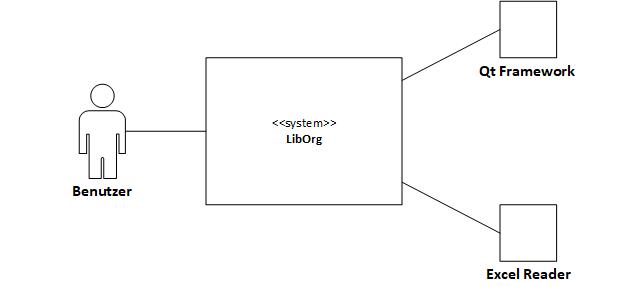
\includegraphics[width=0.50\textwidth]{figures/Fachlicher_Kontext.jpg}
	\caption{Fachlicher Kontext von LibOrg}
	\label{fig:usermanagement}
\end{figure}
\subsubsection{Benutzer}
Das Programm LibOrg dient zur Verwaltung der Bücher und der Ausleihen einer Schulbücherei. Dafür muss ein Benutzer mit dem Programm interagieren und über unterschiedliche Masken Daten mit dem Programm austauschen. Zum Beispiel können neue Bücher hinzugefügt oder ein Buch an einen Schüler ausgeliehen werden.
\subsubsection{QT Framework(Fremdsystem)}
Die GUIs über die der Benutzer mit dem Programm interagiert wurden mithilfe des Qt Frameworks erstellt. Die Verwendung des Qt Frameworks vereinfacht die Erstellung von Benutzeroberflächen.
\subsubsection{Excel Reader(Fremdsystem)}
Um die Schülerdaten aus den vorhanden Excel-Dateien (altes Excel-Format) eilesen zu können wird ein Reader benötigt. Als Excel Reader wurde FreeXL verwendet. 

\subsection{Technischer Kontext}
\begin{figure}[H]
	\centering
		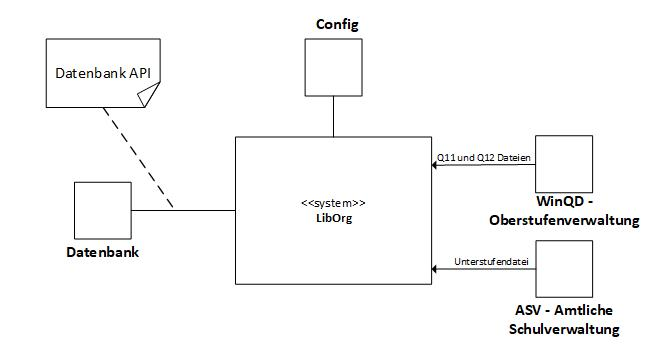
\includegraphics[width=0.50\textwidth]{figures/Technischer_Kontext.jpg}
	\caption{Technische Interaktionen von LibOrg}
	\label{fig:Technischer Kontext}
\end{figure}
\subsubsection{ASV - Amtliche Schulverwaltung}
\label{DEF:ASV}
Aus dem Schülerverwaltungsprogramm der Schule, der ASV - Amtliche Schulverwaltung, werden die Schülerdateien als Excel-Dateien exportiert. Diese Dateien enthalten die Daten der einzelnen Schüler, sowie deren Klassen. Nicht enthalten sind die Kurse von Oberstufenschülern. Es erfolgt kein direkter Zugriff von LibOrg auf ASV.

\subsubsection{WinQD - Oberstufenverwaltung}
\label{DEF:WINQD}
Für die Oberstufe werden die Daten aus dem Programm WinQD exportiert. Hierbei wird jeweils für die Q11 und die Q12 eine Datei erzeugt. Diese enthält die Kurse des aktuellen Schuljahres der Schüler. Auch hier erfolgt kein direkter Zugriff von LibOrg auf WinQD.

\subsubsection{Konfiguration}
Die grundlegenden Einstellungen des LibOrg Programms, wie die gewünschte Hintergrundfarbe, die Abkürzungen der Schulfächer, oder auch der zuletzt angemeldete Benutzer, werden in einer Konfigurationsdatei gespeichert. Diese wird immer zu Beginn des Programms gelesen und die Einstellungen in die Anwendung übernommen. Wenn die Einstellungen geändert werden, werden diese in die Konfigurationsdatei geschrieben, damit sie beim nächsten Programmstart zur Verfügung stehen.

\subsubsection{Datenbank}
Zur Speicherung aller anfallenden Daten des Programms wird eine SQLite Datenbank verwendet. Auf diese wird ausschließlich über eine eigens für die Datenbank geschriebene API zugegriffen. Die API stellt die einheitliche Speicherung, sowie den ordnungsgemäßen Zugriff auf die Datenbank sicher. 
	\newpage
	\section{Lösungsstrategie (DH)}
Um den Einstieg in die Lösung zu vereinfachen, ordnet Tabelle \ref{tab:QualitätszieleUndArchitekturansätze} den Qualitätszielen die Architekturansätze gegenüber. Abbildung \ref{fig:Loesungsansaetze_Ueberblick} verdeutlicht Aspekte der Systemarchitektur.
\begin{table}[htb]
	\centering
	\caption{Qualitätsziele und Architekturansätze}
	\label{tab:QualitätszieleUndArchitekturansätze}	
		\begin{tabular}{|l|l|}
		\hline
		Schnelle Abarbeitung der Aufträge & \textbullet{} Implementierung der Software in C++ \\
		 & \textbullet{} Vermeidung von unnötigen Arbeitswegen \\ 
		 & \textbullet{} Erläuterung der einzelnen Arbeitsschritte \\ 
		 & \textbullet{} Effiziente Implementierung der Backends \\ \hline
		Übersichtlichkeit & \textbullet{} Einhaltung von Usability-Normen \\ 
		 & \textbullet{} Einhaltung von Design-Tipps der Human Machine Interaction \\ \hline
		Verständlichkeit & \textbullet{} Einhaltung von Usability-Normen \\ 
		 & \textbullet{} Erläuterung der Dialoge \\
		 & \textbullet{} Verständliche Beschriftung der Eingabeelemente \\ \hline
		\end{tabular}
\end{table}
\begin{figure}[htb]
	\centering
		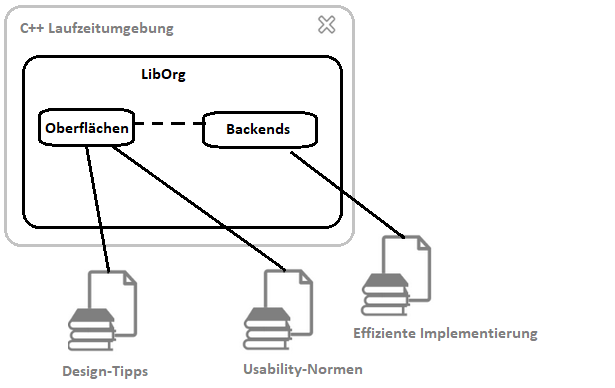
\includegraphics[width=0.60\textwidth]{figures/Loesungsansaetze_Ueberblick.png}
	\caption{Architekturaspekte Überblick}
	\label{fig:Loesungsansaetze_Ueberblick}
\end{figure}


\subsection{Aufbau von LibOrg}
LibOrg ist mittels C++ programmiert. Es ist wie folgt aufgeteilt:
\begin{itemize}
	\item db.dll: Schnittstelle zwischen der Anwendung und der Datenbank
	\item ExcelReader.dll: C++-Klasse zum Auslesen von Excel-Tabellen
	\item baseqt.dll: API, die Standardaufgaben übernimmt (z.B. Konfigurationen)
	\item Hauptanwendung
\end{itemize}
Durch die Aufteilung der Anwendung in die oben genannten Teile und die dynamische Verbindung zwischen ihnen ist es möglich, die Implementierung der entwickelten Bibliotheken (DLLs) zu erneuern, ohne dass die Hauptanwendung selber aktualisiert werden muss. Zudem wird der Wartungsaufwand der Anwendung erleichtert, da die Bibliotheken auch in anderen Projekten eingesetzt werden können (v.a. der ExcelReader und baseqt). Durch die Aufteilung der Anwendung in DLLs ist es ferner möglich, für jede DLL eigene Unit-Tests (falls gewünscht) zu entwickeln. Dies vereinfacht die Erstellung der Unit-Tests.\bigskip \\
Die Kommunikation der oben genannten Bestandteile der Software (DLLs und Hauptanwendung) erfolgt über Klassen. Bei der Implementierung der Klassen ist darauf geachtet worden, dass diese effizient und zugleich ohne lange Einarbeitungszeiten verständlich bzw. leserlich sind.\bigskip \\
Im Zentrum des Entwurfs der Strukturen liegt die Ausleihe/Rückgabe von Büchern: Für die Ausleihe wird ein Schüler-Objekt benötigt, ein Schüler kann mehrere oder keine Ausleihen haben. Außerdem ist eine Buch-Struktur notwendig, die ausgeliehen/zurückgeben wird. Die Datenstruktur für die Ausleihe enthält eine Struktur für die entsprechende Rückgabe. Das Zusammenspiel dieser Strukturen ist im Domänenmodell unter \ref{sec:domaenen} genauer verdeutlicht. Die Funktionsweise der Ausleihe/Rückgabe ist durch die Hauptanwendung definiert, wobei die Datenhaltung mit einer SQLite-Datenbank geregelt ist. Die Kommunikation findet über die Datenbank-API statt.


\subsection{Anbindungen}
LibOrg wird über eine grafische Benutzeroberfläche bzw. über grafische Benutzeroberflächen gesteuert. Die Interaktion mit dem Benutzer findet folglich über die Oberflächen statt, wobei der Benutzer durch einleitende Texte an die Verwendung der Software herangeführt wird.\bigskip \\
Durch den Einsatz von Qt arbeiten die Oberflächen mit dem Signal-Slot-Mechanismus, dieser entspricht dem Event-Ansatz. Beim Event-Ansatz wird von einem Element des GUI ein Event ausgelöst, das wiederum in einer Event-Loop abgearbeitet wird. Längere Arbeitsschritte müssen daher in eigenen Threads abgearbeitet werden, da anderenfalls die grafische Oberfläche nicht reagieren kann.\bigskip \\
An die Anwendung ist eine Datenbank (SQLite) angebunden. Die Software besitzt keine Schnittstellen nach außen, d.h. es können keine externen Funktionen in die Software eingebaut werden (die Software besitzt kein Plugin-System nach außen).
 % requires label sec:domaenen (Domänenmodell)
	\newpage
	\section{Bausteinsicht (JH)}
Dieser Abschnitt beschreibt die Zerlegung von LibOrg in Module. Die unterschiedlichen Module stellen die DLLs, sowie die Hauptanwendung dar. Im folgenden werden die Module, inklusive ihrer Schnittstellen, beschrieben.
\begin{figure}[H]
	\centering
		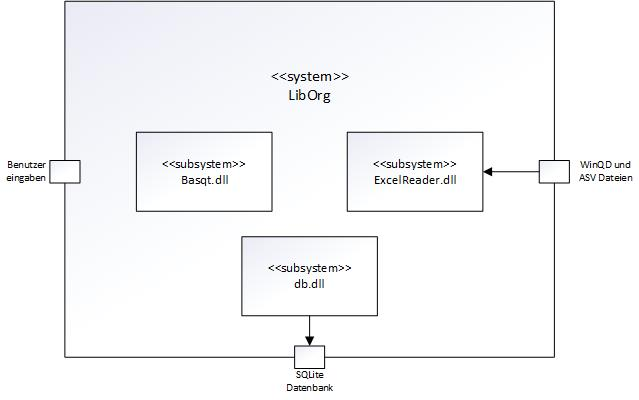
\includegraphics[width=0.60\textwidth]{figures/Bausteinschicht.jpg}
	\caption{LibOrg, Bausteinsicht}
	\label{fig:Bausteinsicht}
\end{figure}  
\begin{table}[H]
\begin{tabular}{|l|l|}
\hline
Modul           & Kurzbeschreibung                                                                                                                    \\ \hline
db.dll          & Realisiert die Kommunikation und den Datenaustausch mit der Datenbank.                                                              \\ \hline
ExcelReader.dll & Beinhaltet die Funktionalität, zum Import der Schülerdaten aus den  \\
				& ASV- und WinQD-Dateien\\ \hline
baseqt.dll      & Enthält einige grundlegende Funktionen der Anwendung, darunter den About- und  \\ 
				& den Settingsdialog und die Funktionalität der Config. \\ \hline
LibOrg          & Die eigentliche Hauptanwendung, dient zum Verwalten der Schüler und Bücherdaten.  \\  
				& Sowie die Ausleihen und Rückgaben der Bücher. \\ \hline 
\end{tabular}
\end{table}


\subsection{Db.dll}
\subsubsection{Zweck}
Dieses Modul realisiert die Kommunikation mit der Datenbank. Hierzu stellt es alle 
benötigten Funktionen bereit, um Daten in die Datenbank zu schreiben und auszulesen. 
Dafür wird eine Funktion des Moduls von der Hauptanwendung mit den erforderlichen 
Daten aufgerufen. Diese Funktion formatiert die Daten als funktionsfähiges SQL Statement
und ruft dieses auf der SQLite Datenbank auf. Dadurch wird die Integrität der Datenbank 
sichergestellt. Zusätzlich zu dieser Datenbank API, enthält die db.dll außerdem noch den 
Importdialog des ExcelReaders, die Funktionalität für das Datenbankbackup und den Logindialog.  
\subsubsection{Wichtige Funktionen}
\begin{figure}[H]
	\centering
		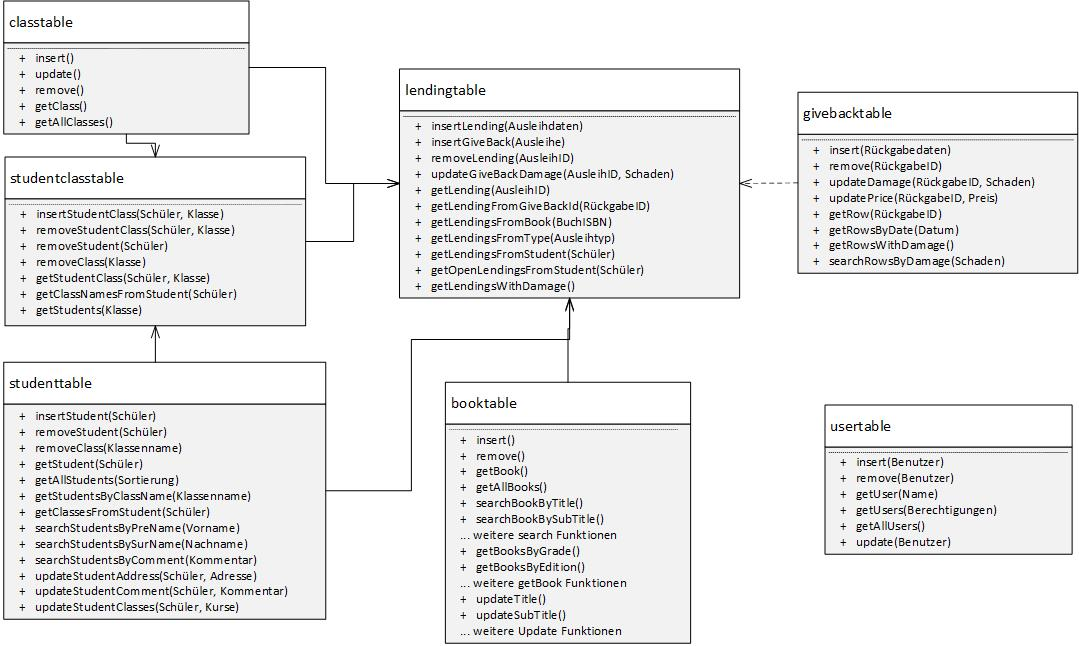
\includegraphics[width=0.95\textwidth]{figures/dbDLL.jpg}
	\caption{Überblick über die wichtigsten Funktionen der Datenbank API}
	\label{fig:dbDLL}
\end{figure}
\subsubsection{Ablageort/Datei}
Die Implementierung liegt unterhalb von Source.db.
\subsubsection{Offene Punkte}
Die Implemntierung dieses Datenbankinterfaces ist genau auf die Verwendung mit LibOrg
zugeschnitten, daher gibt es keine offenen Punkte. Allerdings muss das Interface bei 
Verwendung mit einer anderen Anwendung angepasst werden.


\subsection{ExcelReader.dll}
\subsubsection{Zweck}
Dieses Modul realisiert den Import der Schülerdaten zu Beginn des Schuljahres. Dafür 
liest es die verfügbaren Daten aus den WinQD- und ASV-Dateien aus. Bei diesen Dateien
handelt es sich um Daten in Tabellenform. Das Programm interpretiert die Daten, schreibt
die benötigten in die Datenbank und verwirft die überflüssigen. Natürlich setzt der 
ExcelReader voraus, dass die Formatierung der Dateien immer gleich vorliegt. Ebenso 
stellt er eine Fehlererkennung mit einer detailierten Ausgabe der, während des Imports
aufgetretenen, Fehler bereit.    
\subsubsection{Wichtige Funktionen}
\begin{figure}[H]
	\centering
		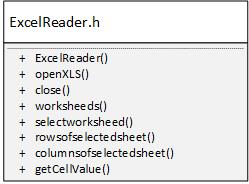
\includegraphics[width=0.30\textwidth]{figures/ExcelReader.jpg}
	\caption{Überblick über die wichtigsten Funktionen des ExcelReaders}
	\label{fig:ExcelReader}
\end{figure}
\subsubsection{Ablageort/Datei}
Die Implementierung liegt unterhalb von Source.ExcelReader.
\subsubsection{Offene Punkte}
Der ExcelReader ist vollständig Implementiert, jedoch könnte zur Erhöhung der Benutzerfreundlichkeit, noch eine direkte Fehlerbehandlung hinzugefügt werden.


\subsection{Baseqt.dll}
\subsubsection{Zweck}
Dieses Modul realisiert einige grundlegende Funktionen, welche zwar für das
Programm nötig sind, sich aber von den Grundfunktionalitäten trennen lassen. 
Daher können diese Funktionen in eine DLL ausgelagert werden. Zu diesen 
Funktionalitäten gehören:
\begin{enumerate}
\item{Überdialog}\\
	Ein Dialog, welcher Informationen über das Programm gibt, z.B. welche Version
	momentan installiert ist.
\item{Base Excpetion}\\
	Eine grunglegende Funktion um Exceptions, mit ErrorCode und Erklärung, zu verarbeiten.
\item{Konfiguration}\\
	Stellt die Funktionalität bereit, um grunglegende Einstellungen in einer Config-Datei
	zu speichern und danach zu laden.
\item{Lizenzplugin}\\
	Ein Dialog, welcher die GPL-Lizenz anzeigt, um auf die Verwendung dieser Lizenz hinzuweisen.
\item{Einstellungsdialog}\\
	Ein Dialog, um die grundlegenden Einstellung zu bearbeiten. Diese Einstellungen werden dann
	in der Konfigurationsdatei gespeichert.
\end{enumerate} 
\subsubsection{Wichtige Funktionen}
\begin{figure}[H]
	\centering
		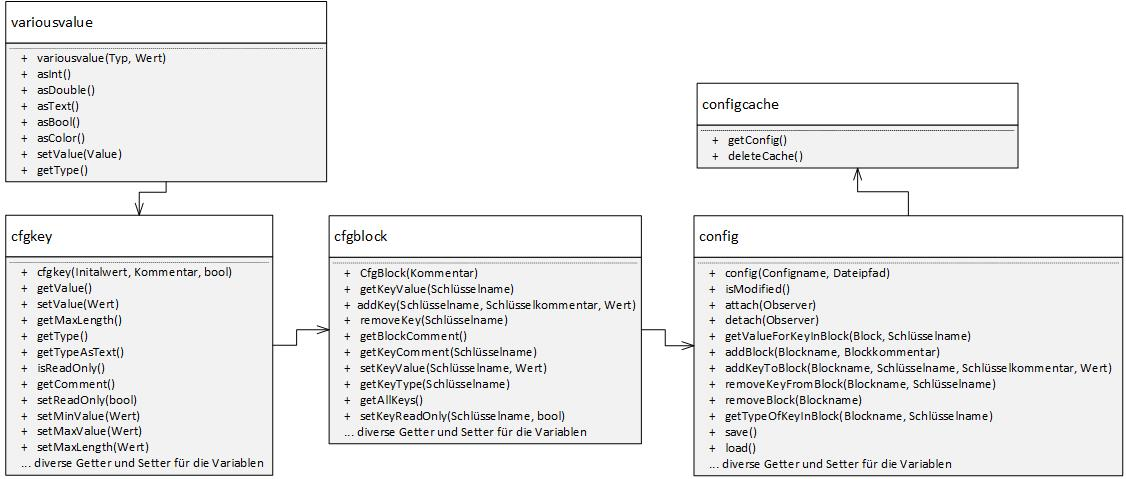
\includegraphics[width=0.95\textwidth]{figures/baseqt.jpg}
	\caption{Überblick über die wichtigsten Funktionen der Config in baseqt}
	\label{fig:baseqt}
\end{figure}
\subsubsection{Ablageort/Datei}
Die Implementierung liegt unterhalb von Source.baseqt.
\subsubsection{Offene Punkte}
Die Implementierung ist im Rahmen des Programms vollständig.


\subsection{Hauptanwendung LibOrg}
\subsubsection{Zweck}
Dieses Modul realisiert die Hauptanwendung der Software, daher stellt es alle Funktionen 
bereit, um Schüler und Bücher hinzuzufügen, zu bearbeiten oder zu löschen. Zusätzlich 
werden hier die Ausleihe- und Rückgabevorgänge abgebildet. Ebenso wird das GUI hier 
verwaltet und initalisiert. Dieses Modul enthält die Main-Funktion.
\subsubsection{Wichtige Funktionen}
\begin{figure}[H]
	\centering
		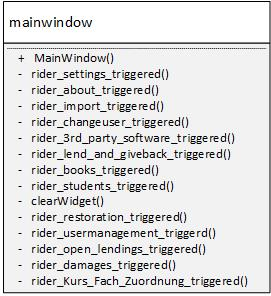
\includegraphics[width=0.20\textwidth]{figures/Mainwindow.jpg}
	\caption{Überblick über die Slots des Mainwindows }
	\label{fig:LibOrg}
\end{figure}

\subsubsection{Ablageort/Datei}
Die Implementierung liegt unterhalb von Sourc.MainProject.
\subsubsection{Offene Punkte}
Da es sich hierbei um die Hauptanwendung handelt, muss dieses Modul, für jedes neue Feature,
abgeändert werden. Für den Realesstand 1.0 ist die Implementierung vollständig.
	\newpage
	\section{Laufzeitsicht (FA)}
Nachfolgend sollen die dynamischen Aspekte des Systems dargestellt werden. Dabei wird aufgezeigt, wie die unterschiedlichen Teile der Software bei den grundlegenden Funktionen der Software zusammen spielen.

\subsection{Anlegen eines Schülers}
\begin{figure}[H]
	\centering
	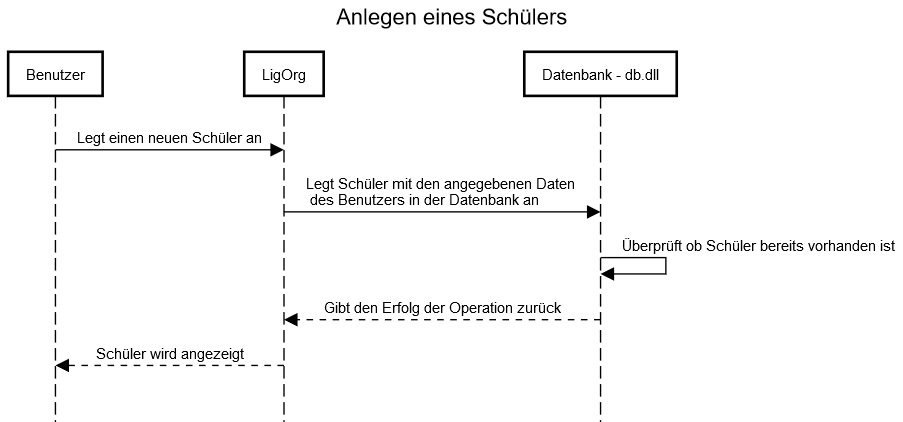
\includegraphics[width=0.80\textwidth]{figures/laufzeit/newstudent.png}
	\caption{Ablauf für das Anlegen eines Schülers}
	\label{fig:newstudent}
\end{figure}
Zunächst gibt der Benutzer die benötigten Daten in die Eingabemaske ein und bestätigt in der Benutzeroberfläche, dass er den neuen Schüler anlegen will. Daraufhin ruft die Hauptanwendung LibOrg die entsprechende Funktion der Datenbank-API auf, welche in der Datenbank den Schüler mit den vom Nutzer angegebenen Daten anlegt. Hier wird überprüft, ob der Schüler eventuell schon vorhanden ist. Nach der Ausführung der oben genannten Funktion der Datenbank-API, wird der Hauptanwendung mitgeteilt, ob der Schüler erfolgreich angelegt wurde. Wenn dies der Fall ist wird der angelegte Schüler fortan für den Benutzer angezeigt.

\subsection{Löschen eines Schülers}
\begin{figure}[H]
	\centering
	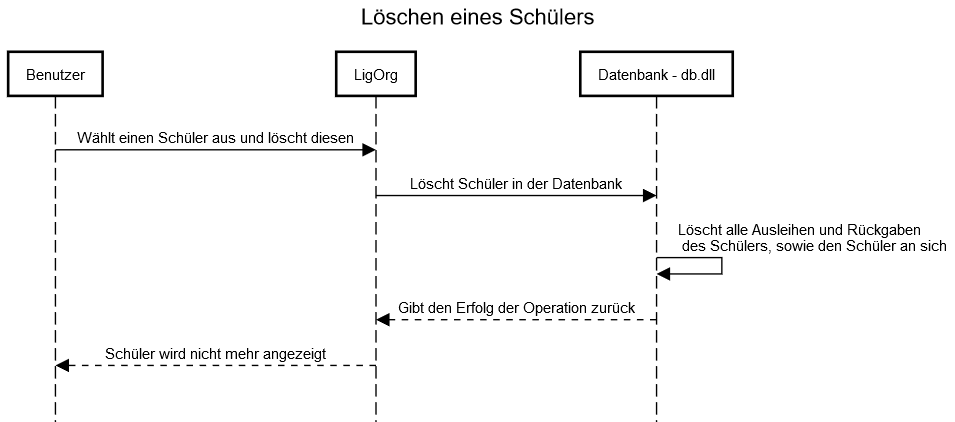
\includegraphics[width=0.80\textwidth]{figures/laufzeit/removestudent.png}
	\caption{Ablauf für das Löschen eines Schülers}
	\label{fig:removestudent}
\end{figure}
Hier wird vom Benutzer der zu löschende Schüler ausgewählt, daraufhin erscheint eine Sicherheitsabfrage, ob der Schüler wirklich gelöscht werden soll (die Sicherheitsabfrage weist auch darauf hin, ob ein Schüler noch offene Ausleihen besitzt). Wird dies bestätigt, ruft die Hauptanwendung die entsprechende Funktion der Datenbank-API auf mit den Daten des ausgewählten Schülers. Innerhalb der Datenbank werden zunächst alle Ausleihen und Rückgaben dieses Schülers gelöscht. Daraufhin wird auch noch der Schüler gelöscht. Der Hauptanwendung wird das Ergebnis der Operation mitgeteilt und der Schüler wird fortan nicht mehr angezeigt.

\subsection{Anlegen eines Buches}
\begin{figure}[H]
	\centering
	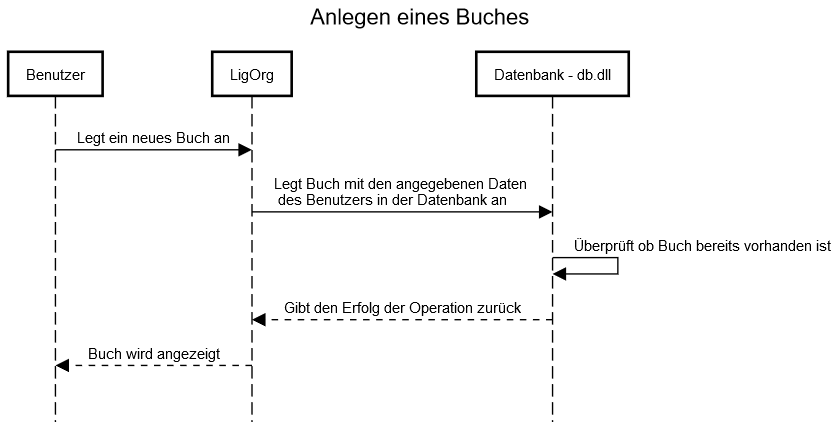
\includegraphics[width=0.80\textwidth]{figures/laufzeit/newbook.png}
	\caption{Ablauf für das Anlegen eines Buches}
	\label{fig:newbook}
\end{figure}
Anfänglich gibt der Benutzer die nötigen Daten des neuen Buches in die Eingabemaske ein und bestätigt die Erstellung des Buches. Die Hauptanwendung gibt die Daten an die entsprechende Funktion der Datenbank-API weiter, diese legt das Buch in der Datenbank an. Dabei wird überprüft, ob das Buch bereits vorhanden ist. Die Datenbank-API gibt das Ergebnis der Operation an die Hauptanwendung zurück und das neue Buch wird bei Erfolg angezeigt.

\subsection{Löschen eines Buches}
\begin{figure}[H]
	\centering
	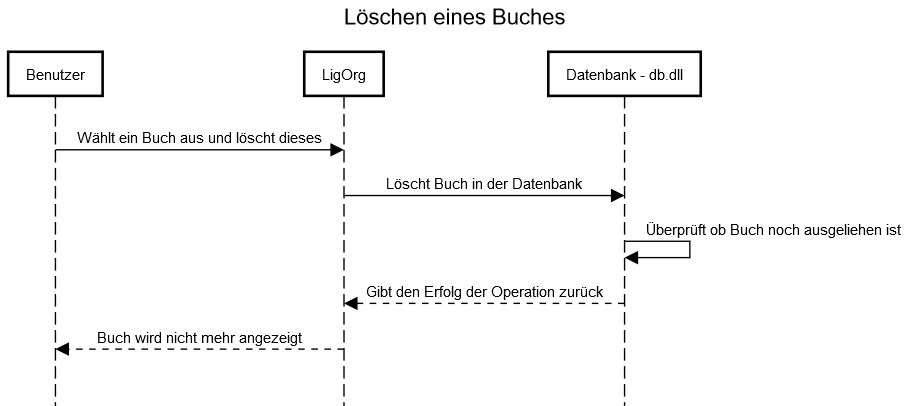
\includegraphics[width=0.80\textwidth]{figures/laufzeit/removebook.png}
	\caption{Ablauf für das Löschen eines Buches}
	\label{fig:removebook}
\end{figure}
Der Benutzer wählt das zu löschende Buch aus und bestätigt die Operation durch eine Sicherheitsabfrage. Die Hauptanwendung gibt daraufhin die Daten des ausgewählten Buches an die Datenbank-API weiter, welche überprüft, ob das ausgewählte Buch noch von Schülern ausgeliehen ist. Ist dies der Fall, kann das Buch nicht gelöscht werden. Ansonsten wird der Erfolg der Operation an die Hauptanwendung zurückgegeben und das Buch wird nun nicht mehr angezeigt.

\subsection{Ausleihen eines Buches}
\begin{figure}[H]
	\centering
	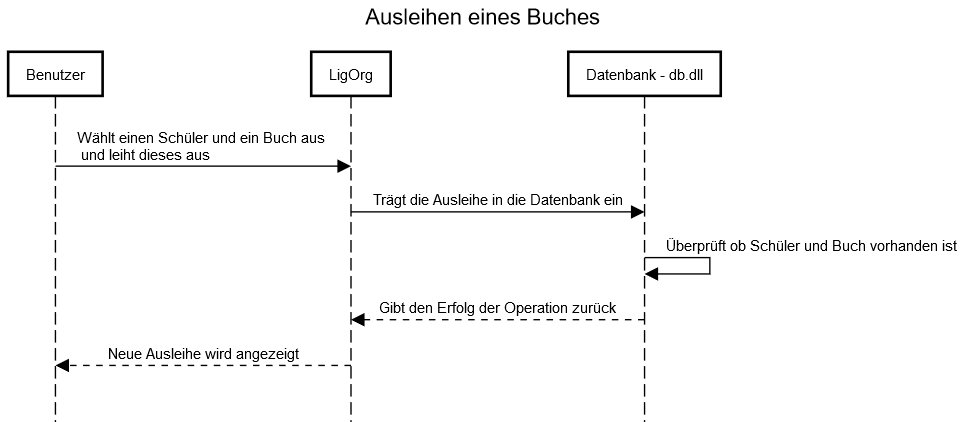
\includegraphics[width=0.80\textwidth]{figures/laufzeit/lending.png}
	\caption{Ablauf für das Ausleihen eines Buches}
	\label{fig:lending}
\end{figure}
Um eine Ausleihe anzulegen, muss der Benutzer zunächst ein Buch und einen Schüler auswählen und per Benutzeroberfläche die Ausleihe eintragen. Diese Daten werden von der Hauptanwendung an die Datenbank-API übergeben. Hier wird vorerst überprüft, ob der ausgewählte Schüler und das Buch vorhanden sind. Ist dies der Fall, wird die Ausleihe in der Datenbank eingetragen. Das Ergebnis der Operation wird an die Hauptanwendung zurückgegeben, woraufhin bei Erfolg fortan die Ausleihe in der Benutzeroberfläche angezeigt wird.

\subsection{Zurückgeben eines Buches}
\begin{figure}[H]
	\centering
	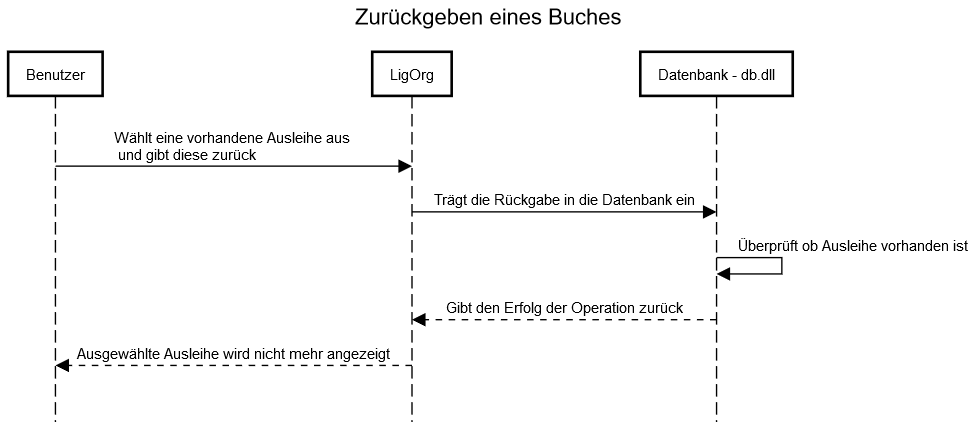
\includegraphics[width=0.80\textwidth]{figures/laufzeit/giveback.png}
	\caption{Ablauf für das Zurückgeben eines Buches}
	\label{fig:giveback}
\end{figure}
Bei dieser Operation muss der Benutzer eine bestehende Ausleihe auswählen und diese per Benutzeroberfläche zurückgeben. Die Daten der ausgewählten Ausleihe werden an die Datenbank-API übergeben. Hier wird überprüft, ob die ausgewählte Ausleihe wirklich existiert. Daraufhin wird eine Rückgabe für die entsprechende Ausleihe eingetragen. Nun wird der Erfolg der Operation zurückgegeben und die vom Benutzer ausgewählte Ausleihe wird fortan nicht weiter angezeigt. 

	\newpage
	\section{Verteilungssicht (DH)}
In der Verteilungssicht wird dargestellt, wie die Anwendung LibOrg betrieben wird. Da die Anwendung als C++-Programm umgesetzt ist, ist sie vom Betriebssystem und dessen Architektur abhängig. Damit die Architekturabhängigkeit unproblematischer wird, ist die Anwendung als 32-bit-Version compiliert worden. Damit kann die Anwendung auch auf 64-bit-Systemen ausgeführt werden. Die Betriebssystemabhängigkeit kann nur indirekt umgangen werden: Durch den Einsatz von Qt kann die Anwendung sowohl für Windows als auch für Linux und MacOS compiliert werden. Für jedes System wird daher eine eigene ausführbare Datei benötigt.\bigskip \\
Derzeit ist nur eine Version für Windows erstellt worden. Zur Installation der Anwendung auf einem Windows-PC steht ein Setup (ein Windows-Installer) zur Verfügung. Details zur Implementierung des Installers befinden sich in Anhang \ref{INSTALLER_HOWTO}.\bigskip \\
Damit die Anwendung installiert werden kann und lauffähig ist, sind folgende Voraussetzungen einzuhalten:
\begin{itemize}
	\item C++ Runtime Environment (Bestandteil von Windows)
	\item 53 MB freien Speicherplatz
	\item 1 GB Arbeitsspeicher
\end{itemize}
Bei der Installation von LibOrg werden die notwendigen dlls (dlls von Qt, baseqt.dll, ExcelReader.dll und db.dll), die Datenbank-Datei, eine Konfigurationsdatei und das Executable auf den Rechner kopiert. 

	\newpage
	\section{Konzepte (FA)}
Innerhalb dieses Kapitels werden für das Projekt allgemein gültige Strukturen und Aspekte beschrieben, welche bei der Erstellung der Software berücksichtigt werden sollen.

\subsection{Abhängigkeiten zwischen Bausteinen}
Generell sind innerhalb des Projektes folgende Bausteine zu benennen:
\begin{itemize}
	\item Hauptanwendung
	\item Datenbank-API
	\item ExcelReader
	\item baseqt
\end{itemize}
Für den Aufbau der Hauptanwendung wird die Abhängigkeit zu baseqt benötigt. Dadurch ist es möglich sämtliche notwendige Konfigurationen für die Software zu laden und zu initialisieren. Baseqt ermöglicht auch den Aufbau von Dialogen, welche grundsätzliche Informationen über die Anwendung wiedergeben. Allgemein besteht die Hauptanwendung aus einer Ansammlung an Funktionen, jede Funktion ist dabei abhängig von der Datenbank und somit von der Datenbank-API. Dies ist nötig um Daten zu lesen, abzuspeichern oder abzuändern. Die Schülerimport-Funktion benötigt außerdem eine Abhängigkeit zum Excel-Reader. Dieser wird gebraucht, um die Schülerdaten, welche in csv-Dateien abgespeichert werden in interne Datenstrukturen einzulesen und daraufhin in der Datenbank abzuspeichern.

\subsection{Domänenmodell}\label{sec:domaenen}
Innerhalb der Software sollen Schüler und deren Ausleihen und Rückgaben in einer Schulbibliothek dokumentiert werden. Um dies in einer Software abzubilden, benötigt es bestimmte Beziehungen, welche nachfolgend dargestellt werden. Die angegebenen Felder in den Abbildung sind dabei nicht vollständig und dienen hauptsächlich zur Verständnis der Beziehungen untereinander.
\begin{figure}[H]
	\centering
	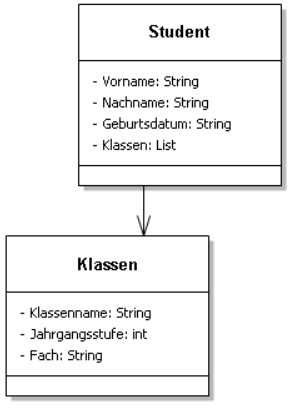
\includegraphics[width=0.30\textwidth]{figures/konzept/studclass.PNG}
	\caption{Beziehung von Schüler und Klasse}
	\label{fig:studclass}
\end{figure}
In Abbildung \ref{fig:studclass} ist die Beziehung zwischen Student und Klasse zu sehen. Jeder Student kann dabei in mehreren Klassen sein. Dies hat den Grund, dass die Oberstufen (Jahrgangsstufe 11 und 12) in verschiedenen Kursen eingetragen sind, welche innerhalb der Software auch als Klassen angelegt sind. Bis zur zehnten Jahrgangsstufe hat jeder Schüler immer nur eine Klasse. Der Schüler ist eindeutig definiert durch die Kombination des Vor- und Nachnamens, sowie des Geburtsdatums. Die Klassen sind in einer Liste hinterlegt. Eine Klasse ist durch den Klassennamen eindeutig definiert. 
\begin{figure}[H]
	\centering
	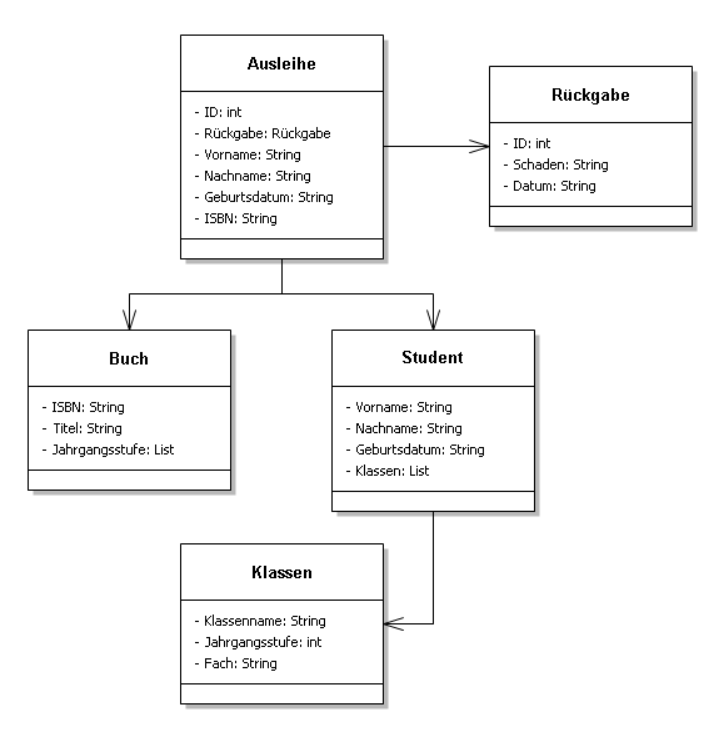
\includegraphics[width=0.55\textwidth]{figures/konzept/rueckgabe.PNG}
	\caption{Beziehungen einer Ausleihe}
	\label{fig:ausleihe}
\end{figure}
In Abbildung \ref{fig:ausleihe} sind die Beziehungen einer Ausleihe abgebildet. Eine Ausleihe benötigt dabei immer einen Studenten, welcher ausleiht, und ein Buch, welches ausgeliehen wird. Das Buch ist eindeutig definiert durch die entsprechende ISBN. Sowohl der Student, als auch das Buch werden in der Ausleihe referenziert. Eindeutig definiert ist jede Ausleihe durch einen numerischen Identifikator. Zusätzlich referenziert jede Ausleihe auf eine Rückgabe. Bei der Erstellung der Ausleihe ist diese immer leer. Erst wenn das entsprechende Buch des Studenten zurückgegeben wird, findet die Referenzierung statt. Falls das Buch Beschädigungen aufweist, werden diese ebenfalls in die Rückgabe eingetragen. Die Rückgabe ist auch durch einen numerischen Identifikator definiert.

\subsection{Benutzeroberflächen}
Sämtliche Benutzeroberflächen in LibOrg sind mittels Qt erstellt worden. Dabei beginnt das Programm derzeit immer mit einer leeren Startseite (es ist denkbar, dass in der nächsten Version der Software über die Konfiguration festgelegt wird, welches Element nach dem Starten angezeigt wird). Wählt der Benutzer in den oberen Menüleisten eine gewünschte Funktion aus, wird das entsprechende GUI angezeigt. Für die Standardfunktionen Bücher ausleihen/zurückgeben, Schüler bearbeiten und Bücher bearbeiten sind dies einfache Tabellen wie in Abbildung \ref{fig:tabelle} für das Beispiel 'Buch' zu sehen ist.
\begin{figure}[H]
	\centering
	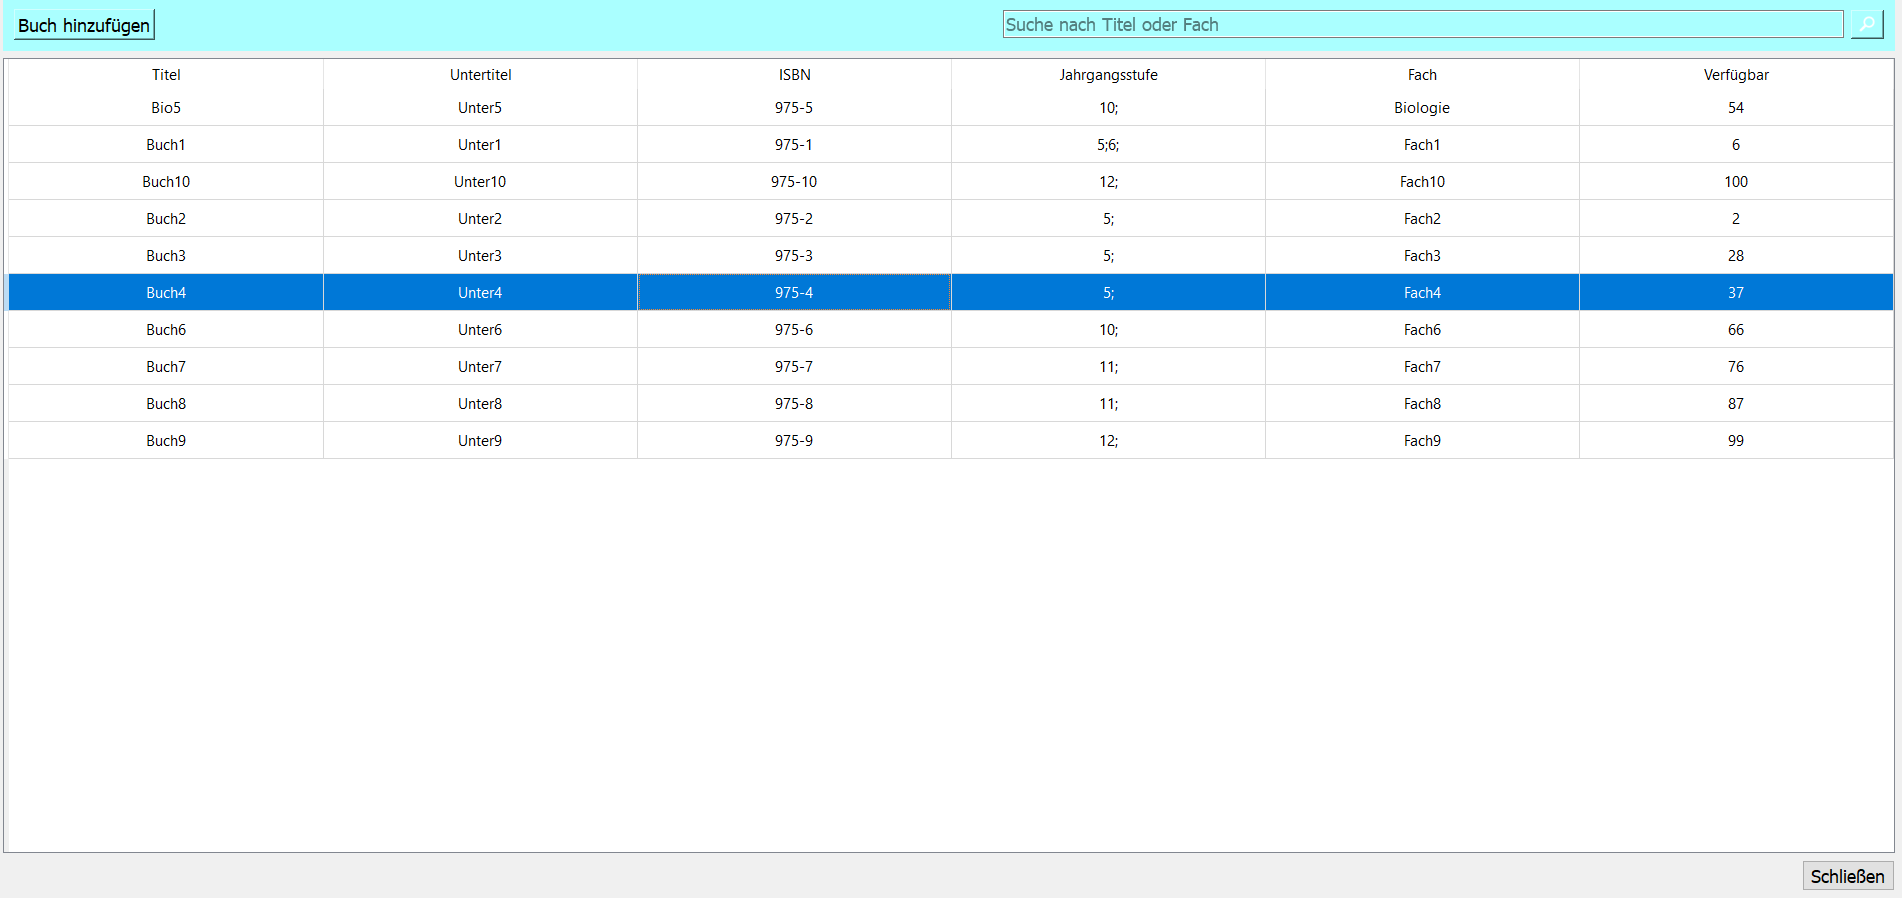
\includegraphics[width=1\textwidth]{figures/konzept/tabelle.PNG}
	\caption{Tabelle zum Anzeigen von Büchern}
	\label{fig:tabelle}
\end{figure}
Um einen Schüler oder ein Buch zu bearbeiten bzw. anzulegen, werden entsprechende Eingabemasken angezeigt, welche passende Eingabemöglichkeiten bieten (siehe Abbildung \ref{fig:maske}).
\begin{figure}[H]
	\centering
	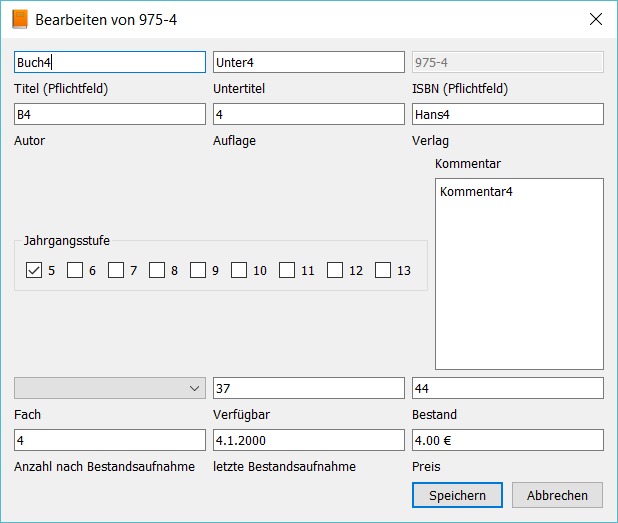
\includegraphics[width=0.60\textwidth]{figures/konzept/maske.PNG}
	\caption{Eingabemasken zum Bearbeiten eines Buches}
	\label{fig:maske}
\end{figure}
Für sonstige Aufgaben wie das Ändern der Einstellungen oder das Managen aller Benutzerkonten werden weitere passende Benutzeroberflächen angeboten.

\subsection{Plausibilisierung und Validierung}
Der Benutzer hat in LibOrg die Möglichkeit eigene Schüler und Bücher per passende Eingabemasken zu erstellen (siehe Abbildung \ref{fig:maske}). Bei der Erstellung dieser Objekte, was stattfindet sobald der Benutzer seine Angaben speichert, werden die Eingaben des Nutzers validiert. Hier wird zum Beispiel überprüft, ob ein Name oder eine ISBN (die Primary keys in der Datenbank) vorhanden sind. Für manche Einträge gibt es auch bereits fertige Eingabemasken, welche nur eine Eingabe in der vorgegebenen Form erlauben, beispielsweise das Angeben eines Datums für die letzte Bestandsaufnahme oder ein Preis für das Buch. Auch wird verboten in manchen Felder Zahlen bzw. Buchstaben anzugeben. Ein Vor- oder Nachname kann keine Zahl beinhalten und der Bestand kann nur durch Ziffern angegeben werden. Durch in grau dargestellte Platzhalter, werden dem Benutzer für jedes Feld korrekte Beispiele für die Eingabe angezeigt, wie in Abbildung \ref{fig:grey} zusehen ist.
\begin{figure}[H]
	\centering
	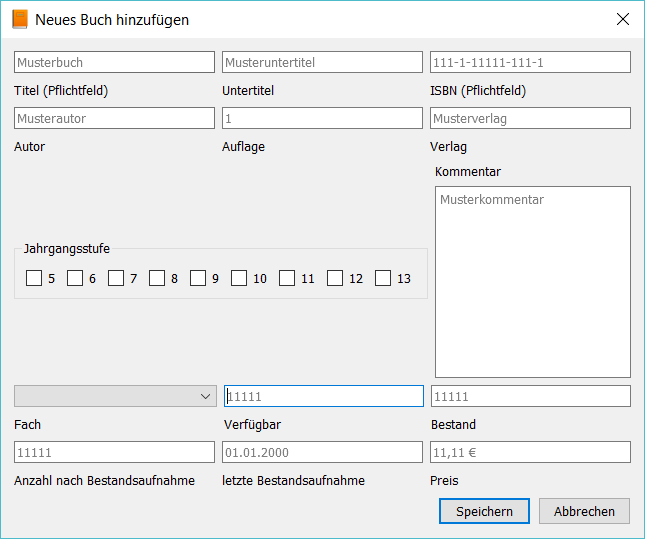
\includegraphics[width=0.60\textwidth]{figures/konzept/grey.PNG}
	\caption{Graue Platzhalter in der Eingabemaske}
	\label{fig:grey}
\end{figure}
Bei sensiblen Operation wie das Löschen eines Schülers oder eines Buches, wird der Benutzer mittels Messagebox nochmal um sein Einverständnis gefragt, damit eine versehentliche Benutzung ausgeschlossen werden kann (siehe Abbildung \ref{fig:messagebox}).
\begin{figure}[H]
	\centering
	
\includegraphics[width=0.30\textwidth]{figures/konzept/messagebox.PNG}
	\caption{Messagebox zur Bestätigung einer Operation.}
	\label{fig:messagebox}
\end{figure}

\subsection{Ausnahme- und Fehlerhandling}
Sämtliche Fehlerfälle welche durch das falsche Bedienen der Software ausgelöst werden können, werden von LibOrg abgefangen. Dabei wird dem Benutzer immer mitgeteilt, dass die geplante Aktion nicht möglich ist. Ein Beispiel hierfür wäre, wenn der Benutzer ein Buch löschen will, welches noch ausgeliehen ist. Dies würde intern zu einer Inkonsistenz der Datenbank führen, da eine Ausleihe das Buch entsprechend referenziert und somit das Buch nicht gelöscht werden darf. Dabei wird dem Benutzer durch eine MessageBox angezeigt, dass dies nicht möglich ist (siehe Abbildung \ref{fig:error}).
\begin{figure}[H]
	\centering
	
\includegraphics[width=0.40\textwidth]{figures/konzept/error.PNG}
	\caption{Messagebox zum Hinweisen des Benutzers}
	\label{fig:error}
\end{figure}
Ein Spezialfall bildet der Import von Schülern über Excel-Dateien. Da die benötigten Informationen über mehrere Excel-Dateien verteilt sind, müssen die einzelnen Schüler anhand der Namen in den einzelnen Dateien zusammengefügt werden. Hier kann es zu möglichen Fehlerfällen kommen. Zum Beispiel können die Namen der Schüler nicht genau übereinstimmen aufgrund von exotischen Namensgebungen. Auch könnte der Schüler in einer Datei existieren und in der anderen allerdings keinen Eintrag haben, dies führt ebenfalls zu einem Fehler. Nach dem Abschluss des Imports werden alle aufgetretene Fehler in einem Fenster angezeigt, wie in Abbildung \ref{fig:import} zu sehen ist. Daraufhin hat der Benutzer die Möglichkeit die Fehler über die gegebenen Standardfunktionen per Hand zu beheben.
\begin{figure}[H]
	\centering
	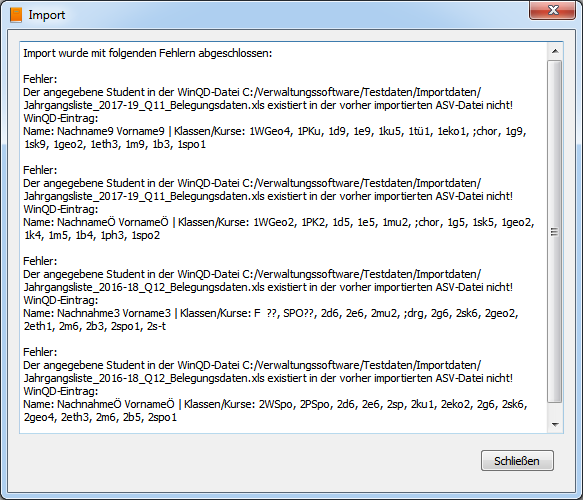
\includegraphics[width=0.60\textwidth]{figures/konzept/import.PNG}
	\caption{Fehlerausgabe nach abgeschlossenem Import.}
	\label{fig:import}
\end{figure}
Falls Daten von dem Benutzer fälschlicherweise gelöscht oder geändert werden, legt das System sicherheitshalber bei Start und beim Beenden des Programms ein Backup der aktuellen Datenbank ab. Dadurch ist es möglich jederzeit zu einem alten Stand der Datenbank zurückzukehren.

\subsection{Testbarkeit}
In LibOrg wurden sämtliche Benutzeroberflächen und die Logik dahinter 'per Hand' getestet. Hierbei wurden Excel-Listen über alle gewünschten Funktionalitäten der einzelnen Features angelegt, welche durchgegangen worden sind. \\
Per Unit-Tests wurde die komplette Datenbank-API getestet. Dies hat nicht nur den Grund, dass die komplette Anwendung auf der korrekten Funktionalität dieser API fußt, sondern auch, dass falls später die Datenbank noch erweitert wird, die Funktionalität der bisherigen API weiterhin bestätigt werden kann und dass die Änderung keine Auswirkungen auf den unveränderten Code hat (Regressionstest).

	\newpage
	\section{Entwurfsentscheidungen (DH)}
In diesem Kapitel werden grundlegende Entwurfsentscheidungen vorgestellt.

\subsection{Aufteilung des Quellcodes}
\textbf{Zur Fragestellung}\\
Die Anwendung muss einfach zu warten und zu pflegen sein. Dabei soll die Struktur der Anwendung, also die Quellcodestruktur, übersichtlich gestaltet sein. Hier stellt sich nun die Frage, wie der Quellcode am besten organisiert und aufgeteilt wird.\bigskip \\
Der Quellcode kann entweder in einem einzigen Projekt oder in Bibliotheksprojekten und einem Hauptprojekt verwaltet werden.\bigskip \\
\textbf{Relevante Einflussfaktoren}
\begin{itemize}
	\item die gewählte Struktur muss für Windows, Linux und MacOS anwendbar sein
	\item betroffenes Qualitätsziel: Wartbarkeit
\end{itemize}
\textbf{Betrachtete Alternativen}\\
Wie schon erwähnt gibt es zwei Optionen: Der gesamte Quellcode kann in einem Projekt verwaltet werden, oder der Quellcode wird in ein Hauptprojekt und Bibliotheken (dlls) aufgeteilt.\\
Befindet sich der gesamte Quellcode in einem Projekt, so sind alle Funktionen und Klassen leicht innerhalb des Projektes auffindbar. Es müssen keine weiteren Verwaltungsmaßnahmen wie bei der Aufteilung in dlls beachtet werden. Durch die Aufteilung in dlls wird die Auffindbarkeit erstmal erschwert. Dies kann verbessert werden, indem die dlls sinnvoll benannt sind und die Anwendung genug Quellcodedateien besitzt. Des Weiteren bieten dlls den Vorteil, dass Code wiederverwendbar wird und sich dadurch der Wartungsaufwand, bei der Verwendung in mehreren Projekten, deutlich reduziert.\bigskip \\
\textbf{Entscheidung}\\
Da die Anwendung entsprechend viel Code erfordert und sich Teile der Anwendung in anderen Projekten wieder verwerten lassen, ist die Entscheidung, zur Aufteilung des Quellcodes, wie folgt gefallen:
\begin{itemize}
	\item baseqt.dll: enthält Klassen für die Konfiguration, sowie für die Anzeige von Lizenzen und der Version des Programmes.
	\item ExcelReader.dll: ist ein Klassenkonstrukt zum Auslesen von Exceldateien.
	\item db.dll: beinhaltet die Datenbank-API.
	\item MainProject: Hauptprojekt, dass die dlls einbindet und spezifische Funktionen implementiert.
\end{itemize}
Wie dlls in Qt erzeugt werden, ist im Anhang \ref{DLLs_HOWTO} erläutert.
	\newpage
	\section{Qualitätsszenarien (DH)}
In diesem Kapitel werden Szenarien vorgestellt, mit denen die Qualitätsziele beispielhaft verdeutlicht werden. 

\subsection{Qualitätsbaum}
Abbildung \ref{fig:Qualitaetsbaum} liefert einen Überblick über die Qualitätsmerkmale und welche Szenarien ihnen zugeordnet sind.
\begin{figure}[htbp]
	\centering
		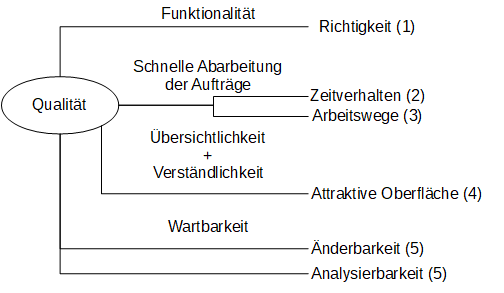
\includegraphics[width=0.50\textwidth]{figures/Qualitaetsbaum.PNG}
	\caption{Qualitätsbaum}
	\label{fig:Qualitaetsbaum}
\end{figure}

\subsection{Bewertungsszenarien}
Die Qualitätsszenarien sind:
\begin{enumerate}
	\item Die Eingabemasken filtern falsche oder fehlende Eingaben heraus und zeigen Warnungen an, so dass der Anwender die Eingaben korrigieren kann, bevor die Anwendung die Eingaben verarbeitet.
	\item Die Listen sollen innerhalb von Millisekunden angezeigt werden. Die Buchung eines Buches für alle Schüler einer Klasse soll innerhalb von 2 Sekunden erfolgt sein.
	\item Zusammengehörende Funktionen sollen über eine gemeinsame Oberfläche ausgeführt werden können. Hiermit sollen unnötige Mausklicks vermieden werden.
	\item Die Oberflächen sind ansprechend, Aufgaben werden erläutert und die Darstellung ist benutzerfreundlich (siehe Anhang \ref{USABILITY_ASPEKTE}).
	\item Der Sourcecode der Anwendung ist dokumentiert und unter Verwendung von Coding Conventions implementiert (siehe Kapitel \ref{KONVENTIONEN}). Des Weiteren ist der Code so organisiert, dass Änderungen möglichst einfach durchgeführt werden können.
\end{enumerate}
	\newpage
	\input{Risiken}
	\newpage
	\section{Unterstützungs-App (JH)}
Die Unterstützungs-App soll die Hauptanwendung um die Möglichkeit erweitern, Ausleihen und Rückgaben durch Unterstützer direkt in den Klassen durchzuführen. Zu diesem Zweck wurde eine App entwickelt, welche die genannten Funktionen bietet und (derzeit) auf einem Android-Smartphone installiert werden kann.
\subsection{Datenübertragung per Ad-Hoc Verbindung}
Um Zugriff auf die Daten der LibOrg-Anwendung zu bekommen, war ursprünglich ein Ad-Hoc-Netzwerkverbindung zwischen dem Rechner, auf dem die Hauptanwendung läuft, und der App auf einem Android-Smartphone geplant. Leider unterstützt Android Ad-Hoc-Netzwerke jedoch unerwarteterweise nicht. Aus diesem Grund musste auf die Hotspot-Technologie zurückgegriffen werden. Hierbei muss zuerst der Hotspot auf dem Android Gerät aktiviert werden und dann der Rechner, auf dem die Hauptanwendung läuft, auf diesen verbunden werden. Dies ist für den Kunden zu aufwendig, deshalb kann alternativ das Smartphone und der Laptop mit dem gleichen Access Point verbunden werden. Daraufhin muss im Hauptprogramm die Unterstützungsfunktion gestartet werden und die dort angezeigte IP-Adresse und der Port in der App eingetragen werden. Anschließend kann man Verbinden und dann von der Hauptanwendung die Datenbank an das Smartphone übertragen. Danach kann die Klassenauswahl erfolgen.
\begin{figure}[H]
	\centering
		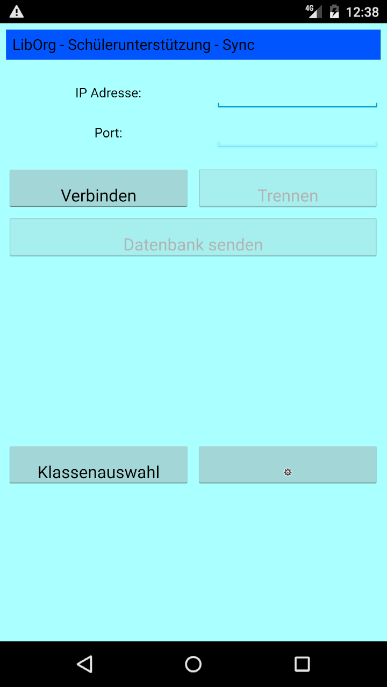
\includegraphics[width=0.30\textwidth]{figures/SupportApp/Verbindung.png}
	\caption{Verbindungsansicht der Support-App}
	\label{fig:Verbindungsansicht App}
\end{figure}

\subsection{Klassen und Schülerauswahl}
Die folgenden Dialoge bieten die Möglichkeit zuerst eine Klasse und dann einen Schüler auszuwählen. Allerdings können die Bücher auch klassenweise ausgeliehen und zurückgegeben werden.
\begin{figure}[H]
	\centering
		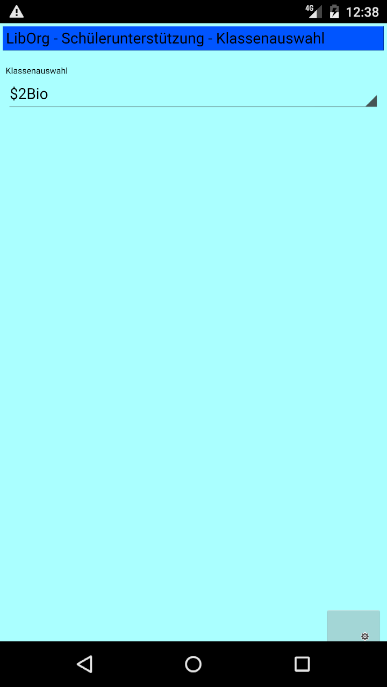
\includegraphics[width=0.30\textwidth]{figures/SupportApp/Klassenauswahl.png}
	\caption{Klassenauswahl der Support-App}
	\label{fig:Klassenauswahl App}
\end{figure}

\begin{figure}[H]
	\centering
		\includegraphics[width=0.30\textwidth]{figures/SupportApp/Schülerauswahl.png}
	\caption{Schülerauswahl der Support-App}
	\label{fig:Schülerauswahl App}
\end{figure}

\subsection{Ausleihe und Rückgabe von Büchern}
Zuletzt kommt man zur eigentlichen Funktion der App, das Ausleihen und Zurückgeben. Je nach Auswahl entweder pro Schüler oder klassenweise. Wichtig ist hierbei, dass bei der klassenweisen Rückgabe von Büchern sicher gestellt werden muss, dass kein Buch Beschädigungen aufweist, da die Überprüfung auf Schäden nur bei der Einzelrückgabe erfolgt.
\begin{figure}[H]
	\centering
		\includegraphics[width=0.30\textwidth]{figures/SupportApp/Schülerausleihe.png}
	\caption{Schülerausleihe der Support-App}
	\label{fig:Schülerausleihe App}
\end{figure}

\begin{figure}[H]
	\centering
		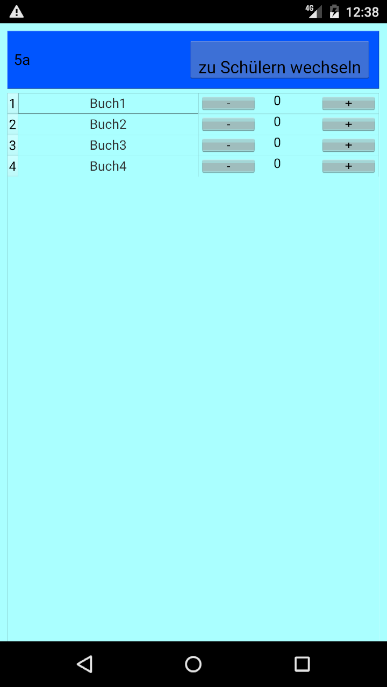
\includegraphics[width=0.30\textwidth]{figures/SupportApp/Klassenausleihe.png}
	\caption{Klassenausleihe der Support-App}
	\label{fig:Klassenausleihe App}
\end{figure}

Die App stellt eine erste Version mit den wichtigsten Funktionen dar und kann in Zukunft noch um einige Funktionalitäten erweitert werden. So kann zum Beispiel eine Abfrage der Beschädigungen in der klassenweisen Rückgabe erfolgen oder eine Ferienausleihe einzelner Bücher erfolgen. Ebenfalls kann noch vieles an der Usability und am Overlay angepasst werden. Des Weiteren könnte man mehrere Android- Geräte mit unterschiedlichen Datenbeständen losschicken und diese zum Schluss in der Hauptanwendung wieder zusammenführen. Dafür wären allerdings Änderungen in der Hauptanwendung und ein ausgeklügeltes Übertragungsprotokoll notwendig.
	\newpage
	\section{Glossar (DH)}
In diesem Abschnitt werden Begriffe, die spezifisch für LibOrg sind, erläutert.
\begin{itemize}
	\item Student(in): Schüler, beziehungsweise Schülerinnen an der Schule des Kunden.
	\item Ausleihe: Beschreibt den Vorgang, bei dem einem Student/einer Studentin ein bestimmtes Buch, für einen bestimmten Zeitraum, zur Verfügung gestellt wird. In der Datenbank der Anwendung wird ein Buchungseintrag vorgenommen.
	\item Rückgabe: Bei diesem Vorgang gibt ein Student/eine Studentin ein Buch zurück. In der Datenbank wird, an den Buchungseintrag der Ausleihe, ein Eintrag für die Rückgabe angehängt.
	\item MessageBox: Dialog, der eine Nachricht für den Anwender darstellt.
\end{itemize}
	\newpage
	
	%\section{Grundlagen des Projekts}



 


  %\newpage	
	%\section{Sofwarearchitektur}
Im folgenden werden die einzelnen Bestandteile der Sofware beschrieben. Die Abbildung veranschaulicht die Zusammenhänge. 
\begin{figure}[htb]
	\centering
		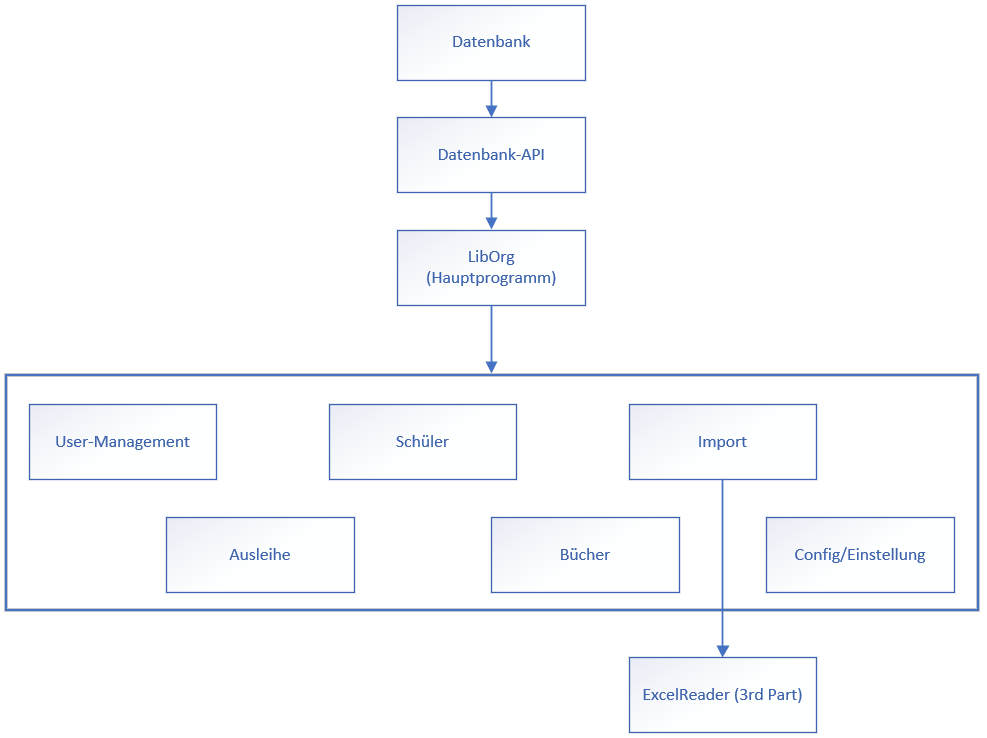
\includegraphics[width=0.90\textwidth]{figures/architecture.png}
	\caption{Die Architektur der Software}
	\label{fig:Architektur}
\end{figure}

\subsection{Datenbank}
Alle anfallenden Daten werden in einer SQLite Datenbank gespeichert. Hierfür wurden die folgenden Tabellen angelegt:
\begin{itemize}
\item BookTable \newline
bildet die im Programm verfügbaren Bücher ab \newline
primary Key: isbn -> ISBN Nummer des Buches \newline
weitere Werte: title -> Buchtitel, subtitle -> Untertitel, publisher -> Verlag, author -> Autor, subject -> Fach, grade -> Klassenstufe, edition -> Auflage, price -> Preis, stock -> auf Lager, available -> verfügbar, comment -> Kommentar, stocktakingCount -> Inventuranzahl, stocktakingDate -> Inventurdatum
\item ClassTable \newline
Klassen, sowie Fächer
\item LendingTable \newline 
Ausleihen 
\item ReturnTable \newline
Rückgaben
\item StudentClassTable \newline 
bildet den Zusammenhang zwsichen Schülern und Klassen ab 
\item StudentTable  \newline
Schüler 
\item UserTable  \newline
Benutzer 
\end{itemize} 
 

\subsection{Datenbank\-API}
Die Datenbank-API dient der Interaktion des C++ Hauptprogramms mit der SQLite Datenbank. Sie stellt alle benötigte Funktionen bereit, welche vom Hauptprogramm benötigt werden. Der Zugriff auf die Datenbank erfolgt ausschließlich über die Datenbank\-API.


\subsection{Hauptanwendung - LibOrg}
Die Grundanwendung(Liborg) stellt das Hauptfenster, das Programmmenü, die  Hilfe, sowie die obere Menüleiste bereit. Über das Programmmenü, kann man die Einstellunge, den Import, die Benutzerverwaltung, den Benutzerwechsel sowie die Backup-Wiederherstellung erreichen. Alle weiteren Funktionen werden über die Reiter der Grundanwendung aufgerufen. 
\begin{figure}[H]
	\centering
		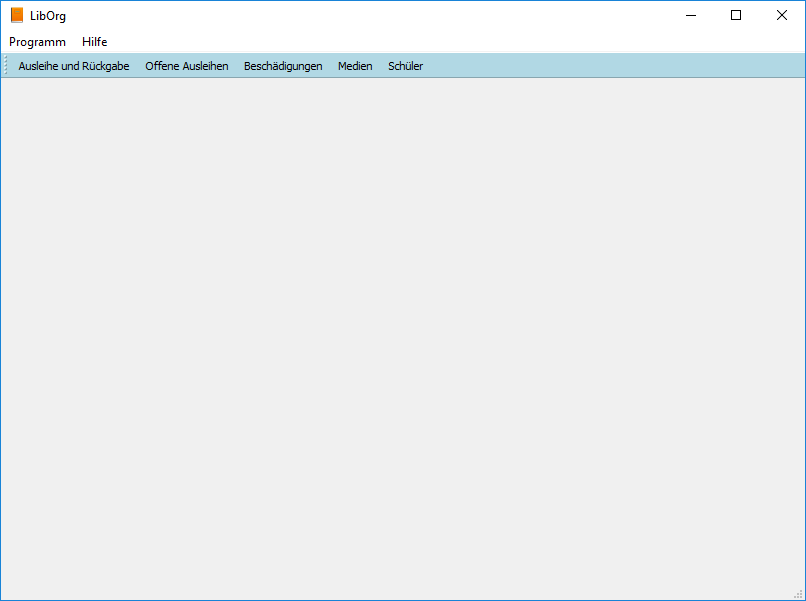
\includegraphics[width=0.70\textwidth]{figures/Liborg.png}
	\caption{LibOrg - die Grundanwendung}
	\label{fig:Mainwindow}
\end{figure}


\subsubsection{Benutzerverwaltung}
Die Benuterverwaltung erreicht man über das das den Menüpunkt "Programm" -> Benutzerverwaltung. Dort werden die Benutzer mit ihren Passwörtern und ihren Berechtigungen verwaltet. Sowie neue Benutzer angelegt und alte gelöscht.
\begin{figure}[H]
	\centering
		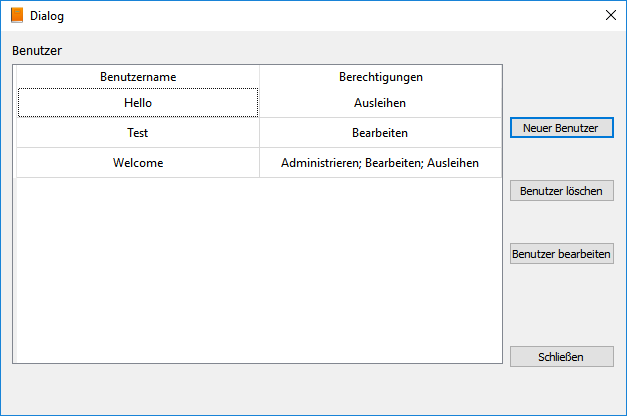
\includegraphics[width=0.70\textwidth]{figures/usermanagement.png}
	\caption{Die Benutzerverwaltung}
	\label{fig:usermanagement}
\end{figure}


\subsubsection{Ausleihe}
Die Ausleihen werden über den Reiter "Ausleihe und Rückgabe" in der Grundanwendung aufgerufen. Hier werden alle ausgeliehene Bücher mit zugehörigem Schüler gespeichert und verwaltet.
\begin{figure}[H]
	\centering
		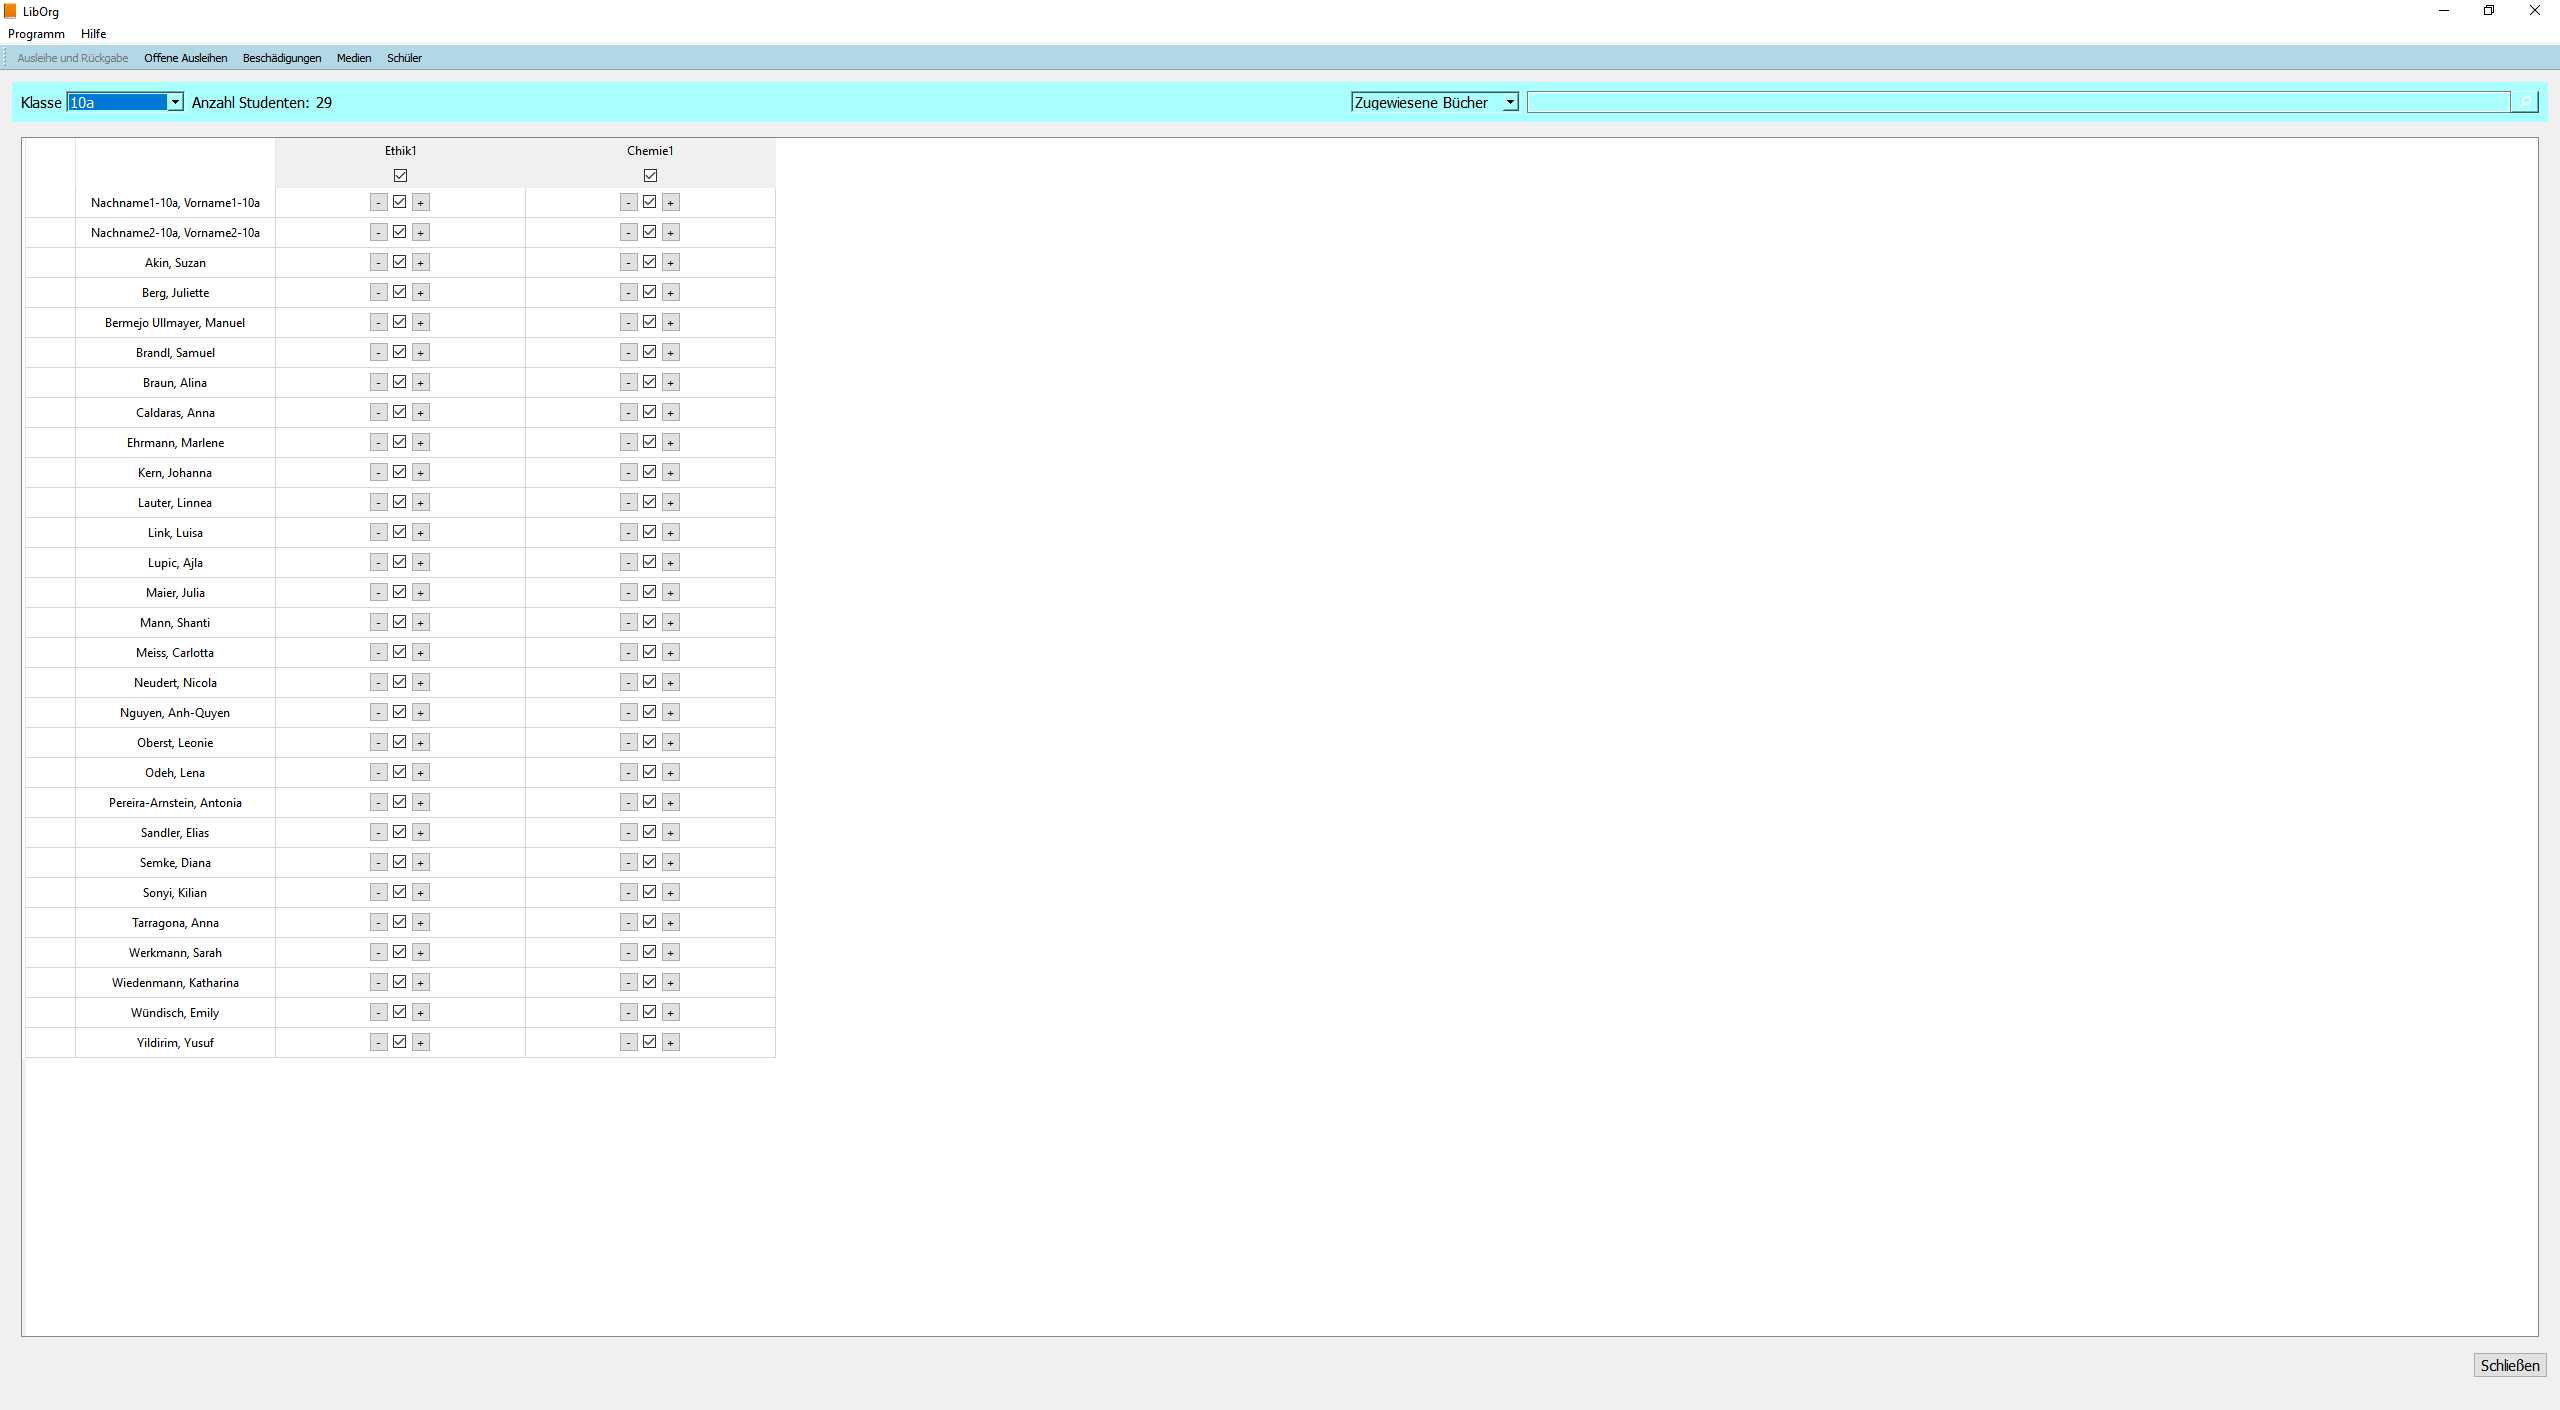
\includegraphics[width=0.70\textwidth]{figures/lendings.png}
	\caption{Ausleihe}
	\label{fig:lendings}
\end{figure}

\subsubsection{Schüler}
Hier werden Schüler angelegt und verwaltet.


\subsubsection{Bücher}
Hier werden Bücher angelegt und verwaltet.


\subsubsection{Import}
Der Import regelt die Verarbeitung der Schülerdateien, welche aus der Anwendung ASV (Amtliche Schulverwaltung), am Anfang des Schuljahres generiert werden.


\subsubsection{Config\/Einstellungen}
Die Config und die Einstellungen regeln alle Einstellung, welche auch noch nach Beenden des Programms gespeichert werden sollen und nicht in der Datenbank liegen. Das wichtigste hierbei sind die Abkürzungen der Fächer und der Back-Up Plan.



\section{Anwendung der Software}
Dieses Kapitel beschreibt die Anwendung im Produktivbetrieb. Also die Vorgänge, welche der Anwender durchführen kann.

\subsection{Anmelden/User anlegen}
Beim ersten Start der Anwendung meldet sich der Benutzer mit dem Standardbenutzer an und erstellt sich im Benutzerverwaltungs Dialog einen neuen Benuter. Hierbei  Auf diesen Benutzer wechselt er daraufhin und löscht den Standardbenutzer. 
\begin{itemize}
\item Benutzeranmeldung : mainwindow.cpp in window\_loaded\(\)
\item Öffnen der Benutzerverwaltung : mainwindow.cpp in rider\_user\_management\_triggerd\(\)
\item Neuen Benutzer anlegen : usermanagementdialog.cpp in addNewUser\(\) -> adduserdialog.cpp in apply\(\),sowie getReturnUser\(\) 
\item Benuzer wechseln : mainwindow.cpp in rider\_changeuser\_triggered\(\) -> mainwindow.cpp in window\_loaded\(\)
\item Benutzer löschen : usermanagementdialog.cpp in deleteUser\(\) 
\end{itemize}

\subsection{Einstellungen vornehmen}
Einstellungsdialog öffnen und die Einstellungen verändern. Danach werden die Einstellungen übernommen

\subsection{Import}
Importdialog öffnen und auswählen der Dateien. Starten des Imports, danach auswerten der eventuell auftretenden Fehler.

\subsection{Schüler anlegen/bearbeiten}
Auswählen des Reiters Schüler, daraufhin bearbeiten eines vorhanden bzw. anlegen eines neuen Schülers. Filterung über das Suchfeld in der linken oberen Ecke möglich.

\subsection{Bücher anlegen/bearbeiten}
Auswählen des Reiters Medien, dort bearbeiten eines vorhanden bzw. anlegen eines neuen Buches. Filterung über das Suchfeld in der linken oberen Ecke möglich.

\subsection{Ausleihe}
Auswählen des Reiters Ausleihe und Rückgabe, dort wird dann eine Klasse ausgewählt. Zusätzlich kann noch mithilfe der Suche  gefiltert werden. Danach erfolgt die Ausleihe eines Buches an einen Schüler über die CheckBox in der Zeile des Schülers, oder über die CheckBox im Kopf der Tabelle, für alle angezeigten Schüler.

\subsection{Rückgabe}
\subsubsection{Rückgabe über Ausleihe und Rückgabe}
Auswählen des Reiters Ausleihe und Rückgabe, daraufhin auswählen einer Klasse, optional filtern über das obige Suchfeld und und ebenfalss optional umschalten zwischen zugewiesenen und allen Büchern. Einzelrückgabe über die Checkbox bzw. den Plus- und Minusbutton in der Zeile des Schülers und Klassenrückgaben über die Checkbox im Kopf der Tabelle. Daraufhin bestätigen des Dialogs und bei Einzelrückgabe eintragen eventueller Beschädigungen.

\subsubsection{Rückgabe über Offene Ausleihen}
Auswählen des Reiters Ausleihen, daraufhin rechtsklick oder doppelklick auf die gewünschte Ausleihe. Im folgenden Dialog ist eine umschalten zwischen zugewiesenen und allen Büchern möglich. Daraufhin Rückgabe über die Checkbox oder über den Minus Button. Eintragen eventueller Beschädigungen und bestätigen des Dialogs.

\subsection{Ferienausleihe/Beschädigungen (Sonderfälle)}

\subsubsection{Ferienausleihe}

\subsubsection{Beschädigungen}

\subsubsection{automatisches Backup}

	%\newpage
	%\section{Fazit}
Während der Entwicklung der Import-Funktion, also dem Auslesen der Excel-Dateien hat sich herausgestellt, dass die Library FreeXL nicht verlässlich arbeitet und daher langfristig ausgetauscht werden muss. Zur Umsetzung der Tabellen ist das Model-View-Konzept von Qt verwendet worden. Dabei ist aufgefallen, dass einige Standardfeatures der View nicht vorhanden sind. So kann beispielsweise eine Spalte nicht vergrößert werden, obwohl sich lustigerweise der Mauscursor in die richtige Gestalt zur Änderung der Spaltengröße ändert. Die itembasierten Versionen der Views besitzen diese Funktionalität. Darüber hinaus musste festgestellt werden, dass die Qt-Bibliothek nicht die gewünschte Verlässlichkeit besitzt. Oftmals fehlten Funktionen, die ein Framework zur verlässlichen Verwendung bieten sollte und eigentlich als selbstverständlich angesehen worden sind. Hierzu zählt beispielsweise die fehlende Unterstützung für verschlüsselte und Passwort geschützte Datenbanken.\bigskip \\
Während des Projektes konnten leider nicht alle Features der Software implementiert werden. Wie von Anfang an vermutet, fehlte eine vierte Person. Die Software befindet sich dennoch in einem verkäuflichen Zustand. In naher Zukunft muss diese verbessert und optisch ansprechender gemacht werden.	
	%\newpage
	\section*{Literatur}
	\addcontentsline{toc}{section}{Literatur}
	\printbibliography[heading=none]
	\newpage
	
	\section*{Anhang}
	\addcontentsline{toc}{section}{Anhang}
		\renewcommand{\thesection}{\Alph{section}}
		\renewcommand{\thesubsection}{\Alph{subsection}}
		\subsection{Verwendete Tools (DH)}
Die nachfolgenden Abschnitte erläutern die eingesetzten Werkzeuge, die für das Projekt benötigt werden.

\subsubsection{Tools zur Erstellung von Videos (DH)}
Um dem Kunden den aktuellen Stand der Entwicklung zu präsentieren, werden Videos von den Teilfunktionen der Software angefertigt. Anhand dieser Videos kann der Kunde Feedback zur Software geben, ohne jedes mal eine neue Version der Software installieren zu müssen. Darüber hinaus dienen die Videos später auch dazu, die Software in Internet anzupreisen beziehungsweise Kunden einen Einblick in die Software zu gewähren. Außerdem werden die Videos der Software als Hilfe hinzugefügt.\\
Zur Erstellung von Videos werden zwei Werkzeuge benötigt: Das Open Broadcaster Studio und OpenShot. Diese beiden Tools können auf den Betriebssystemen Windows, MacOS und Linux verwendet werden und besitzen eine GPL-Lizenz. Die erstellten Videos dürfen folglich kommerziell benutzt werden.\bigskip \\
\textbf{Open Broadcaster Studio (DH)}\\
Mit dem Open Broadcaster Studio\footnote{https://obsproject.com/download} werden die Videos samt Ton aufgenommen. Die Anwendung ist in Abbildung \ref{fig:OBS} dargestellt.
\begin{figure}[htb]
	\centering
		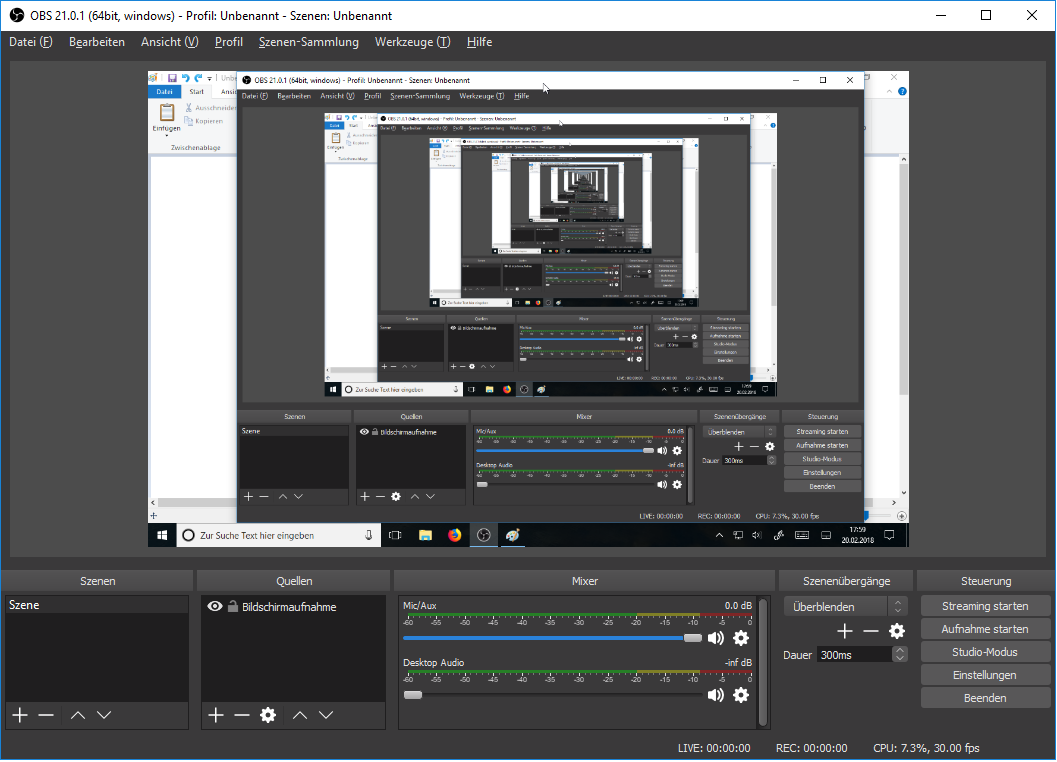
\includegraphics[width=0.70\textwidth]{figures/OBS.png}
	\caption{Open Broadcast Studio}
	\label{fig:OBS}
\end{figure}
Der Vorteil dieser Software ist, dass sie, anders als beispielsweise der VLC Media Player, die Video- und Audiosignale gleichzeitig aufnehmen kann \cite[vgl.][]{OBS}.\\
Nach der Installation führt die Anwendung eine automatische Konfiguration durch, dabei sollte die Konfiguration für die Aufnahme selektiert werden. Nach dieser Konfiguration kann überprüft werden, ob das Mikrofon gefunden wurde, indem die Signalstärke des Audiogeräts betrachtet wird. Sollte sich diese nicht beim Sprechen bewegen, so kann die Wahl des Audiogerätes über die Einstellungen vorgenommen werden. Per default wird kein Videosignal aufgenommen. Um eine Videoquelle hinzuzufügen, wird in der Quelle die Bildschirmaufnahme (mit +) ausgewählt. Um nicht ständig das erzeugte Video in ein mp4-Format zu konvertieren, ist es ratsam, unter Einstellungen - Ausgabe das Aufnahmeformat auf mp4 zu stellen. Das mp4-Format wird zwingend für Websiten benötigt, deshalb müssen Videos immer das mp4-Format haben! Eine Aufnahme wird mittels Aufnahme starten begonnen und mit Aufnahme beenden gestoppt. Die Aufnahmen befinden sich anschließend in der Regel unter "`Dieser PC"' - Videos. Dies kann über Datei - Zeige Aufnahmen herausgefunden werden \cite[vgl.][]{OBS}. \bigskip \\
\textbf{OpenShot (DH)}\\
Das Open Broadcast Studio hat einen Nachteil: Mit ihm können die aufgenommenen Videos nicht geschnitten werden. Das Programm OpenShot\footnote{https://www.openshot.org/download/} kann Videos im mp4-Format schneiden. Leider hat dieses Programm jedoch den Nachteil, dass es gerne einfriert oder abstürzt. Für die im Projekt notwendigen Schnitte kann dies jedoch akzeptiert werden. Die Anwendung ist in Abbildung \ref{fig:OpenShot} dargestellt.
\begin{figure}[htb]
	\centering
		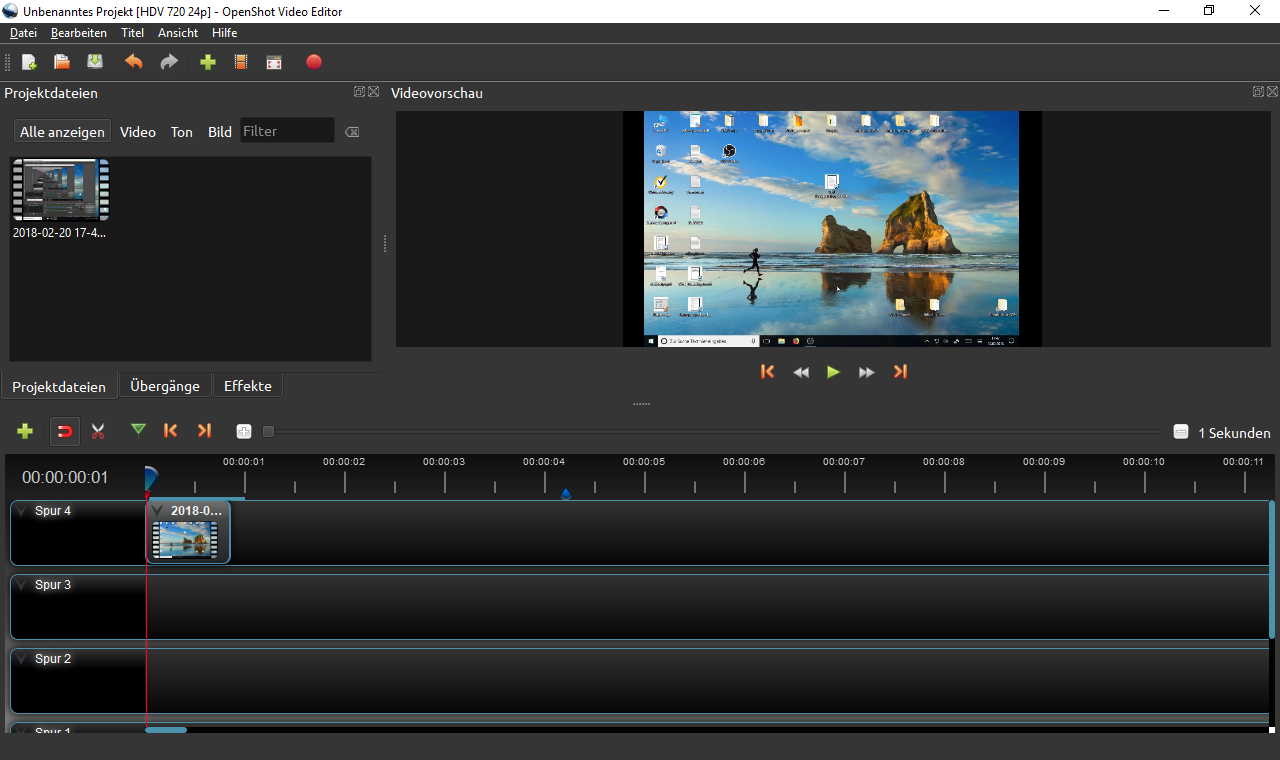
\includegraphics[width=0.70\textwidth]{figures/OpenShot.png}
	\caption{OpenShot}
	\label{fig:OpenShot}
\end{figure}
Um ein Video zu schneiden, wird im Feld Projektdateien per Rechtsklick Dateien importieren ausgewählt und die Datei selektiert, die geschnitten werden soll. Anschließend wird das importierte Video in eine Spur gezogen. Dabei sollte darauf geachtet werden, dass die Datei zum Zeitpunkt Null in der Spur liegt. Mit der roten Zeitachse wird die Stelle im Video gesucht, an der geschnitten werden soll. Ist die Stelle gefunden, wird das Schneidewerkzeug (Schere) selektiert und auf die markierte Stelle angewendet (Achtung: Dies kann etwas dauern!). Das Video wird an der entsprechenden Stelle aufgeteilt. Das Schneidewerkzeug muss nun deselektiert werden, um den Teil des Videos löschen zu können. Zum Löschen wird auf den gewünschten Teil mit Rechtsklick Video löschen ausgewählt (den Rest wieder an den Null-Punkt ziehen). Aus den Videos sollten alle Teile herausgeschnitten werden, die nicht unbedingt darin enthalten sein sollten. Dies ist zum Beispiel der Anfang und das Ende des Videos, in dem die Aufnahmefunktion gestartet beziehungsweise gestoppt wird. Zum Speichern des geschnitten Videos wird Datei - Video exportieren ausgewählt. Wichtig beim Speichern: Das Format muss erneut mp4 sein!

\subsubsection{TaskBoard (DH)}
Die einzelnen Aufgaben werden in einem TaskBoard, siehe Abbildung \ref{fig:TaskBoard}, festgehalten und können agil bearbeitet werden. Jeder Teilnehmer des Projektes erhält einen eigenen Account auf dem TaskBoard. Es kann unter https://gitlab-testbot.informatik.hs-augsburg.de/taskboard erreicht werden.
\begin{figure}[htb]
	\centering
		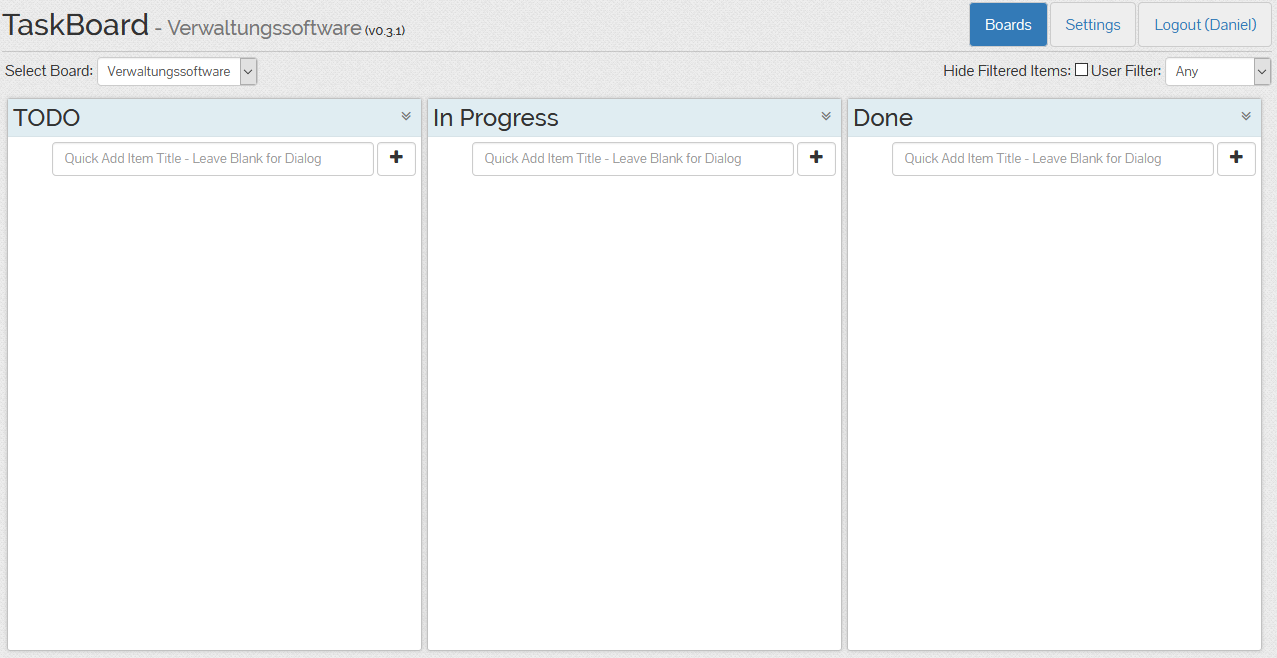
\includegraphics[width=0.70\textwidth]{figures/TaskBoard.PNG}
	\caption{TaskBoard}
	\label{fig:TaskBoard}
\end{figure}
Jedes Board des TaskBoards besteht aus drei Tabellen: 
\begin{itemize}
	\item TODO: Enthält Aufgaben, die noch zu erledigen sind
	\item In Progress: Aufgaben, die von einer Person derzeit bearbeitet werden
	\item Done: Erledigte Aufgaben
\end{itemize}
Die Einrichtung des TaskBoards ist in Anhang \ref{Anhang_TaskBoard} erläutert.\\
Jeder Eintrag des TaskBoards besteht aus den Informationen:
\begin{itemize}
	\item Titel: Name des Eintrags im TaskBoard.
	\item Abhängig von: Aufgaben, die vor diesem Task erledigt sein müssen, da deren Ergebnisse für den Task benötigt werden.
	\item Voraussetzung für: Aufgaben, die die Ergebnisse dieses Tasks benötigen.
	\item Dauer: Geplante Zeit, die für die Erledigung der Aufgabe geschätzt wurde.
	\item Beschreibung: Detailierte Informationen zur Aufgabe.
\end{itemize}

\subsubsection{Entwicklungsumgebung (DH)}
Als Entwicklungsumgebung wird der QtCreator zusammen mit der Qt-Bibliothek\footnote{https://github.com/qt/qt5} verwendet. Qt 5.11 stellt bereits erste Funktionalitäten für die Sprachsteuerung bereit: Die Ausgabe von Sprache mit QTextToSpeech. Eine Spracheingabe besitzt Qt noch nicht, deshalb wird auf Voce\footnote{http://voce.sourceforge.net/} zurückgegriffen.


\newpage

\subsection{Einrichtung TaskBoard (DH)}
\label{Anhang_TaskBoard}
Quellen:
\begin{itemize}
	\item https://taskboard.matthewross.me
	\item www.vultr.com/docs/how-to-install-and-configure-taskboard-on-ubuntu-16-04
	\item askubuntu.com/questions/184791/how-to-disable-non-ssl-connection-on-apache-2-2
\end{itemize}
Benötigte Pakete:\\
apache2, sqlite3, libapache2-mod-php, php-sqlite3, unzip, Apache expires und rewrite 
Module, openssl\bigskip \\
Vorgehen:
\begin{enumerate}
	\item Generierung eines Zertifikats:
	\begin{enumerate}
		\item mkdir /etc/apache2/ssl und cd /etc/apache2/ssl
		\item Privater Schlüssel: openssl genrsa -aes256 -out pkey.pem 2048
		\item Zertifikat erzeugen: openssl req -new -x509 -days 356 -key pkey.pem -out cert.pem (Domänenname vergeben)
	\end{enumerate}
	\item TaskBoard installieren:
	\begin{enumerate}
		\item cd /var/www/html
		\item wget https://github.com/kiswa/TaskBoard/archive/master.zip
		\item mv TaskBoard-master taskboard und cd taskboard
		\item ./build/composer.phar install (zwingend so ausführen!)
		\item chown -R www-data:www-data /var/www/html/taskboard
	\end{enumerate}
	\item Apache-Konfiguration in /etc/apache2/sites-available/taskboard.conf: siehe Tabelle \ref{tab:taskboardConf}
	\begin{table}
		\centering
		\caption{taskboard.conf}
			\begin{tabular}{|l|}
				\hline
				%\# Weiterleitung auf https\\
        $<$VirtualHost *:80$>$\\
        { }{ }{ }ServerName gitlab-testbot.informatik.hs-augsburg.de\\
        %{ }{ }{ }\# Redirect Requests to SSL\\
        { }{ }{ }Redirect permanent / https://gitlab-testbot.informatik.hs-augsburg.de\\
        { }{ }{ }ErrorLog \$\{APACHE\_LOG\_DIR\}/taskboard.error.log\\
        { }{ }{ }CustomLog \$\{APACHE\_LOG\_DIR\}/taskboard.access.log combined\\
        $<$/VirtualHost$>$\\
        $<$IfModule mod\_ssl.c$>$\\
        { }{ }{ }$<$VirtualHost *:443$>$\\
        { }{ }{ }{ }{ }{ }ServerName gitlab-testbot.informatik.hs-augsburg.de\\
        { }{ }{ }{ }{ }{ }DocumentRoot /var/www/html/taskboard\\
        { }{ }{ }{ }{ }{ }SSLEngine on \\
        { }{ }{ }{ }{ }{ }SSLCertificateFile /etc/apache2/ssl/cert.pem\\
        { }{ }{ }{ }{ }{ }SSLCertficateKeyFile /etc/apache2/ssl/pkey.pem\\
        { }{ }{ }{ }{ }{ }$<$Directory /var/www/html/taskboard$>$\\
        { }{ }{ }{ }{ }{ }{ }{ }{ }Options $-$Indexes $+$FollowSymLinks\\
        { }{ }{ }{ }{ }{ }{ }{ }{ }AllowOverride All \\
        { }{ }{ }{ }{ }{ }{ }{ }{ }Require all granted \\
        { }{ }{ }{ }{ }{ }$<$/Directory$>$ \\
       { }{ }{ }$<$/VirtualHost$>$ \\
       $<$/IfModule$>$\\
				\hline
			\end{tabular}
		\label{tab:taskboardConf}
	\end{table}
	\item a2ensite taskboard.conf
	\item a2enmod expires; a2enmod rewrite und a2enmod ssl
	\item service apache2 restart
\end{enumerate}
Default-Benutzer: admin mit Passwort: admin
\newpage


				\subsection{Code Dokumenatation }		
		\subsubsection{Datenbank-API (db.dll) (JH)}
		In diesem Kapitel wird die API zur Datenbank erläutert.\bigskip \\
\textbf{AbstractDatabase}\\
AbstractDatabase ist die Basisklasse für jede Datenbank-Klasse, die auf die entwickelte Datenbank zugreift. Sie kapselt die Funktionalität des Verbindungsaufbaus zur Datenbank.\bigskip \\
\textbf{Header:} abstractdatabase.h\bigskip \\
\textbf{Library:} db.dll\bigskip \\
\textbf{Öffentliche Methoden}\\
\small{AbstractDatabase (QString drivername, QString dbname, QString username=QString(), QString password=QString())}\\
Legt den zu drivername gehörenden Datenbanktyp als Standarddatenbank fest.\\
drivername: QSQLITE\\
dbname: Name der Datenbank\\
username und password: Benutzername und Passwort bei verschlüsselten Datenbanken\bigskip \\
\small{\~{}AbstractDatabase()}\\
Zerstört das AbstractDatabase-Objekt.\bigskip \\

\textbf{UserTable}\\
UserTable repräsentiert die Tabelle der Benutzer einer Anwendung. Darin ist ein USERNAME-, ein PASSWD- und ein ROLE-Feld enthalten. Mit den Methoden der UserTable kann auf diese Felder der Datenbank zugegriffen werden. \bigskip \\
\textbf{Header:} usertable.h\bigskip \\
\textbf{Library:} db.dll\bigskip \\
\textbf{enum}\\
UserPermissions: Nothing, Lending, Adding, Administrative\bigskip \\
\textbf{Struktur}\\
UserRow: UserName - QString, Passwd - QString und Permissions - UserPermissions\bigskip \\
\textbf{Öffentliche Methoden}\\
\small{bool insert(UserRow User) noexcept}\\
Fügt einen neuen Benutzer zur Datenbank hinzu.\bigskip \\
\small{bool insert(QString username, QString passwd, UserPermissions permissions) noexcept}\\
Überladene Methode. Fügt einen neuen Benutzer in die Datenbank ein.\bigskip \\
\small{bool remove(QString username) noexcept}\\
Entfernt den Benutzer mit dem Primärschlüssel username aus der Datenbank.\bigskip \\
\small{UserRow getUser(QString username)}\\
Liefert den zum username gehörenden Eintrag in der Datenbank zurück.\bigskip \\
\small{QList<UserRow> getUsers(UserPermissions permissions)}\\
Liefert eine Liste aller Benutzer mit den gewählten Berechtigungen zurück.\bigskip \\
\small{bool update(QString username, QString passwd) noexcept}\\
Aktualisiert das Passwort des übergebenen Benutzers.\bigskip \\
\small{bool update(QString username, QString passwd, UserPermissions permissions) noexcept}\\
Aktualisiert das Passwort und die Berechtigungen des übergebenen Benutzers.\bigskip \\
\small{bool update(QString username, UserPermissions permissions) noexcept}\\
Aktualisiert die Berechtigungen des übergebenen Benutzers.\bigskip \\
\small{UserTable(QString tablename, QString namecolumn, QString passwdcolumn, QString rolecolumn) noexcept}\\
Erzeugt ein UserTable-Objekt unter Spezifizierung des Tabellennamen und der Spaltennamen.\bigskip \\
\small{\~{}UserTable()}\\
Zerstört das Objekt.\bigskip \\
Hinweis: Alle Methoden, die auf die Datenbank zugreifen, öffnen die Datenbankverbindung und schließen diese nach Ausführung der Operationen wieder.



		\subsubsection{baseqt.dll (DH)}
		Dieser Abschnitt widmet sich den Funktionalitäten, die sich in der dll baseqt.dll befinden. Eine Funktionalität wurde bereits im Kapitel Konfiguration vorgestellt: Alle Klassen für das Arbeiten mit Konfigurationen befinden sich auch in baseqt.dll.\bigskip \\
\textbf{AboutDialog}\\
Die Klasse AboutDialog stellt einen Informationsdialog über die Anwendung selber bereit, siehe Abbildung \ref{fig:AboutDialog}. Die Methoden der Klasse sind:
\begin{description}
	\item[ ] explicit AboutDialog(QString programName, QString programVersion, QWidget *parent $=$ 0)\\
	Konstruiert ein neues Objekt von AboutDialog. Dabei müssen der Programmname (programName), die Version des Programms (programVersion) und, wie für Qt üblich, ein parent (dieser kann auch weggelassen werden, ist aber nicht ratsam) übergeben werden.
   \item[ ] \~{}AboutDialog()\\
	Zerstört das Objekt wieder und gibt den Speicherplatz frei.
\end{description}
\begin{figure}[htb]
	\centering
		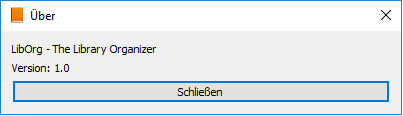
\includegraphics[width=0.60\textwidth]{figures/AboutDialog.png}
	\caption{AboutDialog}
	\label{fig:AboutDialog}
\end{figure}

\textbf{BaseException}\\
Die Klasse BaseException stellt eine Fehlerklasse dar. Im Gegensatz zur Qt-Variante für Exceptions (QException) wird der Fehlertext im Abbruchsfenster gezeigt.\\
Die Basisklasse von BaseException ist std::exception.\\
Die Klasse enthält folgende Methoden und öffentliche Member:
\begin{description}
	\item[ ] enum ErrorCode: ErrorInCode (100)\\
	Beschreibt den aufgetretenen Fehler in Form eines Codes. Derzeit existieren nur Fehler, die auf Fehler im Quellcode, also die Programmierung, zurückzuführen sind.
  \item[ ] BaseException(ErrorCode code, QString explanation)\\
	Erstellt ein neues BaseException-Fehlerobjekt unter Angabe des Fehlercodes (code) und einer Beschreibung (explanation).
  \item[ ] \~{}BaseException()\\
	Zerstört das Objekt und gibt den Speicherplatz frei.
  \item[ ] const char* what() const noexcept\\
	Diese Methode liefert den Fehlertext des Fehlerobjektes zurück. 
\end{description}

\textbf{ConfigDialog}\\
Die Klasse ConfigDialog dient als Basisklasse für beliebige Dialoge, die mit den Konfigurationsklassen einen Einstellungsdialog bilden können. Die Methoden der Klasse sind:
\begin{description}
	\item[ ] virtual void setModified(bool modified) = 0\\
	Diese virtuelle Methode hat in der Klasse keine Implementierung. Sie muss in der abgeleiteten Klasse implementiert werden und dient dazu, zu markieren, dass sich Werte von Konfigurationen innerhalb des Dialogs geändert haben.
\end{description}

\textbf{ConfigWidget}\\
ConfigWidget stellt ein Widget zur Anzeige und Bearbeitung aller Konfigurationseinträge bereit. Alle Elemente eines Konfigurationsblockes können ein- und ausgeblendet werden.\\
Die Basisklassen sind: QWidget und ConfigObserver.\\
Methoden:
\begin{description}
	\item[ ] explicit ConfigWidget(Config* cfg, ConfigDialog *parentDialog, QWidget *parent = nullptr)\\
	Erzeugt ein neues ConfigWidget. Dabei wird für jeden Eintrag in Config ein entsprechendes Darstellungswidget (configwidgetelement) erstellt. Der Klasse muss der parentDialog sowei ein parent übergeben werden.
  \item[ ] \~{}ConfigWidget()\\
		Zerstört das Widget mit allen untergeorndeten child-Widgets.
  \item[ ] void cfgblockchanged(QString blockname, Action action) noexcept\\
		Mit der Methode wird dem ConfigDialog mitgeteilt, dass sich der Blockname entsprechend der action geändert hat.
  \item[ ] void cfgkeyofblockchanged(QString blockname, QString keyname, Action action) noexcept\\
	Diese Methode dient dazu dem ConfigDialog mitzuteilen, sich sich der Konfigruationseintrag gemäß blockname und keyname entsprechend der action geändert hat.
\end{description}

\textbf{ConfigWidgetElement}\\
Ein ConfigWidgetElement stellt basierend auf dem Konfigurationsschlüssel ein passendes Widget bereit. Die Basisklasse ist QWidget. Die Klasse enthält folgende Methoden:
\begin{description}
	\item[ ] explicit ConfigWidgetElement(QString blockname, QString keyname, Config* cfg, QWidget *parent = nullptr)\\
	Erzeugt basierend auf dem Konfigurationsschlüssel blockname und keyname aus der Config ein entsprechendes Anzeigeelement. Wie üblich, sollte ein parent-Objekt übergeben werden.
   \item[ ] \~{}ConfigWidgetElement()\\
	  Zerstört das Anzeigeelement wieder.
\end{description}

\textbf{SettingsDialog}\\
Die Klasse SettingsDialog stellt einen Dialog zur Anzeige und Bearbeitung von Konfigurationsdateien, siehe Abbildung \ref{fig:SettingsDialog}, dar. Die Klasse ist abgeleitet von QDialog und ConfigDialog. Ihre Methoden sind:
\begin{description}
	\item[ ] explicit SettingsDialog(Config *cfg, QWidget *parent = 0)\\
	Erzeugt einen neuen Dialog unter Übergabe einer Konfigurations (cfg) und eines parents. Der Dialog enthält beim Anzeigen für jeden Konfigurationsschlüssel ein eigenes Widget zu dessen Bearbeitung und Anzeige. Jeder Konfigurationsblock kann eingeklappt werden.
	\item[ ] \~{}SettingsDialog()\\
	Zerstört das Objekt und löscht alle Kindelemente.
	\item[ ] void setModified(bool modified)\\
	Diese Methode musste von ConfigDialog überladen und implementiert werden. Ändert sich ein Konfigurationseintrag, so wird dies am Dialogstitel durch ein * gekennzeichnet. Wird der Dialog nun geschlossen, so wird vorab nachgefragt, ob die Änderungen gespeichert werden sollen.
\end{description}
\begin{figure}[htb]
	\centering
		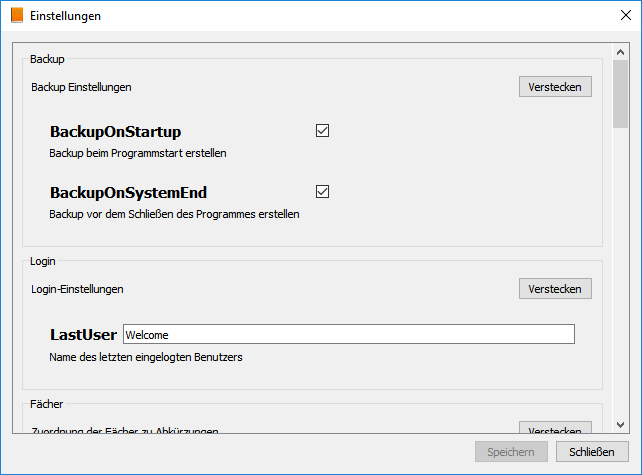
\includegraphics[width=0.70\textwidth]{figures/SettingsDialog.png}
	\caption{SettingsDialog (Beispiel)}
	\label{fig:SettingsDialog}
\end{figure}

\textbf{Licenceplugin}\\
Die Klasse Licenceplugin stellt einen Plugin-Mechanismus zur Anzeige von Lizenztexten bereit. Licenceplugin ist von QObject abgeleitet und besitzt folgende Methoden:
\begin{description}
	\item[ ] static void CreatePlugin()\\
	Erzeugt das Plugin.
  \item[ ] static void DeletePlugin()\\
	Das Plugin wird zerstört.
  \item[ ] static void Add3rdPartyLicence(LicenceItem *item)\\
	Diese Methode hängt eine neue Lizenz (LicenceItem) an das Plugin an.
  \item[ ] static Licenceplugin* Instance()\\
	Liefert die Instanz des Plugins zurück.
  \item[ ] static void ShowLicences(QWidget *parent)\\
	Erzeugt einen Dialog, der alle Lizenzen anzeigt. Dieser Methode wird der parent für den Dialog übergeben.
\end{description}
Licenceplugin ist unter Verwendung des Singelton Patterns implementiert worden, allerdings nicht threadsafe. Aus diesem Grund kann ein Objekt dieser Klasse nur durch die statische Methode CreatePlugin() erzeugt werden.

\textbf{LicenceItem}\\
Die Klasse LicenceItem stellt eine Basisklasse für Lizenzdateien bereit, die in das Licenceplugin eingefügt werden können. Das LicenceItem ist von QObject abgeleitet. Seine Methoden sind:
\begin{description}
	\item[ ] LicenceItem()\\
	Erzeugt ein neues LicenceItem.
  \item[ ] virtual \~{}LicenceItem()\\
	Zerstört das LicenceItem.
  \item[ ] virtual QPushButton* getButton(QWidget* parent)\\
	Erzeugt einen neuen Button für das LicenceItem und gibt diesen zurück. Der parent des Buttons wird auf parent gesetzt.
  \item[ ] virtual QPushButton* getButton()\\
	Liefert den erzeugten Button für das LicenceItem zurück, erstellt einen Button, falls noch keiner erstellt worden ist.
  \item[ ] virtual QWidget* getWidget(QWidget* parent)\\
	Erstellt ein Widget für das LicenceItem und gibt dieses zurück. Das Widget erhält als parent parent.
  \item[ ] virtual QWidget* getWidget()\\
	Liefert das Widget für das LicenceItem zurück, ggf. wird ein neues Widget ohne parent erzeugt.
  \item[ ] virtual void removeWidget()\\
	Zerstört das Widget des LicenceItem und gibt dessen Speicherplatz frei.
\end{description}



		\subsubsection{ExcelReader.dll (DH)}
		In diesem Abschnitt wird die Library zum Auslesen von Excel-Dateien vorgestellt. Leider stellt Qt hierfür keine Funktionalität bereit, verweist jedoch auf die Library FreeXL. Ihr Source-Code kann unter www.gaia-gis.it/fossil/freexl/index heruntergeladen werden und beinhaltet Funktionen, geschrieben in C. Zur besseren Handhabung des Codes ist eine Klasse in C++ geschrieben worden: ExcelReader. Diese Klasse dient als Wrapper um die C-Funktionen von FreeXL.\bigskip \\
Die Klasse ExcelReader enthält folgende Methoden:
\begin{description}
	\item[ ] ExcelReader()\\
	Erzeugt ein neues Objekt von ExcelReader.
  \item[ ] int openXLS(QString filename) noexcept\\
	Liest die übergebene Datei (Achtung nur .xls, altes Excel-Format) ein. Liefert bei erfolgreichem Öffnen XLSFREE\_OK zurück.
  \item[ ]  int close() noexcept\\
	Schließt die mit openXLS geöffnete Datei wieder, liefert XLSFREE\_OK bei erfolgreichem Schließen zurück.
  \item[ ]  unsigned int worksheeds() noexcept\\
	Liefert die Anzahl der Worksheeds der geöffneten Excel-Datei zurück.
  \item[ ]  int selectworksheed(unsigned int index) noexcept\\
	Selektiert das mit index ausgewählte Worksheed und liefert XLSFREE\_OK zurück, wenn das Worksheed selektiert werden konnte.
  \item[ ]  unsigned int rowsofselectedsheet()\\
	Liefert die Anzahl der Zeilen des selektierten Worksheeds zurück.
  \item[ ]  unsigned int columnsofselectedsheet()\\
	Liefert die Anzahl der Spalten des selektierten Worksheeds zurück.
  \item[ ]  FreeXL\_CellValue getCellValue(unsigned int row, unsigned short column)\\
	Liefert den Wert zurück, der sich in der Zeile row und der Spalte column befindet.
  \item[ ]  \~ExcelReader()\\
	Zerstört das ExcelReader-Objekt und gibt verwendeten Speicherplatz frei.
\end{description}
Der ExcelReader und der Source-Code von FreeXL befindet sich in der dll ExcelReader.dll.

		\subsubsection{Hauptanwendung (JH)}
		\textbf{Icon-Files}\\
Für die Anwendung wird zum einen eine Icon-Datei für die Dialoge und Fenster benötigt. Hierzu ist eine .png-Bilddatei erstellt worden, da das Qt-Framework dieses Format für alle Icons innerhalb der Anwendung unterstützt.\\
Für ein Icon für die exe-Datei kann jedoch keine .png-Bilddatei verwendet werden, sondern es muss eine .ico-Datei erstellt werden. Als Programm zum Erstellen der ico-Datei ist Gimp gemäß \cite{CreateICO} verwendet worden. Das Tutorial beschreibt den exakten Weg zum Erstellen aller Bildformate für Windows. Die ico-Datei muss anschließend im Qt-Projekt konfiguriert werden. \cite{SetICO} benennt die notwendigen Schritte: Im Projekt-Ordner muss eine .rc-Datei mit dem Inhalt "`IDI\_ICON1 ICON    DISCARDABLE "nameOfIco.ico""' angelegt werden. Zum Abschluss muss in der .pro-Datei des Projektes die Zeile "`RC\_FILE = myapp.rc"' eingefügt werden.\bigskip \\

\textbf{BookModel}\\
Das BookModel, abgleitet von QAbstractTableModel, enthält alle Buchdaten. Die Daten werden aus der Datenbank gelesen und zeilenweise im Model abgespeichert. Folgende Methoden sind reimplementiert:
\begin{description}
	\item[ ] explicit BookModel(BookTable *table, LendingTable *ltable, QObject *parent = nullptr)\\
	Initialisiert das Model mit den notwendigen Informationen, dies sind ein Verweis auf die BookTable und LendingTable der Datenbank-API sowie ein optionaler parent.
  \item[ ] \~{}BookModel()\\
	Zerstört das Model und löscht alle Daten in ihm aus dem Speicher.
  \item[ ] QVariant headerData(int section, Qt::Orientation orientation, int role = Qt::DisplayRole) const override\\
	Liefert die Headerinformationen zurück. Diese sind: Titel, Untertitel, ISBN, Jahrgangsstufe, Fach und verfügbare Anzahl eines Buches.
  \item[ ] int rowCount(const QModelIndex \&parent = QModelIndex()) const override//
	Liefert die Anzahl der Zeilen, gleich die Anzahl der Bücher im Model.
  \item[ ] int columnCount(const QModelIndex \&parent = QModelIndex()) const override\\
	Das Model besitzt sechs Spalten, diese wird von dieser Methode zurückgegeben.
  \item[ ] QVariant data(const QModelIndex \&index, int role = Qt::DisplayRole) const override\\
	Liefert die Information pro Zeile und Spalte (dem Index) pro Role zurück. Diese Informationen entsprechen dem jeweiligen Header.
  \item[ ] bool removeRows(int row, int count, const QModelIndex \&parent = QModelIndex()) override\\
	Löscht das Buch aus der Datenbank und dem Model. Vorab wird überprüft, ob das Buch noch ausgeliehen ist, indem Fall darf und wird das Buch nicht gelöscht aber eine Warnung angezeigt.
  \item[ ] void reset()\\
	Setzt das Model zurück.
  \item[ ] void search(QString searchstring)\\
  Filtert anhand des searchstring nach passenden Büchern. Alle nicht passenden Bücher werden aus dem Model entfernt.
  \item[ ] BookTable::BookRow* getRow(QModelIndex row)\\
	Mit dieser Methode kann der zu einer Zeile (row) gehörende Bucheintrag zurückgegeben werden. Diese Methode wird benötigt, um eine Buchzeile in einer Maske bearbeiten zu können.
  \item[ ] void updateRow(int row)\\
	Weist die View des Models an, die entsprechende Zeile neu zu laden. Sie wird ebenfalls benötigt, um eine Buchzeile in einer Maske bearbeiten zu können.
  \item[ ] void addRow(BookTable::BookRow * newRow)\\
	Durch den Aufruf dieser Methode kann dem Model eine neue Buchzeile (newRow) hinzugefügt werden.	
\end{description}

\textbf{BookWidget}\\
Das BookWidget, siehe Abbildung \ref{fig:BookWidget}, kann in ein Fenster eingebettet werden. Es besitzt ein Objekt der Klasse BookModel, um die darin enthaltenen Bücher anzuzeigen. BookWidget ist von QWidget abgeleitet. Seine Methoden sind:
\begin{description}
	\item[ ] explicit BookWidget(Dataset *set, QWidget *parent = 0)\\
	Konstruiert eine neue Instanz von BookWidget, dazu muss ihm das Dataset und optional ein parent übergeben werden. 
  \item[ ] \~{}BookWidget()\\
	Zerstört das Objekt und gibt den Speicherplatz wieder frei.
	\item[ ] Signal: void closewidget()\\
	Dieses Signal wird emittiert, wenn das BookWidget verworfen werden soll.
\end{description}
Das BookWidget erlaubt es, Bücher anzuzeigen, diese zu filtern, Bücher hinzuzufügen und zu löschen. Außerdem können Bücher mittels einer Maske bearbeitet werden.
\begin{figure}[htb]
	\centering
		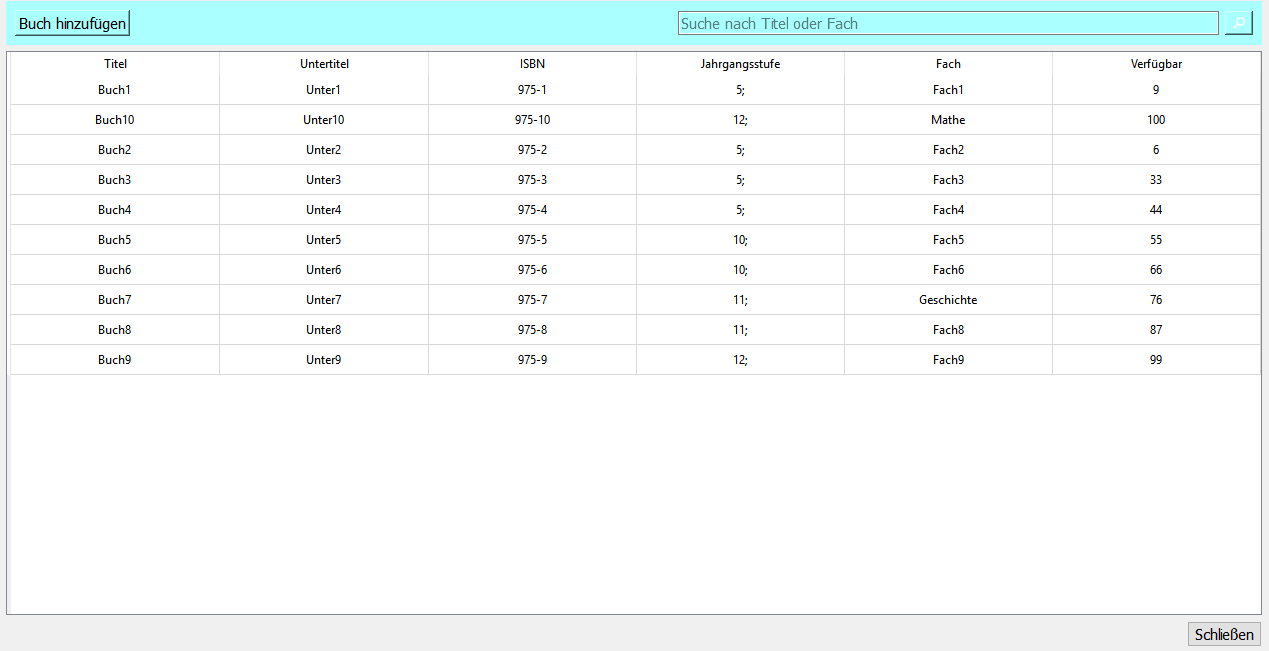
\includegraphics[width=0.70\textwidth]{figures/BookWidget.PNG}
	\caption{BookWidget}
	\label{fig:BookWidget}
\end{figure}
 \bigskip \\

\textbf{BookMask}\\
Die BookMask-Klasse beinhaltet den Dialog zur Bearbeitung und Neuanlage von Büchern. Er ist in Abbildung \ref{fig:BookMask} abgebildet. Ihre Basisklasse ist QDialog. Die öffentlichen Methoden sind:
\begin{description}
	\item[ ] explicit BookMask(BookTable *table, QWidget *parent = 0)\\
	Erzeugt die Büchermaske. Das Objekt benötigt einen Pointer auf die BookTable des Dataset und optional einen parent für den Dialog.
  \item[ ] \~{}BookMask()\\
	Zerstört das Objekt und gibt den Speicher wieder frei.	
  \item[ ] BookTable::BookRow* getInsertedBookRow()\\
	Liefert die neu erstellte Zeile zurück.
  \item[ ] void setBookRow(BookTable::BookRow* row)\\
	Übergibt eine Bücherzeile an die Büchermaske zur Bearbeitung und Anzeige.
\end{description}
\begin{figure}[htb]
	\centering
		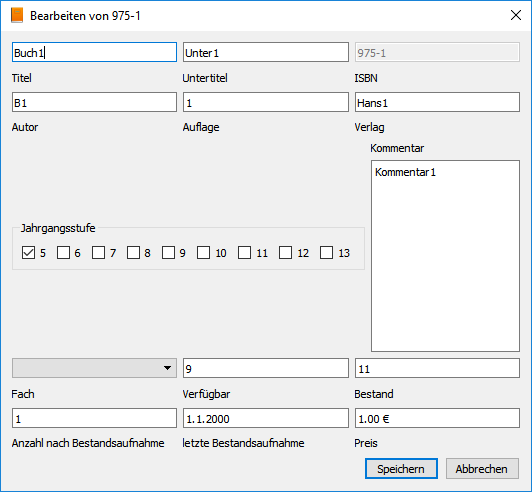
\includegraphics[width=0.60\textwidth]{figures/BookMask.png}
	\caption{Büchermaske}
	\label{fig:BookMask}
\end{figure}

\textbf{DamageDialog}\\
Der DamageDialog dient zur Abfrage, ob ein Buch beschädigt ist. Ein Beispiel des Dialogs ist in Abbildung \ref{fig:DamageDialog} dargestellt. Der Dialog erbt von QDialog, weitere Methoden sind:
\begin{description}
	\item[ ] explicit DamageDialog(QString forename, QString surname, QString booktitle, QWidget *parent = 0)\\
	Erzeugt ein Objekt von DamageDialog unter Angabe eines Vornamens, eines Nachnahmens und eines Buchtitels. Diese Informationen werden im Dialog angezeigt.
	\item[ ] \~{}DamageDialog()\\
	Zerstört das Objekt und gibt den Speicherplatz frei.	
  \item[ ] QString getDamage()\\
	Liefert den eingetragenen Schaden zurück. Wird kein Schaden vergeben, so wird ein leerer String zurückgegeben.
\end{description}
\begin{figure}[htb]
	\centering
		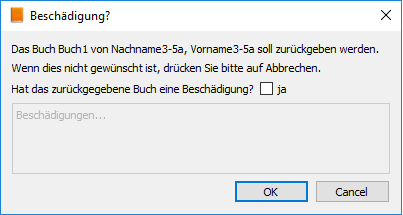
\includegraphics[width=0.60\textwidth]{figures/DamageDialog.png}
	\caption{DamageDialog}
	\label{fig:DamageDialog}
\end{figure} 

\textbf{DamagesWidget}\\
Das DamagesWidget zeigt alle Rückgaben des jeweiligen Schülers in Form eines Baumes an. Durch den "`Begleichen"'-Button wird der Schaden aus der Rückgabe entfernt. Das Widget ist in Abbildung \ref{fig:DamagesWidget} abgebildet.
\begin{description}
	\item[ ] explicit DamagesWidget(Dataset* set, QWidget *parent = 0)\\
	Erzeugt ein neues Objekt von DamagesWidget, dabei muss ein Dataset und optional ein parent übergeben werden.
  \item[ ] \~{}DamagesWidget()\\
	Zerstört das Objekt und gibt den Speicher frei.
	\item[ ] Signal: closewidget()\\
	Das Signal wird emittiert, wenn das Widget aus seinem parent entfernt werden soll.
\end{description}
\begin{figure}[htb]
	\centering
		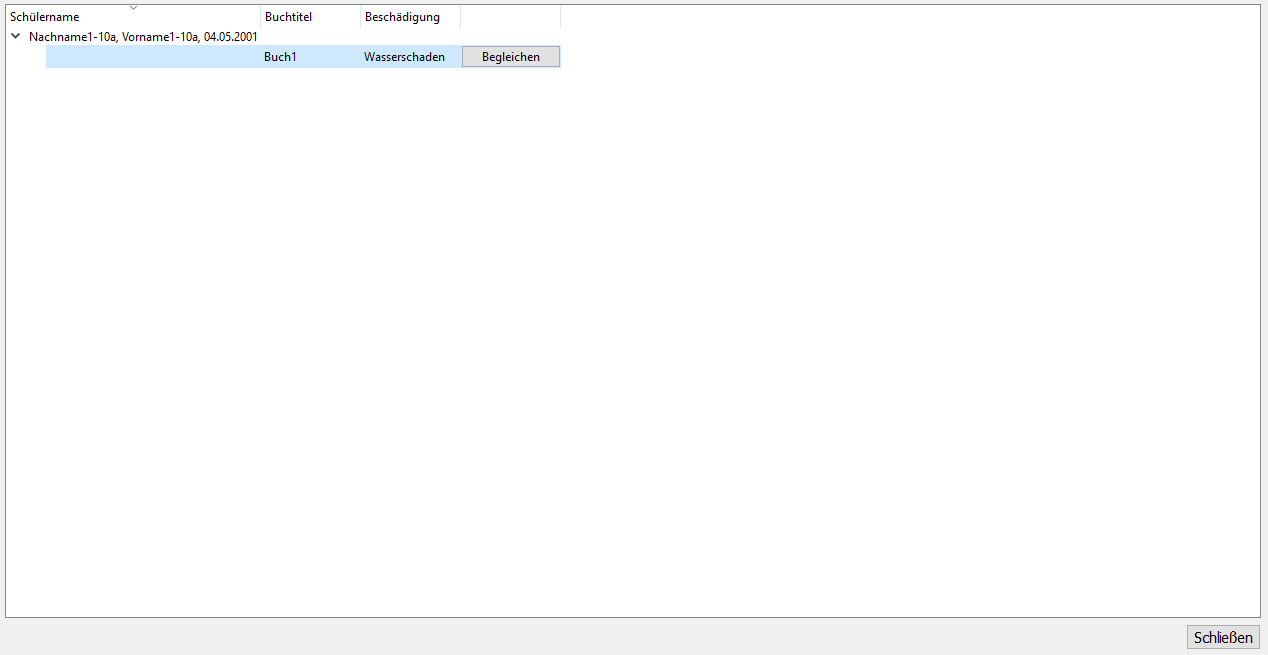
\includegraphics[width=0.70\textwidth]{figures/DamagesWidget.PNG}
	\caption{DamagesWidget}
	\label{fig:DamagesWidget}
\end{figure}

\textbf{StudentModel}\\
Das StudentModel enthält alle Informationen von Schülern. Es greift über die Datenbank-API auf die Informationen der Schülerdatenbank zu. Das Model ist von QAbstractTableModel abgeleitet, folgende Methoden sind implementiert:
\begin{description}
	\item[ ] StudentModel(StudentTable* stable, QObject* parent = 0)\\
	Konstruiert ein neues Objekt von StudentModel, das einen Pointer auf die StudentTable des Dataset erhält sowie optional einen parent.
  \item[ ] \~{}StudentModel()\\
	Zerstört das Objekt und löscht alle Daten aus dem Model.
	\item[ ] int rowCount(const QModelIndex \&parent) const\\
	Liefert die Anzahl der Schüler, also die Anzahl der Zeilen, zurück.
  \item[ ] int columnCount(const QModelIndex \&parent) const\\
	Gibt die Anzahl der Spalten (vier) zurück.
  \item[ ] QVariant data(const QModelIndex \&index, int role) const\\
	Es werden die einzelnen Informationen aus dem Model entsprechend dem index und der role herausgelesen.
  \item[ ] QVariant headerData(int section, Qt::Orientation orientation, int role) const\\
	Liefert die Headerinformationen pro Spalte: Name, Geburtsdatum und Klasse. Die vierte Spalte erhält keinen Header.
  \item[ ] void selectClass(QString className)\\
	Wählt eine Klasse aus. Dabei werden alle Schüler aus dem Model entfernt, die nicht in die gewählte Klasse gehören.
  \item[ ] void search(QString searchstring)\\
	Filtert gemäß des searchstring die Schüler aus dem Model (nicht passende Einträge werden aus dem Model entfernt).
	\item[ ] void deleteStudent(int row)\\
	Löscht den Schüler, der sich an der Stelle row befindet aus dem Model.
  \item[ ] void reset()\\
	Setzt das Model zurück.
  \item[ ] StudentTable::StudentRow* getStudent(QModelIndex index)\\
	Liefert die StudentRow aus dem Model an der Stelle index zurück, so dass die Zeile bearbeitet werden kann. Der Pointer darf nicht gelöscht werden!
  \item[ ] StudentTable::StudentRow* getStudent(int row)\\
	Gleiches Ergebnis wie bei getStudent(QModelIndex index) nur unter Angabe der Zeilennummer.
  \item[ ] void updateRow(int row)\\
	Die Zeile an der Position row wird aktualisiert. Diese Methode muss aufgerufen werden, wenn eine mit getStudent() erhaltene Zeile bearbeitet wurde. Das Model aktualisiert hierdurch die View.
  \item[ ] void addStudent(StudentTable::StudentRow* newRow)\\
	Ein neu angelegter Schüler wird in das Model eingefügt.
\end{description}
    
\textbf{StudentWidget}\\
Das StudentWidget zeigt mittels einer TableView die Einträge im StudentModel an, siehe Abbildung \ref{fig:StudentWidget}. Das Widget erlaubt es eine Klasse auszuwählen und damit alle Schüler dieser Klasse anzuzeigen. Zudem kann nach Schülern gefiltert werden. StudentWidget ist abgeleitet von QWidget. Die Methoden sind:
\begin{description}
	\item[ ] explicit StudentWidget(Dataset* set, UserPermissions permission, QWidget *parent = 0)\\
	Erzeugt ein StudentWidget-Objekt unter Übergabe eines Pointers auf das Dataset, UserPermissions und optional ein parent-Objekt.
  \item[ ] \~{}StudentWidget()\\
	Zerstört das Widget wieder und gibt den Speicherplatz frei.
	\item[ ] void closewidget()\\
	Das Signal wird ausgegeben, wenn das Widget aus dem parent-Element entfernt werden soll.	
\end{description}
\begin{figure}[htb]
	\centering
		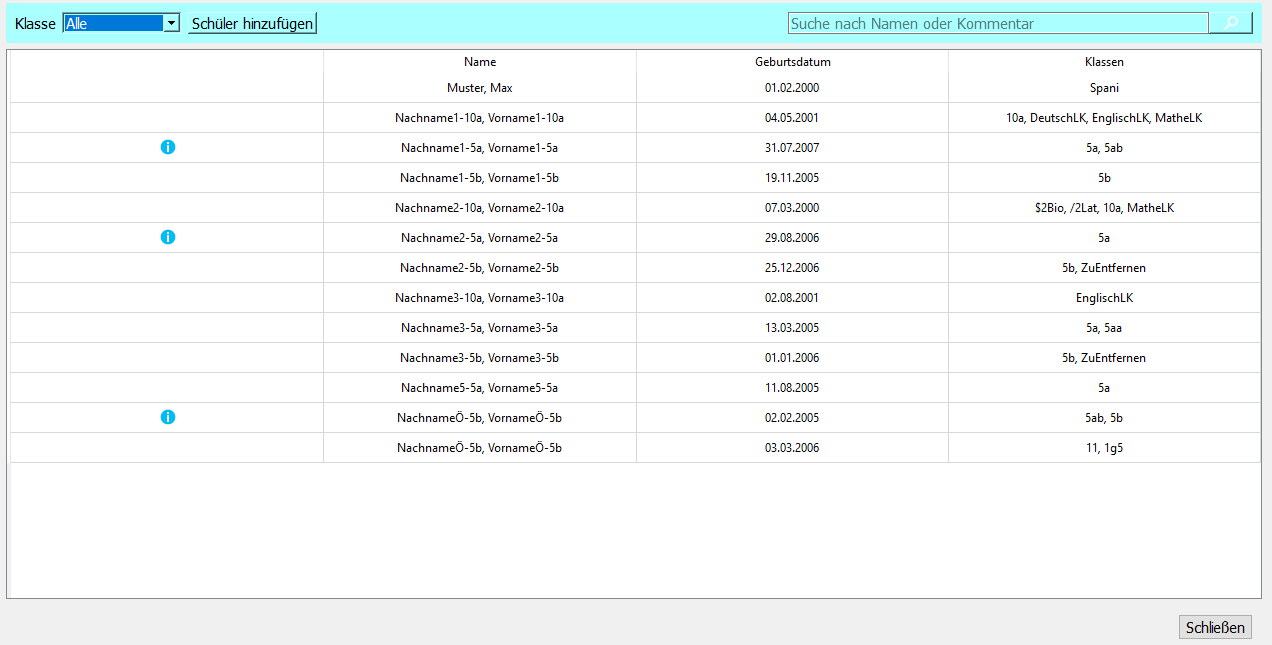
\includegraphics[width=0.60\textwidth]{figures/StudentWidget.PNG}
	\caption{StudentWidget}
	\label{fig:StudentWidget}
\end{figure}

\textbf{StudentMask}\\
Die StudentMask stellt eine Maske zur Bearbeitung bzw. Neuanlage eines Schülers dar. Die Eintragungen werden überwacht. Die Maske ist in Abbildung \ref{fig:StudentMask} dargestellt. Die Basisklasse ist QDialog, weitere Methoden sind:
\begin{description}
	\item[ ] explicit StudentMask(Dataset* set, QWidget* parent = 0)\\
	Erzeugt ein neues Objekt der StudentMask-Klasse. Es muss ein Pointer auf das Dataset und optional ein parent übergeben werden.
   \item[ ] \~{}StudentMask()\\
	Zerstört das Objekt.
   \item[ ] void selectStudent(StudentTable::StudentRow *row)\\
	 Überträgt den übergebenen Schüler (row) auf die Schülermaske, so dass diese row bearbeitet werden kann (die Änderungen werden beim Akzeptieren des Dialogs direkt in die row geschrieben).
   \item[ ] StudentTable::StudentRow* getNewStudent()\\
	Liefert den neu erzeugten Schüler zurück.
\end{description}
\begin{figure}[htb]
	\centering
		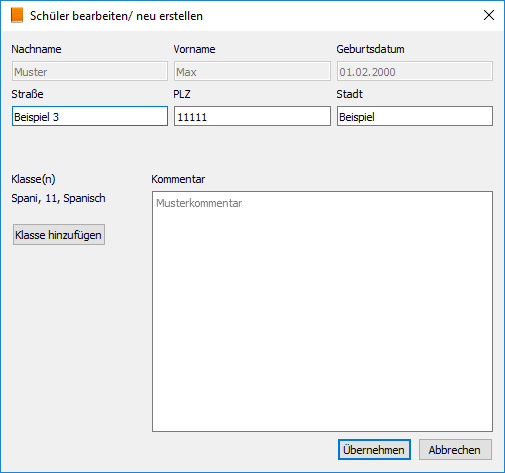
\includegraphics[width=0.60\textwidth]{figures/StudentMask.png}
	\caption{StudentMask}
	\label{fig:StudentMask}
\end{figure}

\textbf{AddClass}\\
AddClass stellt eine Maske zum Hinzufügen einer neuen Klasse dar. Die Eintragungen werden überwacht. 
\begin{description}
	\item[ ] explicit addclass(QWidget *parent = 0)\\
	Erzeugt ein neues Objekt der AddClass-Klasse. Es kann optional ein Pointer übergeben werden.
	\item[ ] ~addclass()\\
	Destruktor, zerstört das Objekt.
	\item[] ClassTable::ClassRow getNewClass()\\
	Liefert die neu erzeugte Klasse zurück.
\end{description}

\textbf{AddUserDialog}\\
AddUserDialog stellt den Dialog zum Hinzufügen eines neuen Benutzers bereit. Die Eintragungen werden überwacht. 
\begin{description}
	\item[] explicit adduserdialog(Dataset* set, QWidget *parent = 0)\\
	Erzeugt ein neues Objekt der AddUserDialog-Klasse. Es muss ein Pointer auf das verwendete Dataset und optional ein Parent übergeben werden.
	\item[] ~adduserdialog()\\
	Destruktor, zerstört das Objekt.
  	\item[] void selectUser(QString user, UserTable::UserRow* row)\\
	Füllt die gegebenen Benutzerdaten in den Benutzerdialog, um ihn zu bearbeiten. Benötigt den Namen des momentanen Benutzers, sowie die UserRow aus der UserTable der Datenbank.
  	\item[] UserTable::UserRow* getReturnUser()\\
	Liefert den neuen, bzw. den geänderten, Benutzer zurück.
\end{description}

\textbf{Dataset}\\
Das Dataset stellt die Daten dar, mit denen das Programm arbeitet und enthält daher die Daten, der Datenbank.
\begin{description}
	\item[] Dataset() \\
	Erzeugt eine neues Dataset Objekt.
	\item[] virtual ~Dataset() \\
	Destruktor, zerstört das Objekt.
  	\item[] UserTable mUserTable \\
  	Bildet die Benutzertabelle der Datenbank ab.
  	\item[] ClassTable mClassTable \\
  	Bildet die Klassentabelle der Datenbank ab.
  	\item[] StudentClassTable mStudentClassTable \\
  	Bildet die Student-Klassentabelle der Datenbank ab.
  	\item[] StudentTable mStudentTable \\
  	Bildet die Schülertabelle der Datenbank ab.
  	\item[] BookTable mBookTable \\
  	Bildet die Büchertabelle der Datenbank ab.
  	\item[] GiveBackTable mGiveBackTable \\
  	Bildet die Rückgabetabelle der Datenbank ab.
  	\item[] LendingTable mLendTable \\
  	Bildet die Ausleihtabelle der Datenbank ab.
\end{description}

\textbf{CheckBoxDelegate}\\
Erweitert ein TableWidget um eine klickbare Checkbox.
\begin{description}
	\item[ ] CheckBoxDelegate(QObject *parent = 0) \\
	Erzeugt ein neues CheckBoxDelegate Objekt. Optional kann ein Parent übergeben werden.
  	\item[ ] void paint(QPainter *painter, const QStyleOptionViewItem \&option, const QModelIndex \&index) const \\
	Rendert den Delegate für das übergebene Item, an Position index, mit den übergeben Optionen. Dafür wird ein painter, sowie Styleoptionen und der index übergeben. 
  	\item[ ] virtual bool editorEvent(QEvent *event, QAbstractItemModel *model, const QStyleOptionViewItem \&option, const QModelIndex \&index) \\
  	Wird aufgerufen wenn ein Event auf dem Item des Delegate aufgerufen wird. Es wird das auslösende Event, das Model, das QStyleOptionViewItem, sowie der Index des Items übergeben.
\end{description}

\textbf{LendDelegate}\\
Erweitert ein TableWidget um eine Checkbox, sowie einen Plus- und Minusbutton. Wird für die Ausleihfunktionalität benötigt. 
\begin{description}
	\item[ ] LendDelegate(QObject *parent = 0) \\
	Erzeugt ein neues LendDelegate Objekt. Optional kann ein Parent übergeben werden.
  	\item[ ] void paint(QPainter *painter, const QStyleOptionViewItem \&option, const QModelIndex \&index) const \\
	Rendert den Delegate für das übergebene Item, an Position index, mit den übergeben Optionen. Dafür wird ein painter, sowie Styleoptionen und der index übergeben.
  	\item[ ] virtual bool editorEvent(QEvent *event, QAbstractItemModel *model, const QStyleOptionViewItem \&option, const QModelIndex \&index) \\
  	Wird aufgerufen wenn ein Event auf dem Item des Delegate aufgerufen wird. Es wird das auslösende Event, das Model, das QStyleOptionViewItem, sowie der Index des Items übergeben.
\end{description}	

\textbf{SelectClass}\\
SelectClass stellt einen Dialog bereit um Klassen auszuwählen.
\begin{description}
	\item[ ] explicit SelectClass(Dataset* set, QList<ClassTable::ClassRow> classes, QWidget *parent = 0) \\
	Erzeugt ein neues SelectClass Objekt, dafür wird das Dataset, sowie eine Liste der Klassen und optional ein parent übergeben.
  	\item[ ] ~SelectClass() \\
	Destruktor, zerstört das Objekt.
  	\item[ ] QList<ClassTable::ClassRow> getSelectedClasses() \\
	Gibt eine Liste der im Dialog ausgewählten Klassen zurück.
	\item[ ] void close() \\
	Schließt den Dialog.
\end{description}

\textbf{UserManagementDialog}\\
UserManagementDialog stellt einen Dialog bereit, um die Benutzer der LibOrg Software zu verwalten.
\begin{description}
	\item[ ] explicit usermanagementdialog(Dataset *set, QString currentUser, QWidget *parent = 0) \\
	Erzeugt ein neues UserManagementDialog Objekt, hierfür wird das Dataset, sowie der Name des momentan angemeldeten Benutzers und, optional, ein Parent übergeben.
  	\item[ ] ~usermanagementdialog() \\
	Destruktor, zerstört das Objekt.
\end{description}

\textbf{UserModel (UserManagementDialog)}\\
UserModel stellt das Model bereit um den TableView im UserManagementDialog mit Daten zu füllen.
\begin{description}
	\item[ ] explicit UserModel(UserTable *table, QObject *parent = nullptr) \\
	Erzeugt einn neues UserModel Objekt, hierfür wird die Usertable und optional ein parent übergeben.
  	\item[ ] ~UserModel() \\
  	Destruktor, zerstört das Objekt.
	\item[ ] QVariant headerData(int section, Qt::Orientation orientation, int role = Qt::DisplayRole) const override \\
  	Gibt die Daten, die in den Header des Models gehören, zurück. Hierfür wird eine Section eine orientation und eine Role übergeben.
	\item[ ] int rowCount(const QModelIndex \&parent = QModelIndex()) const override \\
  	Gibt die Anzahl der Reihen zurück. Hierfür wird ein Index übergeben.
	\item[ ] int columnCount(const QModelIndex \&parent = QModelIndex()) const override \\
  	Gibt die Anzahl der Spalten zurück. Hierfür wird ein Index übergeben.
	\item[ ] QVariant data(const QModelIndex \&index, int role = Qt::DisplayRole) const override \\
  	Gibt die Daten für das Model zurück. Hierfür wird ein Index und eine Role übergeben.
	\item[ ] bool removeRows(int row, int count, const QModelIndex \&parent = QModelIndex()) override \\
	Löscht Reihen aus dem Model. Es wird die Startrow sowie die Anzahl der zu löschenden Reihen und ein Index übergeben.
	\item[ ] void reset() \\
  	Resettet das Model.
	\item[ ] void fillModel() \\
	Füllt das Model mit den zugehörigen Daten.
	\item[ ] UserTable::UserRow* getRow(int row) \\
  	Gibt die Reihe an der Stelle row zurück.
	\item[ ] void updateRow(UserTable::UserRow * updatedRow, int row) \\
  	Aktualisiert eine Reihe, hierfür wird der Index der Reihe sowie die neuen Daten, als UserRow, übergeben.
	\item[ ] void addRow(UserTable::UserRow * newRow) \\
	Fügt eine Reihe zum Model hinzu. Es wird die Reihe, welche hinzugefügt werden soll, übergeben.
\end{description}

\textbf{ClassModel}\\
Stellt das Model für einen TableView der Klassen bereit.
\begin{description}
	\item[ ] ClassModel(Dataset* set, QObject* parent = 0) \\
	Erzeugt ein neues ClassModel Objekt, hierfür wird das Dataset und optional ein parent übergeben.
  	\item[ ] ~ClassModel() \\	
	Destruktor, zerstört das Objekt.
  	\item[ ] int rowCount(const QModelIndex \&parent) const \\
	Gibt die Anzahl der Reihen zurück. Hierfür wird der Index des Models übergeben.
  	\item[ ] int columnCount(const QModelIndex \&parent) const \\
	Gibt die Anzahl der Spalten zurück, hierfür wird der Index des Models übergeben.
  	\item[ ] void initialize() \\
	Initialisiert das Model.
  	\item[ ] QVariant data(const QModelIndex \&index, int role) const \\
	Gibt die Daten des Models mit dem Index und der Role zurück.
 	\item[ ] bool setData(const QModelIndex \&index, const QVariant \&value, int role) \\
	Setzt die Daten des Models. Es wir der Index des Models sowie die Values und die Role übergeben.
 	\item[ ] QVariant headerData(int section, Qt::Orientation orientation, int role) const \\
	Gibt die Daten für den Header zurück. Hierür wird die Sektion, die Orietierung und die Role übergeben.
  	\item[ ] Qt::ItemFlags flags(const QModelIndex \&index) const \\
	Gibt die gesetzten Flags für ein Model mit dem Index index zurück.
  	\item[ ] QList<ClassTable::ClassRow> getSelectedClasses() \\
	Gibt die momentan ausgewählten Klassen zurück.
  	\item[ ] void addClass(ClassTable::ClassRow newClass) \\
	Fügt eine neue Klasse zum Model hinzu. Hierfür wird die neue Klasse übergeben.
  	\item[ ] void selectClasses(QList<ClassTable::ClassRow> toSelectClasses) \\
	Wird aufgerufen wenn bestimmte Klassen ausgewählt werden sollen. Hierfür werden die auszuwählenden Klassen übergeben.
  	\item[ ] void reset() \\
	Resettet das Model.
  	\item[ ] void fill() \\
	Füllt das Model mit Daten.
\end{description}

\textbf{BookingWidget}\\
Stelllt das Widget für die Bücher bereit.
\begin{description}
	\item[ ] explicit BookWidget(Dataset *set, QWidget *parent = 0) \\
	Erzeugt ein neues BookWidget Objekt, hierfür wird das Dataset und optional ein parent übergeben.
  	\item[ ] ~BookWidget() \\
	Destruktor, zerstört das Objekt.
	\item[ ] void closewidget() \\
	Beendet das Widget.
\end{description}

\textbf{SingleBookingDialog}\\
Stellt den Dialog für eine Ausleihe eines Buches an einen Schüler bereit.
\begin{description}	
    \item[ ] explicit ShortBookModel(StudentTable::StudentRow *row, StudentTable* stable, BookTable* btable, LendingTable* ltable, QWidget *parent = nullptr); \\
    Erzeugt ein neues ShortBookModel Objekt. Hierfür wird die Studentrow des Schülers, die Studenttable, die Booktable, die Lendingtable, sowie optional ein parent übergeben.
    \item[ ] ~ShortBookModel(); \\
    Destruktor, zerstört das Objekt.
    \item[ ] int rowCount(const QModelIndex \&parent = QModelIndex()) const override; \\
    Gibt die Anzahl der Reihen zurück, hierfür wird der Index des Models übergeben.
    \item[ ] int columnCount(const QModelIndex \&parent = QModelIndex()) const override; \\
    Gibt die Anzahl der Spalten zurück, hierfür wird der Index des Models übergeben.
    \item[ ] QVariant headerData(int section, Qt::Orientation orientation, int role) const; \\
    Gibt die Daten für den Header zurück. Es wird die Section, die Orientation, sowie die Role übergeben.
    \item[ ] QVariant data(const QModelIndex \&index, int role = Qt::DisplayRole) const override; \\
    Gibt die Daten für das Model zurück. Hierfür wird eine Index und eine Role übergeben.
    \item[ ] bool setData(const QModelIndex \&index, const QVariant \&value, int role); \\
    Setzt die Daten des Models. Es wir der Index des Models sowie die Values und die Role übergeben.
    \item[ ] Qt::ItemFlags flags(const QModelIndex \&index) const; \\
    Gibt die gesetzten Flags für ein Model mit dem Index index zurück.
    \item[ ] void select(option option); \\
    Wird aufgerufen, wenn sich die ausgewählte Option ändert. Hierfür wird die option übergeben.
    \item[ ] void setHolidayLending(bool value); \\
    Setzt eine Ausleihe auf Ferienausleihe. Es wird der zu setztende boolean Wert übergeben.
\end{description}

\textbf{StudentLendModel}\\
Stellt das Model für einen TableView, welcher die Ausleihen von Schülern darstellt, bereit.
\begin{description}
    \item[ ] StudentLendModel(StudentTable* stable, BookTable* btable, LendingTable* ltable, QFontMetrics font, QObject * parent = 0); \\
    Erzeugt ein neues StudentLendModel Objekt. Hierfür wird die Studenttable, die Booktable, die Lendingtable, ein Font und optional ein parent übergeben.
    \item[ ] ~StudentLendModel(); \\
    Destruktor, zerstört das Objekt.
    \item[ ] int rowCount(const QModelIndex \&parent) const; \\
    Gibt die Anzahl der Reihen zurück, hierfür wird der Index des Models übergeben.
    \item[ ] int columnCount(const QModelIndex \&parent) const; \\
    Gibt die Anzahl der Spalten zurück, hierfür wird der Index des Models übergeben.
    \item[ ] QVariant data(const QModelIndex \&index, int role) const; \\
    Gibt die Daten für das Model zurück. Hierfür wird ein Index und eine Role übergeben.
    \item[ ] QVariant headerData(int section, Qt::Orientation orientation, int role) const; \\
    Gibt die Daten für den Header zurück. Es wird die Section, die Orientation, sowie die Role übergeben.
    \item[ ] bool setData(const QModelIndex \&index, const QVariant \&value, int role); \\
    Setzt die Daten des Models. Es wir der Index des Models sowie die Values und die Role übergeben.
    \item[ ] Qt::ItemFlags flags(const QModelIndex \&index) const; \\
    Gibt die gesetzten Flags für ein Model mit dem Index index zurück.
    \item[ ] bool setHeaderData(int section, Qt::Orientation orientation, const QVariant \&value, int role); \\
    Setzt die Daten für den Header. Es wir die section, die orientation, der neue value sowie die role übergeben.
    \item[ ] void selectClass(QString classname, int grade, QString subject, BookOption mOption); \\
    Wird aufgerufen wenn eine neue Klasse ausgewählt wird, dabei wird der classname, die grade, das fach und eine bookoption übergeben.
    \item[ ] void selectBookOptions(BookOption option); \\
    Wird aufgerufen wenn sich die bookoption ändert. Hierfür wird die neue Bookoption übergeben.
    \item[ ] void reset(); \\
    Resettet das Model.
    \item[ ] void setDialogParent(QWidget *parent); \\
    Setzt den parent des Dialogs auf den übergebenen parent.
   	\item[ ] void searchInBooks(QString searchString, BookOption mOption); \\
   	Führt eine Suche in den Büchern des Models durch. Hierfür wird der searchstring, sowie die momentane bookoption übergeben.
    \item[ ] StudentTable::StudentRow* getStudent(QModelIndex index); \\
   	Gibt den Schüler an der Stelle index zurück.
\end{description}

\textbf{OpenLendings}\\
Stellt den Dialog, um die Ausleihen eines Schülers anzuzeigen, bereit.
\begin{description}
	\item[ ] LendBooksModel(Dataset *set, QObject* parent); \\
	Erzeugt ein neues LendBookModel Objekt, hierfür wird das Dataset und optional ein parent übergeben.
    \item[ ] ~LendBooksModel(); \\
    Destruktor, zerstört das Objekt.
    \item[ ] void selectOption(QString option); \\
    Wird aufgerufen, wenn sich die Bookoption ändert, es wird die neue Option als String übergeben.
    \item[ ] StudentTable::StudentRow* getStudent(QModelIndex index); \\
    Gibt den Schüler an der Stelle index zurück.
    \item[ ] void updateRow(QModelIndex index); \\
    Aktualisiert die Reihe an der Stelle index.
    \item[ ] int rowCount(const QModelIndex \&parent) const; \\
    Gibt die Anzahl der Reihen zurück, hierfür wird der Index des Models übergeben.
    \item[ ] int columnCount(const QModelIndex \&parent) const; \\
    Gibt die Anzahl der Spalten zurück, hierfür wird der Index des Models übergeben.
    \item[ ] QVariant data(const QModelIndex \&index, int role) const; \\
    Gibt die Daten für das Model zurück. Hierfür wird eine Index und eine Role übergeben.
    \item[ ] QVariant headerData(int section, Qt::Orientation orientation, int role) const; \\
    Gibt die Daten für den Header zurück. Es wird die Section, die Orientation, sowie die Role übergeben.
    \item[ ] bool setData(const QModelIndex \&index, const QVariant \&value, int role); \\
    Setzt die Daten für das Model. Es wird der index, das zu setzende value und die role übergeben.
    \item[ ] Qt::ItemFlags flags(const QModelIndex \&index) const; \\
	Gibt die gesetzten Flags für ein Model mit dem Index index zurück.
\end{description}


\textbf{MainWindow}  \\
Das MainWindow, siehe Abbildung \ref{fig:MainWindow}, stellt das Hauptfenster bzw. die Hauptanwendung dar. Von ihm aus können alle Funktionen der Software ausgeführt werden. Aus diesem Grund werden nicht die öffentlichen Methoden sondern alle anderen Methoden der MainWindow-Klasse vorgestellt:
\begin{description}
	\item[ ] Slot: void rider\_settings\_triggered()\\
	Öffnet den Dialog für die Einstellungen, dabei wird die Klasse SettingsDialog verwendet.
  \item[ ] Slot: void rider\_about\_triggered()\\
	Es wird ein Objekt von AboutDialog angelegt und angezeigt.
  \item[ ] Slot: void rider\_import\_triggered()\\
	Öffnet den Dialog zum Import der ASV- und WinQD-Dateien.
  \item[ ] Slot: void rider\_changeuser\_triggered()\\
	Der Slot wird aufgerufen, wenn der aktuelle Benutzer gewechselt werden soll. Es wird der LoginDialog aufgerufen und bei Eingabe eines neuen Benutzers samt Passwort das Fenster mit den aktuellen Berechtigungen versorgt.
  \item[ ] Slot: void rider\_3rd\_party\_software\_triggered()\\
	Dieser Slot zeigt den Lizenzdialog der Klasse Licenceplugin an.
  \item[ ] Slot: void rider\_lend\_and\_giveback\_triggered()\\
	Platziert ein BookingWidget-Objekt in das vorgesehene leere Widget-Element und zeigt es an. Befand sich vorab ein anderes Objekt in diesem Widget-Element, so wird dieses entfernt.
  \item[ ] Slot: void rider\_books\_triggered()\\
	Leert das Widget-Element und fügt das BookWidget in es ein.
  \item[ ] Slot: void rider\_students\_triggered()\\
	Legt das StudentsWidget im Widget-Element ab, nachdem dieses geleert wurde.
  \item[ ] Slot: void clearWidget()\\
	Dieser Slot wird vor jedem Einfügen eines neuen Widgets in das Widget-Element vom entsprechenden Slot aufgerufen. Zudem wird der Slot aufgerufen, wenn ein Widget im Widget-Element das Signal closewidget() emittiert. 
  \item[ ] Slot: void rider\_restoration\_triggered()\\
	Öffnet einen Dialog zur Wiederherstellung. Hierzu wird die Klasse DatabaseRestoration benutzt.
  \item[ ] Slot: void rider\_usermanagement\_triggerd()\\
	Erlaubt das Hinzufügen, Bearbeiten und Entfernen von Benutzern durch Verwendung der Klasse usermanagementdialog.
  \item[ ] Slot: void rider\_open\_lendings\_triggered()\\
	Leert das Widget-Element und legt ein OpenLendings-Widget darin ab.
  \item[ ] Slot: void rider\_damages\_triggered()\\
	Platziert ein DamagesWidget in das zuvor geleerte Widget-Element. Mit diesem Widget sind alle beschädigten Bücher ersichtlich.
	\item[ ] void closeEvent(QCloseEvent *event)\\
	Der Handler wird aufgerufen, bevor das Fenster geschlossen wird. Der Benutzer wird gefragt, ob der das Programm wirklich beenden will. Wenn nicht wird das Schließen des Fensters abgebrochen.
  \item[ ] void paintEvent(QPaintEvent *event)\\
  Dieses Event ist überladen worden, um herauszufinden, wenn ein Fenster das erste Mal angezeigt wird. Sie ruft window\_loaded() auf.
	\item[ ] void initUiWithPermissions (UserPermissions permissions)\\
	Aktiviert die Funktionen des Fensters gemäß den übergebenen permissions.
	\item[ ] void window\_loaded()\\
	Wird aufgerufen, nachdem das Fenster angezeigt wird. Es wird ein Backup durchgeführt, falls in der Konfiguration zu dieser Zeit ein Backup eingestellt ist. Danach erscheint der Login-Dialog. Wird kein gültiges Benutzer-Passwort-Paar eingetragen, bleiben alle Funktionen der Anwendung (außer Benutzer wechseln) deaktiviert. Anderenfalls wird das Fenster entsprechend den Berechtigungen aktiviert.
	\item[ ] void styleWindow()\\
	Diese Methode wird vom Konstruktor aufgerufen und passt das Hauptfenster entsprechend der Konfigurationsdatei an.
\end{description}
\begin{figure}[htb]
	\centering
		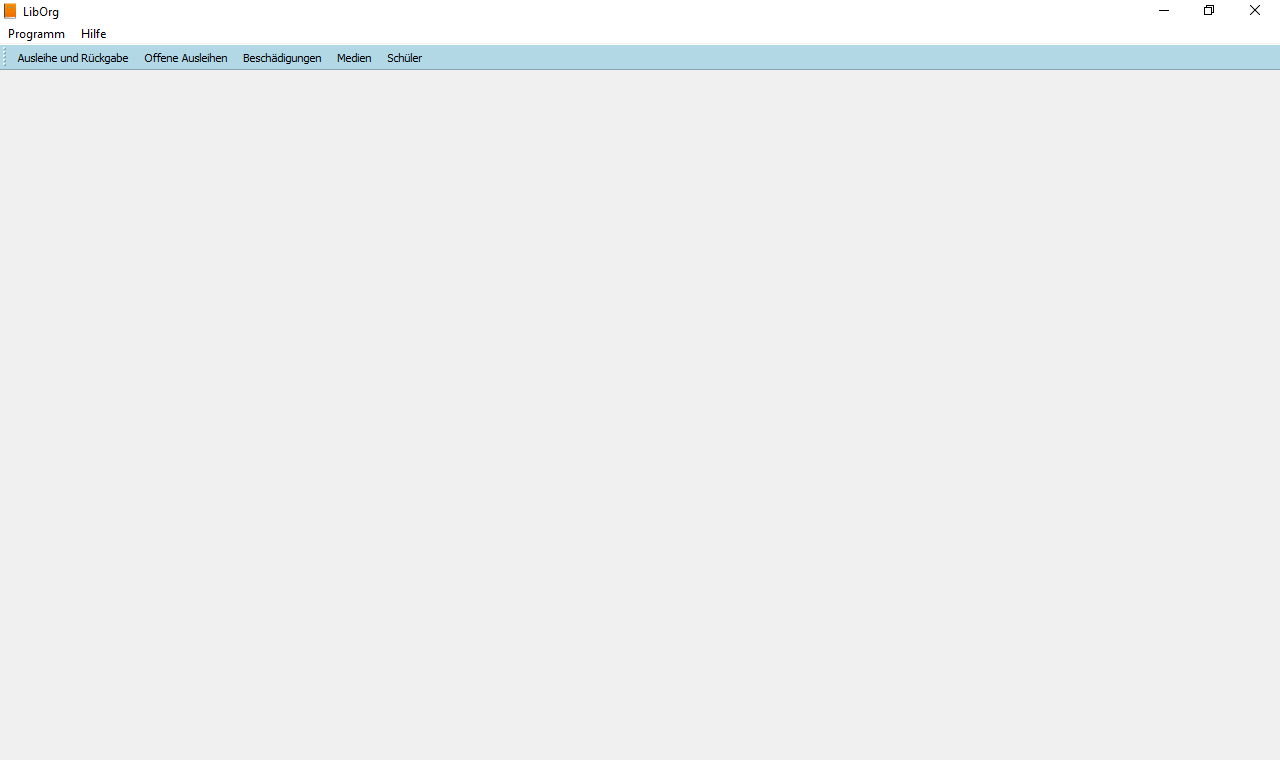
\includegraphics[width=0.70\textwidth]{figures/MainWindow.png}
	\caption{Hauptfenster}
	\label{fig:MainWindow}
\end{figure}

		\newpage
		\subsection{Installer (DH)}
\label{INSTALLER_HOWTO}
Um die Anwendung zum Kunden zu transferieren wird ein Installer-Projekt angelegt. Vor der Einrichtung des Installer-Projektes wird erläutert, welche Aufgaben ein Installer hat.\bigskip \\
Programme benötigen oft nicht nur die exe-Datei sondern auch andere Daten. Mit Hilfe eines Installers werden diese Dateien an den richtigen Ort kopiert. Wichtige Orte für ein Programm sind unter anderem: C:\textbackslash Programme bzw. C:\textbackslash Programme (x86) für statische Dateien (beispielsweise die exe-Datei und dlls), C:\textbackslash ProgramData für Dateien, die von mehreren Programmen benutzt werden, C:\textbackslash Benutzer für benutzerspezifische Dateien (z. B. Einstellungen) und C:\textbackslash Users\textbackslash Public\textbackslash Desktop für Verknüpfungen zur Anwendung \cite[vgl.][]{Installer_1}. Neben dem Kopieren der Dateien erlaubt es ein Installer zudem verschiedene Komponenten der Software auszuwählen. Des Weiteren können verschiedene Abhängigkeiten (z. B. Speicherplatz) überprüft werden \cite[vgl.][]{Installer_2}.\bigskip \\
Nachdem einige wichtige Aufgaben von Installer genannt worden sind, wird die Einrichtung des Installers unter Verwendung des Qt Installer-Frameworks beschrieben. Das Installer-Framework unterstützt die Auswahl eines Zielverzeichnisses für die Installation, die Auswahl von Komponenten und die Lizenzannahme \cite[vgl.][]{InstallerFramework1}. Die Lizenzdatei ist über die Online-Site app.legaltemplates.net erstellt worden.\\
Das Installer-Projekt muss manuell angelegt werden, hierzu muss folgende Struktur angelegt werden \cite[vgl][]{InstallerFramework2}:
\begin{itemize}
	\item Projektordner
	\begin{itemize}
		\item config
		\item packages
	\end{itemize}
\end{itemize}
In den config-Ordner werden eine config.xml-Datei und die Icon-Files (einmal als .ico für die Exe und einmal als .png für die Anwendung intern) eingefügt. In der config-Datei wird das Icon eingestellt, sowie der Autor und die Version des Installers eingetragen. Im packages-Ordner werden alle Komponenten, die installierbar sind, abgelegt. Dazu wird ein Ordner für jede Komponente angelegt, welcher die Unterordner data (darin sind die Dateien enthalten, die kopiert werden müssen) und meta enthält. Die Lizenzdatei und eine package.xml-Datei sind in diesem meta-Ordner enthalten. In der package.xml wird der Komponente ein Name und eine Beschreibung zugewiesen. Ebenfalls wird die Lizenzdatei hierin eingetragen und eingestellt, dass die Komponente installiert werden muss.\\
Nachdem die Struktur des Installers angelegt worden ist, muss die Datei deploy.bat ausgeführt werden. Dieses selbst erstellte Skript generiert einen Ornder bin und kopiert alle .dll, .exe und sonstige notwendigen Dateien aus dem Projekt in diesen Ordner. Anschließen wird der bin-Ordner gezippt und in das data-Verzeichnis der Komponente verschoben. Abschließend wird mit dem Skript createInstaller.bat der Installer erzeugt. 
\newpage
		\subsection{Dll's erzeugen und einbinden (FA)}
\label{DLLs_HOWTO}
Nachfolgend eine kurze Erklärung, wie man 'Dynamic Link Libraries' (kurz dll's) in Qt mithilfe des QtCreators und Visual Studio erzeugt und diese dann wiederum in ein beliebiges Programm einbindet. Als weitere Anleitungen bieten sich \cite{Dll_1} und \cite{Dll_2} an, welche eine Beschreibung für den QtCreator bieten und Teile von \cite{Dll_3}, die einige Einstiegsinformationen für Visual Studio enthalten. Am besten eignet sich jedoch die Video-Tutorials unter \cite{Dll_4} und \cite{Dll_5}, welche detaillierte Erklärungen liefern..

\subsubsection{Qt-Creator}
Zunächst muss ein neues Projekt für die dll erstellt werden. Hier muss als Vorlage 'C++-Bibliothek' gewählt werden, welche die nötigen Eigenschaften einer dll innerhalb des Projektes automatisch setzt (siehe Abbildung \ref{fig:proj}). \newline
\begin{figure}[H]
	\centering
	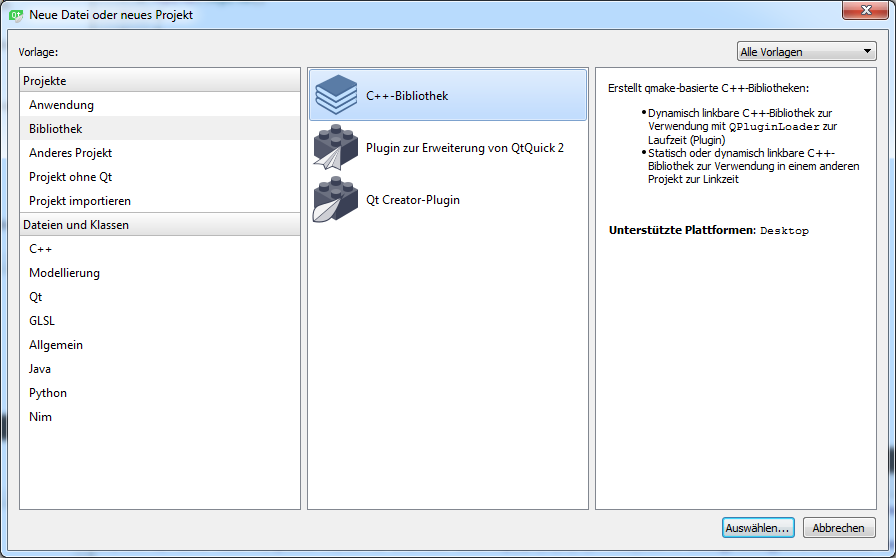
\includegraphics[width=0.90\textwidth]{figures/qtProjekt.png}
	\caption{Auswahl des Projekttyps}
	\label{fig:proj}
\end{figure}
Daraufhin ist es wichtig, die markierte Option 'dynamisch gebundene Bibliothek' auszuwählen (siehe Abbildung \ref{fig:bib}). Hier könnte man auch eine statische Bibliothek erzeugen, dies interessiert allerdings nicht.
\begin{figure}[H]
	\centering
	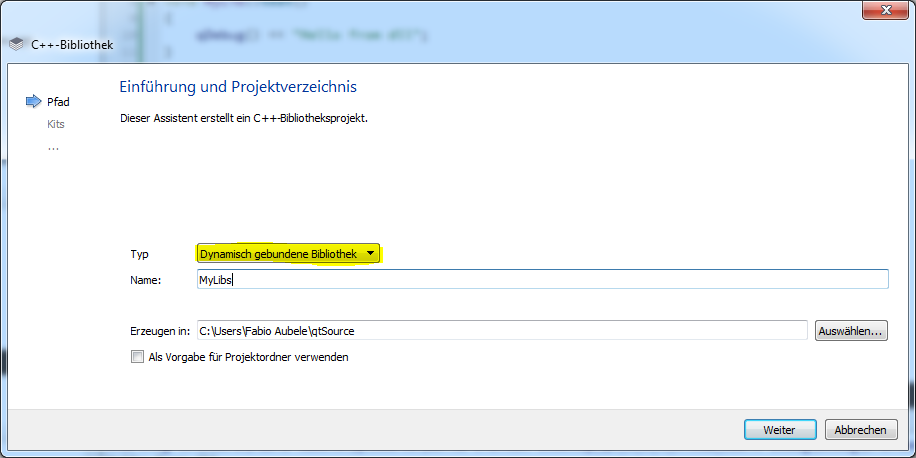
\includegraphics[width=0.90\textwidth]{figures/qtAuswahl.png}
	\caption{Auswahl des Bibliothekstyps}
	\label{fig:bib}
\end{figure}
Bei der Wahl des Compilers ist es wichtig KEINEN der Visual Studio Compiler (abgekürzt durch MSVC) auszuwählen, sondern MinGW (siehe Abbildung \ref{fig:comp}). Dies hat den Grund, dass Visual Studio eine etwas andere Form von DLLs erstellt, welche innerhalb des QtCreators beim Einbinden Fehler aufwerfen, da die DLL nicht lesbar ist.
\begin{figure}[H]
	\centering
	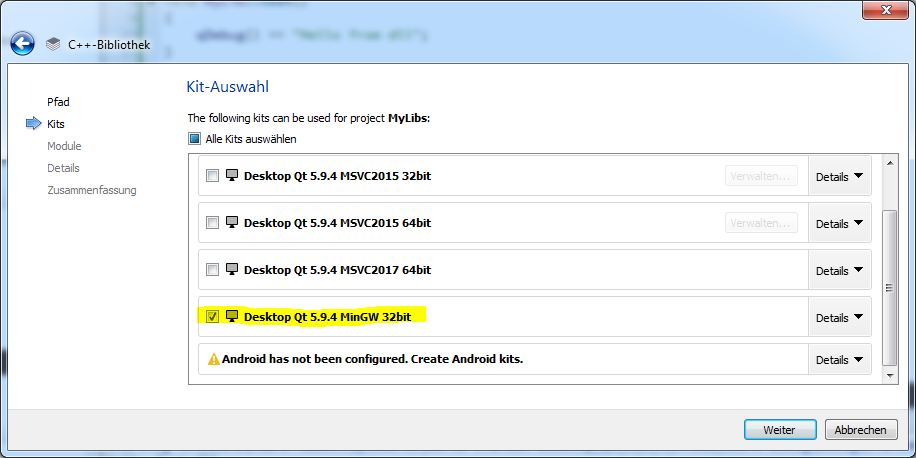
\includegraphics[width=0.90\textwidth]{figures/qtCompiler.png}
	\caption{Auswahl des Compilers}
	\label{fig:comp}
\end{figure}
Die restlichen Einstellung können beliebig abgeschlossen werden.\newline
Daraufhin kann das Projekt frei wählbar um weitere Dateien, Funktionen oder Klassen ergänzt werden. Wichtig ist, dass jede Header-Datei den globalen Header inkludiert (Im Beispiel: 'mylib\_global.h', siehe Abbildung \ref{fig:head}). Dahingegen muss jede Klasse in der Header-Datei das festgelegte Präfix am Anfang der Deklaration stehen haben (Im Beispiel: 'MYLIBSHARED\_EXPORT', siehe Abbildung \ref{fig:head}), dies gilt auch für Funktionen außerhalb von Klassen. \newline
Der globale Header wird automatisch bei der Erstellung des Projektes generiert. Dieser definiert den eben erwähnten Präfix, welcher sicherstellt, dass es sich um eine DLL handelt.
\begin{figure}[H]
	\centering
	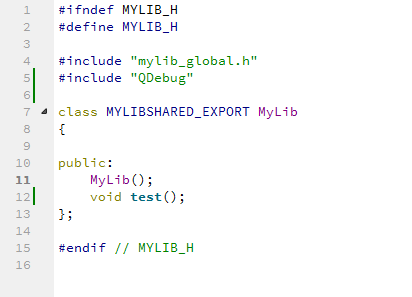
\includegraphics[width=0.40\textwidth]{figures/qtAufbau.png}
	\caption{Aufbau einer Header-Datei}
	\label{fig:head}
\end{figure}
Das Projekt, welches die DLL einbindet, kann ein zum Beispiel beliebiges GUI-Projekt sein, sollte aber auch nicht mit einem Visual Studio Compiler erstellt worden sein. In diesem müssen die Header-Dateien in das neue Projekt hinzugefügt werden. Dies sollte man in einem extra 'Include-Ordner' (zum Beispiel 'include' genannt) machen, damit die Übersicht über die Dateien leichter beibehalten werden kann. Ebenfalls muss die erzeugte DLL-Datei mit der dazugehörigen '*.a-Datei' in das neue Projekt hinzugefügt werden. Dafür sollte ebenfalls ein zusätzlicher Ordner erstellt werden (zum Beispiel 'lib' genannt). In diesen Ordner die '*.dll-Datei' hinzufügen. Daraufhin muss die Bibliothek der Applikation bekannt gemacht werden. Dies geschieht mithilfe des Dialogs unter Abbildung \ref{fig:Pro}.
\begin{figure}[H]
	\centering
	\includegraphics[width=0.60\textwidth]{figures/qtPro.png}
	\caption{Bibliothek hinzufügen}
	\label{fig:Pro}
\end{figure}
Hier wählt man 'externe Bibliothek', daraufhin öffnet man unter 'Bibliotheksdatei' die '*.a-Datei', welche man in den erstellten 'lib-Ordner' gezogen hat. In Abbildung \ref{fig:bibdatei} sieht man beispielhafte Einstellungen, welche bis auf die Pfade übernommen werden können. 
\begin{figure}[H]
	\centering
	\includegraphics[width=0.40\textwidth]{figures/qtBibdatei.png}
	\caption{Einstellungen für die Bibliothek angeben}
	\label{fig:bibdatei}
\end{figure}
Dies bereitet das System auf die dll vor und legt Einträge in der 'pro-Datei' an. Debug und Release Versionen werden hier nicht berücksichtigt. \newline
Nun muss nur noch der gewünschte Header inkludiert und die Funktion oder Klasse aufgerufen werden (siehe Abbildung \ref{fig:Final}).
\begin{figure}[H]
	\centering
	\includegraphics[width=0.30\textwidth]{figures/qtFinal.png}
	\caption{Aufruf der dll}
	\label{fig:Final}
\end{figure}

\subsubsection{Visual Studio}
Das Erzeugen einer dll läuft in den selben Schritten ab wie oben beschrieben. Einzig die Oberfläche der Dialoge ist etwas anders und die Voreinstellung des Projektes lautet 'Qt Class Library' und nicht 'C++-Bibliothek'. \newline
Auch das Editieren des dll-Projektes läuft exakt gleich ab und die vorgefertigten Dateien sind gleich aufgebaut. Jetzt zu den Unterschieden. Als Ausgabe bekommt man hier nicht nur eine '*.dll-Datei', sondern auch eine '*.lib-Datei'. Beide Dateien sind wichtig beim Einbinden der dll. \newline
\newline
Zum Einbinden kann wieder eine beliebige Gui-Applikation dienen. Anfänglich müssen im Verzeichnis der Applikation wieder zwei neue Ordner erstellt werden. Einmal ein 'include-Ordner', hier werden wieder die gewünschten Header-Dateien hinzugefügt und zusätzlich auch der global-Header, wie auch oben beschrieben. Des Weiteren wird auch ein 'lib-Ordner erstellt, hier wird jedoch die '*.lib-Datei' und nicht wie oben die '*.dll-Datei' hinzugefügt. In Abbildung \ref{fig:ordner} sieht man die Ordnerstruktur, markiert sind hier die neuen Ordner.
\begin{figure}[H]
 	\centering
 	\includegraphics[width=0.80\textwidth]{figures/vsOrdner.png}
 	\caption{Ordnerstruktur}
 	\label{fig:ordner}
\end{figure}
Nun müssen einige Projekteinstellungen geändert werden, damit Visual Studio die neuen Verzeichnisse und Dateien erkennt und benutzt. Zunächst muss der Include-Ordner bekannt gemacht werden, dies ist unter Projekt -> Projekteigenschaften -> C/C++ -> Allgemein -> Zusätzliche Includeverzeichnisse zu tun. In Abbildung \ref{fig:inc} sieht man den hinzugefügten Eintrag:
\begin{figure}[H]
	\centering
	\includegraphics[width=0.40\textwidth]{figures/vsInclude.png}
	\caption{Eintrag des Includeverzeichnisses}
	\label{fig:inc}
\end{figure}
Daraufhin ist der 'lib-Ordner' preiszugeben. Dies geschieht unter Projekt -> Projekteigenschaften -> Linker -> Zusätzliche Bibliotheksverzeichnisse. In Abbildung \ref{fig:bibV} sieht man den Eintrag:
\begin{figure}[H]
	\centering
	\includegraphics[width=0.40\textwidth]{figures/vsBib.png}
	\caption{Eintrag des Bibliotheksverzeichnisses}
	\label{fig:bibV}
\end{figure}
Schlussendlich muss Visual Studio noch der Name der Datei innerhalb des 'lib-Ordners' mitgeteilt werden. Dies ist möglich unter Projekt -> Projekteigenschaften -> Linker -> Eingabe. In Abbildung \ref{fig:bibV2} sieht man den Eintrag:
\begin{figure}[H]
	\centering
	\includegraphics[width=0.40\textwidth]{figures/vsBib2.png}
	\caption{Eintrag der Bibliothek}
	\label{fig:bibV2}
\end{figure}
Zum Schluss muss in das Build-Verzeichnis, in welchem auch die '*.exe-Datei' liegt, die '*.dll-Datei' hinzufügt werden (meist unter x64 -> Debug oder x86 -> Debug). Nun kann man die gewünschte Header-Datei inkludieren und je nach Belieben Funktionen und Klassen aufrufen (siehe Abbildung \ref{fig:Final2}).
\begin{figure}[H]
	\centering
	\includegraphics[width=0.40\textwidth]{figures/vsFinal.png}
	\caption{Aufruf der dll}
	\label{fig:Final2}
\end{figure}
\newpage
		\subsection{Updatemechanismus - Funktionsweise (DH)}
Um eine Update-Funktion zu implementieren, wird ein eigenes Programm (eine eigene Exe) erstellt. Zu beachten ist, dass dieses Programm selber nicht aktualisiert werden kann. Der Grund hierfür liegt in der Aufgabe des eigenständigen Programms: Es überprüft auf einem Server, ob neue oder geänderte Dateien vorliegen, lädt diese herunter und installiert sie. Die heruntergeladenen Dateien können DLLs, Konfiguration oder ein Programm (Exe) sein. Das Programm, welches diese Dateien herunterlädt, kann vom Hauptprogramm aus ausgeführt werden. Dann muss das Hauptprogramm aber nach Ausführung des Update-Programms beendet und nach dem Update-Prozess wieder neu gestartet werden \cite[vgl.][]{HOW_Update}.\\
Was geschieht bei der Installation? Kurz gesagt, werden alle notwendigen Dateien an die richtige Stelle kopiert, so dass sie vom Hauptprogramm aus gefunden werden. Außerdem können Umgebungsvariablen und Registry-Einträge geschrieben sowie Verknüpfungen erstellt werden. Es geschehen jedoch noch weitere Vorgänge während einer Installtion, der Installationsprozess wird im Kapitel zur Erstellung des Installers genauer erläutert.\\
Die Hauptanwendung kann vorerst ohne Rücksicht auf den Update-Prozess entwickelt werden, wodurch die Funktion des Updates von der Priorität nach ganz hinten rückt. Zu beachten ist lediglich, dass sich die Datenbank, also die Tabellendefinitionen, nicht ändern dürfen. Eine Aktualisierung der Datenbank ist sehr aufwendig und fehleranfällig. Aus diesem Grund wird strikt darauf geachtet, dass die Datenbank nicht mehr verändert werden muss.
\newpage
		\subsection{Usabilityaspekte (FA)}
\label{USABILITY_ASPEKTE}
In folgendem sollen einige wichtige Informationen zur Usability bekannt gegeben werden. Dabei wird zuerst ein Überblick aufgezeigt, welcher erklärt, was für Aspekte zu dem Thema Usability gehören und für dieses Projekt relevant sind. Daraufhin werden Normen präsentiert, welche die Themen Gebrauchstauglichkeit und Dialoggestaltung detailliert behandeln. Auf die dort geschilderten Aspekte und Grundsätze ist innerhalb der Projektarbeit Rücksicht zu nehmen.

\subsubsection{Usability-Kennzahlen}
Um Usability zu definieren, ist es wichtig aktuelle Qualitätskriterien für Software zu kennen. Eines davon ist der Human Factor, dessen wichtigstes Kriterium die Benutzerfreundlichkeit ist. Unter Benutzerfreundlichkeit wird dabei verstanden, wie die Funktionalitäten der Anwendung dem Benutzer präsentiert werden. Die Herausforderung dabei ist, die Bedürfnisse der Benutzer zu verstehen und diese in die Software einfließen zu lassen \cite{usability}.\newline 
Eine verbesserte Benutzerfreundlichkeit ist dabei ausschlaggebend für gute Software. Sie wirkt sich auf die Effizienz und Produktivität, die Sicherheit, den Bedarf an Schulungen und die Akzeptanz der Software aus \cite{usability}.
Gemäß \cite{usability} wird die Benutzerfreundlichkeit mit nachfolgenden Kriterien bewertet:
\begin{itemize}
	\item Dauer die zum Erlernen der Software notwendig ist
	\item Vorhersagbarkeit
	\item Synthetisierbarkeit: Möglichkeit der Beurteilung der letzten Operation
	\item Vertrautheit
	\item Generalisierbarbeit
	\item Konsistenz
	\item Dauer für die Erfüllung einer Aufgabe
	\item Fehlerrate von Benutzern
	\item Persistenz der Schnittstellenkonzepte
	\item Subjektive Zufriedenheit
	\item Flexibilität: Dialog-Initiative, Multithreading, Substituierbarkeit, Anpassbarkeit
	\item Robustheit: Beobachtbarkeit, Wiederherstellbarkeit, Reaktionsfähigkeit
\end{itemize}

\subsubsection{Norm für Gebrauchstauglichkeit - DIN EN ISO 9241-11}
Nachfolgender Text ist ein Auszug von \cite{DIN1} und legt eine Reihe von Aktivitäten fest, die zur Erreichung der Gebrauchstauglichkeit angewendet werden können: \newline
\newline
a) Verstehen und Beschreiben des Nutzungskontextes:\newline
Diese Aktivität legt fest, was der/die maßgebende(n) Nutzungskontext(e) ist/sind, so dass die Informationen in der Anforderungsspezifikation verwendet werden können, sowie bei der Überlegung, welche Gestaltungslösungen in diesen Kontexten nutzbar sind.\newline
Gebrauchstauglichkeit kann für verschiedene Anwendungsbereiche eines Nutzungskontextes betrachtet werden, zum Beispiel: Alle potenziell maßgebenden Nutzungskontexte, Ausgewählte Nutzungskontexte, Ein Einzelfall des Nutzungskontextes, Nutzungskontext für eine Einzelperson.\newline
\newline
b) Spezifizierung der Benutzeranforderungen:\newline
Die Identifizierung von Benutzerbedürfnissen kann die Grundlage für die Spezifizierung von Benutzeranforderungen bilden. Die Spezifizierung der Benutzeranforderungen umfasst die Identifizierung der maßgeblichen Anforderungen an die Gebrauchstauglichkeit (d. h. Kriterien für Effektivität, Effizienz und Zufriedenstellung in bestimmten Nutzungskontexten). \newline
Beispiel: Für eine E-Commerce-Website könnten die wichtigsten Ziele Effektivität (Genauigkeit und Vollständigkeit) und Zufriedenstellung (positive Einstellungen und Emotionen einschließlich Vertrauen und Spaß) für einen gelegentlichen Benutzer sein.\newline
\newline
c) Gestaltungslösungen entwerfen:\newline
Diese Aktivität beinhaltet u. a. die Anwendung des Nutzungskontextes und der Benutzeranforderungen in Verbindung mit ergonomischen Kenntnissen, um zum Entwurf einer gebrauchstauglichen Gestaltungslösung beizutragen.\newline
\newline
d) Evaluierung der Gestaltung:\newline
Diese Aktivität evaluiert mögliche Gestaltungslösungen und/oder bereits vorhandene Produkte oder Dienstleistungen und bietet Rückmeldungen zu ihrer Gebrauchstauglichkeit.\newline
Die spezifischen Ziele, für die die Gebrauchstauglichkeit des interessierenden Objekts betrachtet wird, können zur Identifizierung der jeweiligen Bedeutung von Effektivität, Effizienz und Zufriedenstellung oder ihrer Elemente sowie zu einem oder mehreren Maßen für jedes dieser Merkmale führen. Es ist wichtig, dass diese Maße sich glaubwürdig und verlässlich auf die identifizierten Ziele beziehen.\newline
Die Evaluierung kann sich auf das/die Endergebnis(se) oder auf die Ergebnisse von Interaktionen unter Nutzung des interessierenden Objektes konzentrieren.\newline
Gestaltungslösungen oder Systeme können evaluiert werden, um festzustellen, ob sie die Benutzer-anforderungen innerhalb eines bestimmten Nutzungskontextes erfüllen, und/oder um Probleme im Zusammenhang mit der Gebrauchstauglichkeit innerhalb eines bestimmten Nutzungskontextes zu erkennen.

\subsubsection{Norm für Dialoggestaltung - DIN EN ISO 9241-110}
Nachfolgender Text stammt von \cite{DIN2} und stellt Grundsätze vor, welche bei der Dialoggestaltung berücksichtigt werden sollten: \newline
\\
Die folgenden sieben Grundsätze sind für die Gestaltung und Bewertung eines Dialoges wichtig:\newline
\newline
a) Aufgabenangemessenheit:\newline
Ein interaktives System ist aufgaben-angemessen, wenn es den Benutzer unterstützt, seine Arbeitsaufgabe zu
erledigen, d. h., wenn Funktionalität und Dialog auf den charakteristischen Eigenschaften der Arbeitsaufgabe
basieren, anstatt auf der zur Aufgabenerledigung eingesetzten Technologie. Darunter fällt:
\begin{itemize}
	\item Der Dialog sollte dem Benutzer solche Informationen anzeigen, die im Zusammenhang mit der
	erfolgreichen Erledigung der Arbeitsaufgabe stehen.
	\item Der Dialog sollte dem Benutzer keine Informationen anzeigen, die nicht für die erfolgreiche Erledigung relevanter Arbeitsaufgaben benötigt werden.
	\item Die Form der Eingabe und Ausgabe sollte der Arbeitsaufgabe angepasst sein.
	\item Wenn für eine Arbeitsaufgabe ganz bestimmte Eingabewerte typisch sind, sollten diese Werte dem
	Benutzer automatisch als voreingestellte Werte verfügbar sein.
	\item Die vom interaktiven System verlangten Dialogschritte sollten zum Arbeitsablauf passen, d. h.,
	notwendige Dialogschritte sollten enthalten sein und unnötige Dialogschritte sollten vermieden werden.
	\item Wenn bei einer Arbeitsaufgabe Quelldokumente verwendet werden, sollte die Benutzungsschnittstelle
	kompatibel zu den charakteristischen Eigenschaften der Quelldokumente sein.
	\item Die Eingabe- und Ausgabemedien des interaktiven Systems sollten aufgabenangemessen sein.
\end{itemize}
b) Selbstbeschreibungsfähigkeit:\newline
Ein Dialog ist in dem Maße selbstbeschreibungsfähig, in dem für den Benutzer zu jeder Zeit offensichtlich ist,
in welchem Dialog, an welcher Stelle im Dialog er sich befindet, welche Handlungen unternommen werden
können und wie diese ausgeführt werden können. Hierfür gilt:
\begin{itemize}
	\item Die bei jedem Dialogschritt angezeigten Informationen sollten den Benutzer leiten, den Dialog
	erfolgreich abzuschließen.
	\item Während der Interaktion mit dem System sollte die Notwendigkeit, Benutzer-Handbücher und andere
	externe Informationen heranzuziehen, minimiert sein.
	\item Der Benutzer sollte über Änderungen des Zustandes des interaktiven Systems informiert werden, also wann Eingaben erwartet werden und durch Bereitstellung eines Überblickes über die nächsten Dialogschritte.
	\item Wenn eine Eingabe verlangt wird, sollte das interaktive System dem Benutzer Informationen über die
	erwartete Eingabe bereitstellen.
	\item Dialoge sollten so gestaltet sein, dass die Interaktion für den Benutzer offensichtlich ist.
	\item Das interaktive System sollte dem Benutzer Informationen über die erforderlichen Formate und
	Einheiten bereitstellen.
\end{itemize}
c) Erwartungskonformität:\newline
Ein Dialog ist erwartungskonform, wenn er den aus dem Nutzungskontext heraus vorhersehbaren Benutzerbelangen
sowie allgemein anerkannten Konventionen entspricht.
\begin{itemize}
	\item Das interaktive System sollte das Vokabular verwenden, das dem Benutzer bei der Ausführung der
	Arbeitsaufgabe vertraut ist oder von ihm auf Grund seiner Kenntnisse und Erfahrungen verwendet wird.
	\item Auf Handlungen des Benutzers sollte eine unmittelbare und passende Rückmeldung folgen, soweit
	dies den Erwartungen des Benutzers entspricht.
	\item Kann vorhergesehen werden, dass erhebliche Abweichungen von der vom Benutzer erwarteten
	Antwortzeit entstehen, sollte der Benutzer hiervon unterrichtet werden.
	\item Informationen sollten so strukturiert und organisiert sein, wie es vom Benutzer als natürlich
	empfunden wird.
	\item Formate sollten geeigneten kulturellen und sprachlichen Konventionen entsprechen.
	\item Art und Länge von Rückmeldungen oder Erläuterungen sollten den Benutzerbelangen entsprechen.
	\item Dialogverhalten und Informationsdarstellung eines interaktiven Systems sollten innerhalb von
	Arbeitsaufgaben und über ähnliche Arbeitsaufgaben hinweg konsistent sein.
	\item Wenn eine bestimmte Eingabeposition auf der Grundlage von Benutzererwartungen vorhersehbar ist,
	dann sollte diese Position für die Eingaben voreingestellt sein.
	\item Rückmeldungen oder Mitteilungen, die dem Benutzer angezeigt werden, sollten in einer objektiven
	und konstruktiven Art formuliert sein.
\end{itemize}
d) Lernförderlichkeit:\newline
Ein Dialog ist lernförderlich, wenn er den Benutzer beim Erlernen der Nutzung des interaktiven Systems
unterstützt und anleitet.
\begin{itemize}
	\item Regeln und zugrunde liegende Konzepte, die für das Erlernen nützlich sind, sollten dem Benutzer
	zugänglich gemacht werden.
	\item Wenn ein Dialog selten gebraucht wird oder charakteristische Eigenschaften des Benutzers es
	erfordern, den Dialog erneut zu erlernen, dann sollte geeignete Unterstützung dafür bereitgestellt werden.
	\item Geeignete Unterstützung sollte bereitgestellt werden, damit der Benutzer mit dem Dialog vertraut wird.
	\item Rückmeldung und Erläuterungen sollten den Benutzer unterstützen, ein konzeptionelles Verständnis
	vom interaktiven System zu bilden.
	\item Der Dialog sollte ausreichende Rückmeldung über Zwischen- und Endergebnisse von Handlungen
	bereitstellen, damit die Benutzer von erfolgreich ausgeführten Handlungen lernen.
	\item Falls es zu den Arbeitsaufgaben und den Lernzielen passt, sollte das interaktive System dem
	Benutzer erlauben, Dialogschritte ohne nachteilige Auswirkungen neu auszuprobieren.
	\item Das interaktive System sollte es dem Benutzer ermöglichen, die Arbeitsaufgabe mit minimalem
	Lernaufwand auszuführen, indem es den Dialog mit minimaler Eingabe von Informationen ermöglicht, jedoch
	zusätzliche Information auf Anforderung zur Verfügung stellt.
\end{itemize}
e) Steuerbarkeit:\newline
Ein Dialog ist steuerbar, wenn der Benutzer in der Lage ist, den Dialogablauf zu starten sowie seine Richtung
und Geschwindigkeit zu beeinflussen, bis das Ziel erreicht ist.
\begin{itemize}
	\item Die Geschwindigkeit der Interaktion sollte nicht durch das interaktive System vorgegeben werden. Sie
	sollte vom Benutzer steuerbar sein, und zwar unter Berücksichtigung der Benutzerbelange und der
	charakteristischen Eigenschaften des Benutzers.
	\item Der Benutzer sollte die Steuerung darüber haben, wie der Dialog fortgesetzt wird.
	\item Ist der Dialog unterbrochen worden, sollte der Benutzer die Möglichkeit haben, den
	Wiederaufnahmepunkt der Fortsetzung des Dialoges zu bestimmen, falls es die Arbeitsaufgabe erlaubt.
	\item Wenigstens der letzte Dialogschritt sollte zurückgenommen werden können, soweit Handlungsschritte
	reversibel sind und falls es der Nutzungskontext erfordert.
	\item Wenn die Datenmenge, die für eine Arbeitsaufgabe von Bedeutung ist, groß ist, dann sollte der
	Benutzer die Möglichkeit haben, die Anzeige der dargestellten Datenmenge zu steuern.
	\item Der Benutzer sollte dort, wo es geeignet ist, die Möglichkeit haben, jedes verfügbare 	Eingabe-/Ausgabemittel benutzen zu können.
	\item Wenn es für die Arbeitsaufgabe zweckmäßig ist, sollte der Benutzer voreingestellte Werte ändern
	können.
	\item Wenn Daten verändert wurden, sollten die Originaldaten für den Benutzer verfügbar bleiben, wenn
	dies für die Arbeitsaufgabe erforderlich ist.
\end{itemize}
f) Fehlertoleranz:\newline
Ein Dialog ist fehlertolerant, wenn das beabsichtigte Arbeitsergebnis trotz erkennbar fehlerhafter Eingaben
entweder mit keinem oder mit minimalem Korrekturaufwand seitens des Benutzers erreicht werden kann.
Fehlertoleranz wird erreicht mit Fehlererkennung und -vermeidung (Schadensbegrenzung), Fehlerkorrektur oder Fehlermanagement, um mit Fehlern umzugehen, die sich ereignen.
\begin{itemize}
	\item Das interaktive System sollte den Benutzer dabei unterstützen, Eingabefehler zu entdecken und zu
	vermeiden.
	\item Das interaktive System sollte verhindern, dass irgendeine Benutzer-Handlung zu undefinierten
	Systemzuständen oder zu Systemabbrüchen führen kann.
	\item Wenn sich ein Fehler ereignet, sollte dem Benutzer eine Erläuterung zur Verfügung gestellt werden,
	um die Beseitigung des Fehlers zu erleichtern.
	\item Aktive Unterstützung zur Fehlerbeseitigung sollte dort, wo typischerweise Fehler auftreten, zur
	Verfügung stehen.
	\item Wenn das interaktive System Fehler automatisch korrigieren kann, sollte es den Benutzer über die
	Ausführung der Korrektur informieren und ihm Gelegenheit geben, zu korrigieren.
	\item Der Benutzer sollte die Möglichkeit haben, die Fehlerkorrektur zurückzustellen oder den Fehler
	unkorrigiert zu lassen, es sei denn, eine Korrektur ist erforderlich, um den Dialog fortsetzen zu können.
	\item Wenn möglich, sollten dem Benutzer auf Anfrage zusätzliche Informationen zum Fehler und dessen
	Beseitigung zur Verfügung gestellt werden.
	\item Die Prüfung auf Gültigkeit und Korrektheit von Daten sollte stattfinden, bevor das interaktive System
	die Eingabe verarbeitet.
	\item Die zur Fehlerbehebung erforderlichen Schritte sollten minimiert sein.
	\item Falls sich aus einer Benutzerhandlung schwerwiegende Auswirkungen ergeben können, sollte das
	interaktive System Erläuterungen bereitstellen und Bestätigung anfordern, bevor die Handlung ausgeführt
	wird.
\end{itemize}
g) Individualisierbarkeit:\newline
Ein Dialog ist individualisierbar, wenn Benutzer die Mensch-System-Interaktion und die Darstellung von
Informationen ändern können, um diese an ihre individuellen Fähigkeiten und Bedürfnisse anzupassen.
\begin{itemize}
	\item Das interaktive System sollte dem Benutzer dort, wo unterschiedliche Benutzerbelange typischerweise
	vorkommen, Techniken zur Anpassung an die charakteristischen Eigenschaften von Benutzern
	bereitstellen.
	\item Das interaktive System sollte es dem Benutzer erlauben, zwischen verschiedenen Formen der
	Darstellung zu wählen, wenn es für die individuellen Bedürfnisse unterschiedlicher Benutzer zweckmäßig ist.
	\item Der Umfang von Erläuterungen (z. B. Details in Fehlermeldungen, Hilfeinformationen) sollte
	entsprechend dem individuellen Wissen des Benutzers veränderbar sein.
	\item Benutzer sollten, soweit zweckmäßig, die Möglichkeit haben, eigenes Vokabular einzubinden, um
	Objekte und Funktionen („Werkzeuge“) individuell zu benennen.
	\item Der Benutzer sollte, soweit zweckmäßig, die Geschwindigkeit von dynamischen Eingaben und
	Ausgaben einstellen können, um sie an seine individuellen Bedürfnisse anzupassen.
	\item Die Benutzer sollten, soweit zweckmäßig, die Möglichkeit haben, zwischen unterschiedlichen
	Dialogtechniken zu wählen.
	\item Der Benutzer sollte die Möglichkeit haben, das Niveau und die Methoden der Mensch-System-
	Interaktion so auszuwählen, dass sie am besten seinen Bedürfnissen entsprechen.
	\item Der Benutzer sollte die Möglichkeit haben, die Art zu wählen, in der Eingabe-/Ausgabe-Daten
	dargestellt werden (Format und Typ).
	\item Soweit zweckmäßig, sollte es den Benutzern möglich sein, Dialogelemente oder Funktionen
	hinzuzufügen oder neu zu ordnen, insbesondere, um individuelle Bedürfnisse bei der Ausführung von
	Arbeitsaufgaben zu unterstützen.
	\item Individuelle Einstellungen eines Dialoges sollten rückgängig gemacht werden können und es dem
	Benutzer erlauben, zu den ursprünglichen Einstellungen zurückzugehen.
\end{itemize}
\newpage

		\subsection{Konfiguration (DH)}
Damit Anwender diverse Einstellungen an der Software vornehmen und diese permanent speichern können, wird eine Klassenbibliothek für die Verwaltung von Konfigurationseinträgen erstellt. Zudem soll die Bibliothek in der Lage sein, anhand der vorhandenen Konfigurationseinträge eine automatische Oberfläche für die Änderung der Konfigurationseinträge zu generieren.

\subsubsection{Benötigte Typen}
Um die Form der Konfigurationsdatei zu bestimmen, wird zunächst betrachtet, welche Art von Einträgen sich in einer Konfiguration befinden können. Diese sind in Tabelle \ref{tab:Konfigurationstypen} aufgelistet. Außerdem wird jedem Typ ein Darstellungselement zugeordnet.
\begin{table}[htb]
	\centering
	\caption{Konfigurationstypen}
		\begin{tabular}{|c|c|c|}
			\hline
			Boolsche Werte (1: True, 0: False) & Checkbox & bool \\ \hline
			Text (ggf. mit Längenbeschränkung) & LineEdit & string\\ \hline
			Text mit Vorauswahl (ggf. mit Längenbeschränkung) & ComboBox & chosestring\\ \hline
			Text mit Vorauswahl und Eingabemöglichkeit & ComboBox & choseentrystring \\ \hline
			Ganzzahlen & SpinBox & int\\ \hline
			Gleitzahlen & DoubleSpinBox & double\\ \hline
			RGB-Farbe & LineEdit + Button & rgbcolor\\ \hline
			Blöcke & GroupBox & siehe unten\\ \hline
			Kommentare / Beschreibungen & Label & siehe unten \\ \hline
			Read-only Werte & Element nur lesend & \\ \hline
		\end{tabular}
	\label{tab:Konfigurationstypen}
\end{table}

\subsubsection{Format der Konfigurationsdateien}
Nachdem alle notwendigen Typen ermittelt wurden, wird die Struktur der Konfigurationseinträge bestimmt. Tabelle \ref{tab:Konfigurationsoptionen} enthält alle verwendbaren Zeichen und deren Bedeutung.
\begin{table}[htb]
	\centering
	\caption{Konfigurationsoptionen}
		\begin{tabular}{|c|c|}
			\hline
			$[$ $]$ & Blockname \\ \hline
			\# & Kommentar / Beschreibung \\ \hline
			$<$ $>$ & Auswahlmöglichkeiten \\ \hline
			; & Wertetrennung \\ \hline
			: & Typ \\ \hline
			$=$ & Wertzuweisung \\ \hline
			$($ $)$ & Bereichsangabe / Länge \\ \hline
			\{ \} & readonly \\ \hline
			\#! & Startkommentar \\ \hline
		\end{tabular}
	\label{tab:Konfigurationsoptionen}
\end{table}
Um die Syntax der Konfigurationsdateien zu beschreiben, wird nachfolgendes Beispiel verwendet, das alle Konfigurationsoptionen enthält.
\begin{verbatim}
#! Beispiel-Konfig example.config
# Erster Block
[Erster Block]
# Ganzzahliger Schlüssel mit Minimum und Maximum
Var1: int = 5
(1;5)

# Boolscher Schlüssel
Var2: bool = 1

# Text mit Länge 5
Var3: string = Hallo
(5)

# Text mit Vorauswahl
Var4: chosestring = H1
<H1; H2; H3>

# Text mit Vorauswahl und Eingabemöglichkeit
Var5: choseentrystring = H1
<H1; H2; H3>

# Gleitzahl read-only
{Var6: double = 6.3}
\end{verbatim}

\subsubsection{VariousValue}
VariousValue wird benutzt, um die QVariant-Klasse von Qt nachzubilden. Die Klasse kann damit mehrere verschiedene Datentypen beinhalten, ohne auf das QMetaSystem zugreifen zu müssen.\bigskip \\
\textbf{Header:} variousvalue.h\bigskip \\
\textbf{Library:} baseqt.dll\bigskip \\
\textbf{enum}\\
type: Int, Double, Text, SelectText, SelectEntryText, Bool, RGB\_Color\bigskip \\
\textbf{Öffentliche Methoden}\\
\small{VariousValue(type valuetype, QString value)}\\
Erzeugt ein VariousValue-Objekt.\bigskip \\
\small{int asInt()}\\
Liefert den Wert des VariousValue falls möglich als integer zurück.\bigskip \\
\small{double asDouble()}\\
Liefert den Wert des VariousValue falls möglich als double zurück.\bigskip \\
\small{bool asBool()}\\
Liefert den Wert des VariousValue falls möglich als bool zurück.\bigskip \\
\small{QString asText() noexcept}\\
Liefert den Wert des VariousValue falls möglich als QString zurück.\bigskip \\
\small{QColor asColor()}\\
Liefert den Wert des VariousValue falls möglich als QColor zurück.\bigskip \\
\small{bool setValue(QString newvalue) noexcept}\\
Aktualisiert den Wert des VariousValue-Objektes, liefert true zurück, wenn dies erfolgreich war.\bigskip \\
\small{type getType()}\\
Liefert den Typ des VariousValue-Objektes.

\subsubsection{ConfigObserver}
Abstrakte Klasse, die die Config-Objekte beobachten kann.\bigskip \\
\textbf{Header:} config.h\bigskip \\
\textbf{Library:} baseqt.dll\bigskip \\
\textbf{enum}\\
Action: ADDED, REMOVED, MODIFIED\bigskip \\
\textbf{Öffentliche Methoden}\\
\small{virtual void cfgblockchanged(QString blockname, Action action) noexcept = 0}\\
Wird von der Config-Klasse aufgerufen, wenn sich ein Block der Konfiguration geändert hat.\bigskip \\
\small{virtual void cfgkeyofblockchanged(QString blockname, QString keyname, Action action) noexcept = 0}\\
Wird von der Config-Klasse aufgerufen, wenn sich ein Schlüssel eines Blocks der Konfiguration geändert hat.

\subsubsection{Config}
Die Klasse Config besteht aus Blöcken, welche wiederum aus den Konfigurationsschlüsseln bestehen.\bigskip \\
\textbf{Header:} config.h\bigskip \\
\textbf{Library:} baseqt.dll\bigskip \\
\textbf{Öffentliche Methoden}\\
\small{Config(QString cfgName, QString path)}\\
Erzeugt ein Config-Objekt ohne Blöcke und Schlüssel.\bigskip \\
\small{\~{}Config()}\\
Zerstört das Objekt inklusive aller Blöcke und Schlüssel.\bigskip \\
\small{QString getConfigName() noexcept}\\
Liefert den Namen des Config-Objektes.\bigskip \\
\small{QString getConfigComment}\\
Liefert den Kommentar der Konfiguration.\bigskip \\
\small{bool isModified() noexcept}\\
Liefert, ob das Config-Objekt verändert wurde.\bigskip \\
\small{void attach(ConfigObserver* observer) noexcept}\\
Hängt einen neuen Observer an die Konfiguration an.\bigskip \\
\small{void detach(ConfigObserver* observer) noexcept}\\
Entfernt den übergebenen Oberserver von der Konfiguration. \bigskip \\
\small{VariousValue getValueForKeyInBlock(QString blockname, QString keyname, VariousValue defaultvalue) noexcept}\\
Liefert den Wert des Schlüssels in dem spezifizierten Block der Konfiguration zurück. Ist kein gültiger Schlüssel vorhanden, wird der defaultvalue zurückgegeben.\bigskip \\
\small{bool addBlock(QString blockname, QString blockcomment) noexcept}\\
Fügt einen neuen Block an die Konfiguration an.\bigskip \\
\small{void removeBlock (QString blockname) noexcept}\\
Entfernt einen Block aus der Konfiguration.\bigskip \\
\small{QString getCommentOfBlock(QString blockname)}\\
Liefert den Kommentar eines Blocks einer Konfiguration. \bigskip \\
\small{QList<QString> getAllBlocks() noexcept}\\
Liefert eine Liste mit allen vorhandenen Blöcken der Konfiguration.\bigskip \\
\small{QList<QString> getAllKeysOfBlock(QString blockname)}\\
Liefert alle Schlüssel eines Blocks der Konfiguration.\bigskip\\
\small{bool addKeyToBlock(QString blockname, QString keyname, QString keycomment, VariousValue value, bool isReadOnly = false) noexcept}\\
Fügt einen Schlüssel an den Block einer Konfiguration an.\bigskip \\
\small{bool removeKeyFromBlock(QString blockname, QString keyname) noexcept}\\
Entfernt einen Schlüssel von einem Block der Konfiguration.\bigskip \\
\small{QString getCommentOfKeyInBlock(QString blockname, QString keyname)}\\
Liefert den Kommentar eines Schlüssels eines Blocks der Konfiguration zurück.\bigskip\\
\small{bool setValueForKeyInBlock(QString blockname, QString keyname, QString value)}\\
Setzt den Wert eines Schlüssels eines Blocks der Konfiguration neu.\bigskip \\
\small{VariousValue getMinValueOfKeyInBlock (QString blockname, QString keyname)}\\
Liefert den minimalen Wert eines Schlüssels.\bigskip \\
\small{VariousValue getMaxValueOfKeyInBlock(QString blockname, QString keyname)}\\
Liefert den maximalen Wert eines Schlüssels.\bigskip \\
\small{int getMaxLengthOfKeyInBlock(QString blockname, QString keyname)}\\
Liefert die maximale Eingabelänge eines Schlüssels.\bigskip \\
\small{bool setMinValueForKeyInBlock(QString blockname, QString keyname, VariousValue minValue) noexcept}\\
Setzt einen minimalen Wert auf einen Schlüssel.\bigskip \\
\small{bool setMaxValueForKeyInBlock(QString blockname, QString keyname, VariousValue maxValue) noexcept}\\
Setzt einen maximalen Wert auf einen Schlüssel.\bigskip \\
\small{bool setMaxLengthForKeyInBlock(QString blockname, QString keyname, int value) noexcept}\\
Setzt eine maximale Eingabelänge auf einen Schlüssel.\bigskip \\
\small{VariousValue::type getTypeOfKeyInBlock(QString blockname, QString keyname)}\\
Liefert den Type des Konfigurationsschlüssels zurück.\bigskip \\
\small{bool isKeyReadOnlyOfBlock(QString blockname, QString keyname)}\\
Liefert zurück, ob der Schlüssel nur gelesen werden darf.\bigskip \\
\small{bool addPossibleValueToKeyInBlock(QString blockname, QString keyname, QString value) noexcept}\\
Fügt einen Auswahlwert zum Konfigurationsschlüssel hinzu.\bigskip \\
\small{QList<QString> getPossibleValuesOfKeyInBlock(QString blockname, QString keyname)}\\
Liefert alle Auswahlwerte des Schlüssels zurück.\bigskip \\
\small{bool hasKeyPossibleValuesInBlock(QString blockname, QString keyname)}\\
Liefert zurück, ob der Schlüssel Auswahlwerte besitzt.\bigskip \\
\small{bool hasKeyMinValueInBlock(QString blockname, QString keyname)}\\
Liefert zurück, ob der Schlüssel einen minimalen Wert besitzt.\\		
\small{bool hasKeyMaxValueInBlock(QString blockname, QString keyname)}\\
Liefert zurück, ob der Schlüssel einen maximalen Wert besitzt.\\
\small{bool hasKeyMaxLengthInBlock(QString blockname, QString keyname)}\\
Liefert zurück, ob der Schlüssel eine maximale Eingabelänge besitzt.\bigskip \\	
\small{bool setKeyInBlockReadOnly(QString blockname, QString keyname, bool value) noexcept}\\
Setzt den Schlüssel schreibgeschützt.\bigskip \\
\small{bool save() noexcept}\\
Speichert die Konfiguration ab.\bigskip \\
\small{bool load() noexcept}\\
Lädt eine Konfigurationsdatei.

\subsubsection{ConfigCache}
Die Klasse ConfigCache speichert Config-Objekte zur erneuten Verwendung zwischen.\bigskip \\
\textbf{Header:} configcache.h\bigskip \\
\textbf{Library:} baseqt.dll\bigskip \\
\textbf{Öffentliche Methoden}\\
\small{static Config* getConfig (QString configName)}\\
Liefert eine Referenz auf das entsprechende Config-Objekt zurück. Existiert das Objekt im Cache noch nicht, so wird dieses erzeugt.\bigskip \\
\small{static void deleteCache() noexcept}\\
Leert den Cache.



\end{document}
